\part{Animal Module}
% Global Table of Contents
\thispagestyle{fancy}

% Local TOC that includes only what’s inside THIS section
\etocsettocstyle{\subsection*{Contents}}{} % heading for the local toc
\etocsetnexttocdepth{subsection}           % or subsubsection
\localtableofcontents
\newpage

\section*{List of Figures}
\locallistoffigures
\newpage

\section*{List of Tables}
\locallistoftables
\newpage


\section{Module Introduction}
\begin{refsection}
    \par\noindent\justifying
  The Animal Module simulates individual animals on a daily basis throughout each stage of life from birth until removal from the herd. In addition to the dynamic Monte-Carlo models that determine the occurrence of events throughout each animal’s life, the Animal Module uses process-based, dynamic models to simulate the following processes:

\begin{figure}[H]
\centering
\begin{minipage}[t]{0.35\textwidth}
  \vspace{0pt} %ensures no vert offset
  \centering
  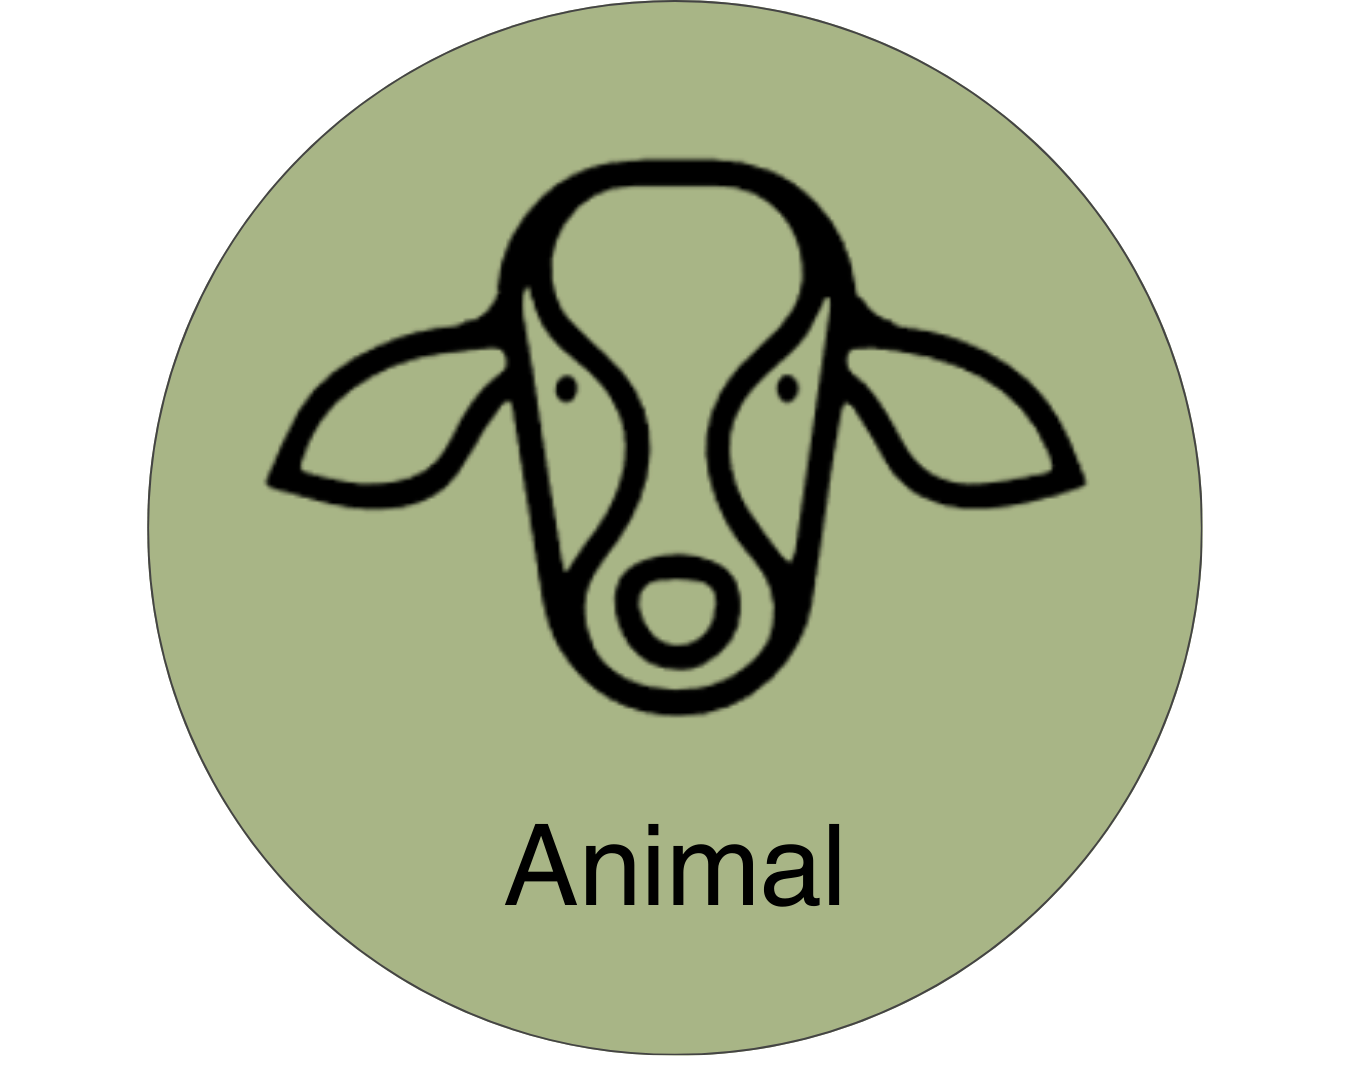
\includegraphics[width=0.4\linewidth]{resources/animal1.png}
\end{minipage}%
\hfill
\begin{minipage}[t]{0.6\textwidth}
  \vspace{0pt}

  \begin{itemize}
      \item Individual animal growth
      \item Gestation and milk production
      \item Estimation of nutrient requirements and feed intake
      \item Enteric emission and manure excretion 
  \end{itemize}
\end{minipage}
\end{figure}
\par\noindent\justifying

Animals in the RuFaS model are divided into 5 life stages and a culling stage that were established based on the different management and physiological processes that need to be simulated for each class. The 5 classes and culling stage are described in more detail later in this document, but include: calves, heifers I, heifers II, heifers III, cow, and culled. 

The attributes that define the animal characteristics and management are provided by the user and are comprehensively described in the inputs section of this module. When a simulation begins, the herd is populated by a semi-random draw of animals from a large, existing set of animal objects. This process and the process for regenerating the population of animals used to initialize the herd are described in detail in the \hyperref{herdinit}{Herd Initialization Section}. The initially selected animal objects are then grouped into pens based on their life stage and the user-provided pen information. Once the herd has been set up, a regular progression of functions is called each day to simulate and report outputs of the processes required to manage the herd and the processes that define each animal’s development and production. These daily updates are grouped into two classes in the RuFaS model: herd level daily routines (HerdManager) and animal level daily routines (AnimalManager). At the start of each day, the Herd-level daily update cycles through all the animals to call their daily update functions. Then based on the changes for each animal that resulted from the animal level daily updates, the HerdManager changes the animal life-stages, moves them to new pens, and removes them from the herd. If the herd size has decreased too much, the HerdManager will purchase new Heifer III animals to maintain the adult herd size. The HerdManager then checks if it is time to formulate a new diet (at a user-specified interval), summarizes and reports the herd statistics, and gathers and reports all of the manure excreted by the animals to pass to the Manure Module. 

Daily outputs from the Animal module are provided at a variety of scales and time steps that range from reports at the individual animal level (e.g. animal event histories), animal class level (e.g. average dry-matter intake for Heifer II’s), at the pen level (e.g. average net energy requirement or intake for Pen 3), and at the herd level (i.e. number of animals sold each day). A complete list of potential outputs from the Animal Module is provided in this document.
\vspace{1cm}


\subsection{Animal Life Cycle}
\vspace{0.2cm}

The animal life cycle is driven by Monte Carlo stochastic processes that simulate the growth, production, reproduction, and culling of individual dairy cattle animals and shares aggregated outcomes with the herd management sub-module to manage herd dynamics on a daily basis. 
 
The life cycle module represents the variation in animal performance through the use of Monte Carlo Simulation methods \parencite{reuven2017}. Monte Carlo simulation relies on random draws from probability distributions rather than assigning fixed values. In this model, two main strategies are used:
\begin{itemize}
    \item Event-based, in which a random draw from a uniform distribution (U(0,1)) is compared to the probability of an event occurring to simulate if that event occurs, and 
    \item Population-based, in which a random draw from a known distribution of attribute values is assigned to an animal at instantiation. Probability distributions used for that purpose are Normal Gaussian or Empirical. 
\end{itemize}

Each animal within the RuFaS herd progresses through five main life stages (calf, Heifer I, Heifer II, Heifer III, and Cow) as illustrated in the figure below. 
\begin{itemize}
    \item Calves progress to Heifer I when their age reaches the user-defined input for weaning day
    \item Heifer I progresses to Heifer II when their age reaches the user-defined input for breeding start day 
    \item Heifer II animals that successfully conceive become Heifer III's when the number of days left in their pregnancy is equal to the user-defined input for prefresh days (default 21)
    \item When a Heifer III calves, she becomes a Cow for the rest of her life on the RuFaS farm
    \item Cows cycle through lactating and non-lactating phases until they are removed from the herd due to a failure to conceive or a user-provided probability for sale or death within each parity (lactation).

\end{itemize}

When a HeiferIII or Cow reaches full gestation length, they start lactating and a new calf object is created. The calf is assigned a birthweight according to a user-informed random distribution. All male calves are recorded and removed from the farm on day 1 of their life. Female calves either remain on the farm or are sold on day 1, determined by an event-based Monte Carlo method informed by the user-defined percent of female calves that are kept. 



\section{Herd-level Processes and Management}
\vspace{0.5cm}

\subsection{Herd Initialization} \label{herdinit}
\vspace{0.5cm}

\begin{tcolorbox}[colback=white, colframe=black, title=Important Note]
\textit{In RuFaS code, the term “herd initialization” is used to refer to both the process of generating an animal population file and of selecting from that population to create a specific herd at the start of a simulation. In this doc, those two processes will be differentiated by calling them “Generation” and “Selection”, respectively. }
\vspace{0.2cm}

\textit{“Animal population” can refer to both groups of animals (the pool of animals generated, and the herd of animals selected). In the code, the population is sometimes referred to as “pre\_animal\_population” and “post\_animal\_population” to differentiate whether the specified group of animals exists before or after the random selection of individuals to create a herd. }
\end{tcolorbox}
\vspace{0.2cm}

\paragraph{Introduction}

Every simulation begins with a herd consisting of calves, heifers, and dry and lactating cows. This herd comes to be through a two-step process: 
\begin{enumerate}
    \item A population of animals is generated through simulation or loaded from data (pre-animal-population). The animals in that herd should reflect the attributes of animals in the herd to be modeled. 
    \item Animals are randomly selected with replacement from the pre-animal-population to be in the initial herd, based on group numbers and characteristics that reflect the distribution of animals within the herd being modeled. Note that the animals in the herd on day one will have attributes of the pre-animal-population and may deviate from the desired herd to be modeled.  
\end{enumerate}

For the rest of the simulation, animals enter the herd through birth as newborn calves or purchased replacements (heiferIII’s). 


% assumes \newcolumntype{L}[1]{>{\raggedright\arraybackslash}p{#1}}
\renewcommand{\arraystretch}{1.4}

\begin{longtable}{@{} L{5cm} L{5cm} L{5cm} @{}}
\caption{Overview of the distinct phases by which animals are created and introduced to the herd.}\\
\toprule
\multicolumn{1}{c}{\textbf{Before the simulation}} &
\multicolumn{1}{c}{\textbf{At the initiation of simulation}} &
\multicolumn{1}{c}{\textbf{During the simulation}}\\
\midrule
\endfirsthead

\multicolumn{3}{@{}l}{\textit{Table continued from previous page}}\\
\toprule
\multicolumn{1}{c}{\textbf{Before the simulation}} &
\multicolumn{1}{c}{\textbf{At the initiation of simulation}} &
\multicolumn{1}{c}{\textbf{During the simulation}}\\
\midrule
\endhead

\midrule
\multicolumn{3}{r@{}}{\textit{Continued on next page}}\\
\endfoot

\bottomrule
\endlastfoot

Generate (simulate) or load an Animal Population file (pre-animal-population).  
\vspace{0.1cm}

The animals present at the start of the simulation, and those available in the replacement market, are drawn from this file. &%

Herd is established by random selection of animals from the Animal Population to match the user-specified group sizes and age/stage distribution (post-animal-population).  
\vspace{0.1cm}

Management attributes—including lactation-curve parameters—are assigned as each animal enters the herd. &%

New animals enter via \textbf{(a)} birth or \textbf{(b)} purchase of heifers from the replacement market.  
Purchased animals inherit two attributes from the population file:
\begin{minipage}[t]{\linewidth}
\begin{itemize}
  \item Breed
  \item Mature body weight
\end{itemize}
\end{minipage}\\

\end{longtable}



\newpage
\begin{landscape}
% Suppress header/footer for all pages of the longtable
\fancypagestyle{landscapeplain}{
  \fancyhf{} % clear header and footer
  \renewcommand{\headrulewidth}{0pt}
  \renewcommand{\footrulewidth}{0pt}
}

\pagestyle{landscapeplain} % Apply to all pages in this landscape block
\textbf{Required User Inputs}
% assumes \newcolumntype{L}[1]{>{\raggedright\arraybackslash}p{#1}}
\renewcommand{\arraystretch}{1.4}

\begin{longtable}{@{} L{5cm} L{7cm} C{2cm} C{2cm} C{2cm} @{} }
\caption{User inputs in the animal input file that influence the generation of the Animal Population (pre-animal-population). The inputs of this table are found in the Herd Initialization Section}\\
\toprule
\multicolumn{1}{c}{\textbf{Variable}} &
\multicolumn{1}{c}{\textbf{Definition}} &
\multicolumn{1}{c}{\textbf{Default}} &
\multicolumn{1}{c}{\textbf{Min}} &
\multicolumn{1}{c}{\textbf{Max}}\\
\midrule
\endfirsthead

\multicolumn{3}{@{}l}{\textit{Table continued from previous page}}\\
\toprule
\multicolumn{1}{c}{\textbf{Variable}} &
\multicolumn{1}{c}{\textbf{Definition}} &
\multicolumn{1}{c}{\textbf{Default}} &
\multicolumn{1}{c}{\textbf{Min}} &
\multicolumn{1}{c}{\textbf{Max}}\\
\midrule
\endhead

\midrule
\multicolumn{3}{r@{}}{\textit{Continued on next page}}\\
\endfoot

\bottomrule
\endlastfoot

Initial\_animal\_num & The initial number of animals that serve as a starting point for the population generation simulation & 10000 & 0 & -  \\
Simulation\_days & The number of days to simulate for the population generation simulation & 5000 & 0 & -   \\

\end{longtable}
\vspace{-0.75cm}

\renewcommand{\arraystretch}{1.4}

\begin{longtable}{@{} L{5cm} L{7cm} C{2cm} C{2cm} C{2cm} @{} }
\caption{User inputs in the animal input file that influence the generation of the Animal Population (pre-animal-population). The inputs of this table are found in the Herd Initialization Section.}\\
\toprule
\multicolumn{1}{c}{\textbf{Variable}} &
\multicolumn{1}{c}{\textbf{Definition}} &
\multicolumn{1}{c}{\textbf{Default}} &
\multicolumn{1}{c}{\textbf{Min}} &
\multicolumn{1}{c}{\textbf{Max}}\\
\midrule
\endfirsthead

\multicolumn{5}{@{}l}{\textit{Table continued from previous page}}\\
\toprule
\textbf{Variable} & \textbf{Definition} & \textbf{Default} & \textbf{Min} & \textbf{Max} \\
\midrule
\endhead

\midrule
\multicolumn{5}{r@{}}{\textit{Continued on next page}}\\
\endfoot

\bottomrule
\endlastfoot

Calf\_num & Number of Calves (head) -- The initial number of pre-weaned calves & 8 & 2 & -- \\
HeiferI\_num & Number of HeiferI animals (head) -- The initial number of heifers that are weaned but not yet bred & 44 & 2 & -- \\
HeiferII\_num & Number of HeiferII animals (head) -- The initial number of heifers that are either eligible for breeding (based on user-inputted Breeding Start Day for heifers), or in early pregnancy & 38 & 2 & -- \\
HeiferIII\_num\_springers & Number of HeiferIII animals (head) -- The initial number of close-up heifers (within the user-defined close-up period, e.g., Prefresh Day) & 5 & 2 & -- \\
Cow\_num & Number of Cows (head) -- The initial number of dry and lactating cows & 100 & 6 & -- \\
Replace\_num & Replacements (head) -- Number of replacement animals available in the replacement market & 5000 & 50 & -- \\
Lactating\_fraction & Fraction of cows that are lactating. Used during herd initialization & 0.8356 & 0 & 1 \\
Parity\_fractions: 1, 2, 3, 4, 5 & Fractions of the milking animal population that are parity 1, 2, 3, 4, and 5+. The sum must equal 1.0 & 0.36, 0.26, 0.18, 0.11, 0.09 & 0 & 1 \\

\end{longtable}



\end{landscape}


\textbf{Relevant Outputs}

After the animals have been selected from the animal population to create the initial herd, a summary of the Population (pre-selection pool, aka pre-animal-population) and of the Initial herd (selected animals, aka post-animal-population) is provided to the output manager. 
\vspace{0.2cm}

Class and function: AnimalModuleReporter.report\_animal\_population\_statistics
Output variables: 
\begin{itemize}
    \item .population\_{...}
    \item .initial\_{...}
\end{itemize}

{...} includes: breed, number of animals of each class (calf, heiferI, heiferII, heiferIII, cow), number of cows by parity and lactation status, average age of animals within each class, distribution of age of animals within each class, average body weight of animals within each class, average cow days in milk, days in preg, parity, and calving interval. 




\paragraph{Methodology}

When a simulation begins, the HerdFactory class generates or loads the pre-animal-population, from which it selects and compiles the post-animal-population with an appropriate distribution of animal ages and stages to serve as the starting herd for simulation. 
\vspace{0.3cm}

\textbf{\textit{Designation of an Animal Population}}
\vspace{0.3cm}

\textbf{Option 1:} Creating a new Animal Population
An animal population can be generated as a stand-alone simulation task that creates and saves a pre-animal-population file  as the output based on the user Animal Module inputs. Or, the animal population can be generated as the first step of a regular simulation task which then uses that generated pre-animal-population to select from and create the post-animal-population to use for the subsequent herd simulation. See the documentation about Task Manager for more information about how to generate a new pre-animal-population. 
\vspace{0.2cm}

The \_generate\_animals() method creates the pre\_animal\_population, with the option to save those animals to file at the end of the generation process. 
\vspace{0.2cm}

Calves are created according to the number specified by the user (initial\_animal\_num), some are sold based on user inputs, and those remaining proceed through select daily updates (growth, reproduction, milk, and transition through the appropriate life stages) for the user-specified number of days (simulation\_days). The simulation occurs similarly to the regular life cycle simulation process, but with an extended period and large number of animals. There are a few notable distinctions:  
\begin{itemize}
    \item After 3000 days of simulation (specified in animal\_constants), a copy of each heiferIII is saved to the replacement herd. The copy is made on the day when she is ready to transition to a lactating cow (ready to give birth), so that when the copy enters the herd as a purchased heiferIII during the actual simulation, she will give birth the very next day. 
    \item If a cow has made it to parity six without being culled, she is removed from the herd. (The maximum parity of cows kept in the generated herd is five). 

\end{itemize}

After the simulation\_days number of days, the full herd contains a mixture of calves, heifers, cows, and replacements. The core status information and life history of each animal are either saved to file or passed for random sampling to create the post-animal-population. 
\vspace{0.2cm}

\textbf{Option 2:} Point to an existing Animal Population
Alternatively, the pre-animal-population will be loaded from a specified Animal Population input file consisting of calf, heifer, cow, and replacement objects. 
\vspace{0.2cm}

\textit{Herd Selection}
The \_random\_sample\_with\_replacement() method selects animals from each of the following groups: calf, heiferI, heiferII, heiferIII, replacement, lactating cows by parity for parities 1-5, and dry cows by parity for parities 1-5. Animals are sampled randomly with replacement from the pre-animal-population according to the numbers, parity fractions, and milking cow fraction specified in the animal input file. The resulting list of animals is returned as the post-animal-population and summaries of the pre- and post-animal-populations are reported to the output manager.



\subsection{Pens and Animal Grouping}

 
    \paragraph{Introduction} All animals in RuFaS are assigned to a pen which is used to summarize nutrient requirements for diet formulation and feeding, aggregate enteric methane and manure excretions for reporting and passage to the Manure Module. Each pen tracks and updates daily a list of animals in the pen, the stocking density, the average nutrient requirement of the animals in the pen, the ration being fed to that pen, the manure excreted, and the methane emitted. In addition, constant attributes of each pen include the type of pen it is (freestall, tiestall, open lot, compost bedded pack barn), the type of animals that can be in that pen, the number stalls, the manure management practices associated with that pen, and the distance to the milking parlor for lactating cows.  Each day after the HerdManager has updated the status of each animal and determined which animals need to be bought or sold, the animals are added and removed from pens as needed. 

\newpage
\begin{landscape}
% Suppress header/footer for all pages of the longtable
\fancypagestyle{landscapeplain}{
  \fancyhf{} % clear header and footer
  \renewcommand{\headrulewidth}{0pt}
  \renewcommand{\footrulewidth}{0pt}
}

\pagestyle{landscapeplain} % Apply to all pages in this landscape block

% Begin longtable
\textbf{Required User Inputs} 
\begin{center}
    \captionof{table}{The user must define at least 3 pens and for each pen, key inputs are:} 
\end{center}
\renewcommand{\arraystretch}{1.4} % More vertical space between rows
\begin{longtable}{@{} L{5cm} L{7cm} C{2cm} C{2cm} C{2cm} @{} }

\toprule
\multicolumn{1}{c}{\textbf{Variable}} & 
\multicolumn{1}{c}{\textbf{Definition}} &
\multicolumn{1}{c}{\textbf{Default}} &
\multicolumn{1}{c}{\textbf{Min}} &
\multicolumn{1}{c}{\textbf{Max}} \\
\midrule
\endfirsthead

\multicolumn{5}{@{}l}{\textit{Table continued from previous page}} \\
\toprule
\multicolumn{1}{c}{\textbf{Variable}} & 
\multicolumn{1}{c}{\textbf{Definition}} &
\multicolumn{1}{c}{\textbf{Default}} &
\multicolumn{1}{c}{\textbf{Min}} &
\multicolumn{1}{c}{\textbf{Max}} \\
\midrule
\endhead

\midrule
\multicolumn{5}{@{}r@{}}{\textit{Continued on next page}} \\
\endfoot

\bottomrule
\endlastfoot


id  & The index of the pen  & NA  & 0 & NA \\

pen\_name  & The name or identifier of a given pen  & NA  &  &  \\

animal\_combination  & The valid combinations of animal types that can be in a pen. CALF = Calves; GROWING = HeiferI's and HeiferII's; CLOSE\_UP = HeiferIII's and Dry Cows; LAC\_COWS = Lactating Cows  &    &  \multicolumn{2}{C{6cm}}{CALF, GROWING CLOSE\_UP, LAC\_COW} \\

vertical\_dist\_to\_milking\_parlor  & The elevation gain (in meters) between the pen and the milking parlor  & 0.1  &  0 & NA \\

horizontal\_dist\_to\_milking\_parlor  & The distance (in meters) between the pen and the milking parlor & 10  &  0 & NA \\

number\_of\_stalls  &  The number of stalls in the pen & 1000  &  0 & NA \\

pen\_type  &  The type of pen (freestall, tiestall, open lot, compost bedded pack barn) & freestall  & \multicolumn{2}{C{6cm}}{freestall, tiestall, open lot, compost bedded pack barn} \\

max\_stocking\_density  &  The maximum ratio of the number of animals in the pen to the number of stalls in the pen & 1.2  &  0.5 & 5 \\

manure\_management\_scenario\_id &  The ID number of the manure management practices that are used for this pen (scenarios are defined in manure management schema) & 0  &  0 & NA \\

\end{longtable}
\end{landscape}


    \textbf{Relevant Outputs}
    \begin{itemize}
        \item \textbf{number\_of\_animals\_in\_pen\_[id]\_[AnimalCombination]} reports the number of animals in each pen each day.

        \item \textbf{ration\_per\_animals\_for\_pen\_[id]\_[AnimalCombination]} - reports average dry matter intake of an animal in the pen at the time of the ration formulation.

        \item \textbf{ration\_per\_animals\_for\_pen\_[id]\_[AnimalCombination].[RUFAS\_feed\_id]} - reports the amount of each feed that is delivered per animal in the pen

        \item \textbf{ration\_nutrient\_amount\_for\_pen\_\_[AnimalCombination].[nutrient]} - is reporting the amount of each of the following nutrients that is provided by the ration per animal in the pen (all reported in kilograms unless otherwise indicated):
    \end{itemize}
    
    
\paragraph{Methodology}

\textbf{\textit{Animal Grouping}} To translate from the AnimalTypes needed to track an animal’s life stages and the combinations of animals that are allowed to be grouped into a single pen, a new variable called AnimalCombination is created that combines some AnimalTypes to facilitate sorting into pens. The AnimalCombination class is defined in enums.py and includes the following mapping from AnimalTypes to AnimalCombinations:

\begin{table}[h!]
\centering
\renewcommand{\arraystretch}{1.3}
\caption{A summary of animal types}
\begin{tabular}{@{} L{4.5cm} L{3.5cm}  @{}}
\toprule

\multicolumn{1}{c}{\textbf{Animal Combination}} &
\multicolumn{1}{c}{\textbf{Animal Types}} \\
\midrule
CALF  & Calves  \\
GROWING  & Heifer I and Heifer II  \\
CLOSE\_UP  & Heifer III and Cows (non-lactating)  \\
LAC\_COW  & Cows (lactating)  \\
\bottomrule
\end{tabular}
\end{table}  

 
 Currently there are only two options for assigning AnimalCombinations to pens. 
\vspace{0.2cm}
\begin{itemize}
    \item \textit{Option 1} - The first and most commonly used option for grouping animals is to assign one AnimalCombination to each pen such that there is at least one pen for the 4 AnimalCombinations: CALF, GROWING, CLOSE\_UP, and LAC\_COW. 
    \item \textit{Option 2} - In some cases, and especially in very small farms, a user might wish to represent a scenario where all growing animals, pregnant heifers, and non-lactating cows are housed together. In this case, there is an option to have a pen that houses both GROWING and CLOSE\_UP animals such that the there is at least one pen with each of the 3 AnimalCombination inputs: CALF, GROWING\_AND\_CLOSE\_UP, and LAC\_COW. 
\end{itemize}


    \textbf{\textit{Pen Sizing}} Due to oscillations in the exact number of animals in each animal type, it is strongly recommended that the stocking density is at least 120\% of the expected number of animals in each pen. 
    \vspace{0.2cm}
    
    \textbf{\textit{Class}} 
    \vspace{0.2cm}
    
    \textbf{Pen}
    Pens are initiated from the Pen class by the HerdManager at the beginning of the simulation and, if needed, an additional pen is created to accommodate animals if the animal numbers have exceeded the max stocking density. 

    \textbf{\textit{Noteworthy Functions}} 
    \vspace{0.2cm}
    
    \paragraph{Remove\_animals\_by\_ids} This function is called when the HerdManager calls for: remove\_animal\_from\_pen\_and\_id\_map. It is pen specific and removes the animal from the pen and the animal ID from the animal ID map that tracks the animals in the pen. 


    \paragraph{\_add\_new\_animals}This function is called by Pen.update\_animals which is in turn called by HerdManager.\_add\_animal\_to\_pen\_and\_id\_map. Thus, when HerdManager initiates addition of animals to each pen, this function executes the addition of those animals. 

    \paragraph{Set\_animal\_nutritional\_requirements}


\subsection{Ration Formulation}
The diet recipes in RuFaS are either formulated through least-cost formulation \parencite{Li2022} or provided by the user for each of 4 animal categories (calves, growing heifers, dry and close-up cows, and lactating cows). The composition of the available feeds are provided by a feed library that was adapted from the \cite{nrc2021}. The amount of feed required by the farm is tracked by pen and multiple pens of each animal category can be simulated; however, at this time, the RuFaS model can only accept 1 user-defined diet per animal category even if there are multiple simulated pens for that animal category.  

In practice, animal feeding on dairy farms is a constantly evolving process that responds to fluctuations in feed availability, animal requirements and responses, and management goals. Although the feed delivery algorithms will make small modifications to the diet recipe in response to animal nutrient requirements and adjust the total amount of feed delivered based on the number of animals and their requirements, the diversity and degree of fluctuation in the diets is less than what is expected on a commercial dairy. The RuFaS feed library can also be modified or expanded on by changing the compositions of the existing feeds or by adding new feeds. 

Regardless of whether or not a user chooses to provide their own ration or have RuFaS build and feed a ration optimized for least-cost, RuFaS needs a set of ingredients to work from. The RuFaS feed library should be consulted for the full list of ingredients and ingredients that are in both the NASEM and NRC libraries can be used. Users interested in feeding a ration that they define, need to provide a list of ingredients and their relative \% dry matter intake for each animal class (pre-weaned calves, growing heifers, close-up animals, and lactating cows). 

\vspace{0.2cm}

If a user would like RuFaS to use the list of ingredients to formulate a least-cost ration, it is imperative that proper costs are inputted for each ingredient listed, but the \% dry matter intake in the user defined ration percentages does not need to be included. Feed costs need to be entered in \$ / kg DM. RuFaS will then use all the ingredients available (based on costs and inventory available if the feed is homegrown) to create a ration that meets the nutritional requirements of the animal class and is cost-optimized. 


\begin{tcolorbox}[colback=white, colframe=black, title=Important Note]
For the time being, only one set of feeds and ration formula can be provided for each animal class. 
\end{tcolorbox}







\subsubsection{Energy and Nutrition Requirements}

\paragraph{NRC: Calculating Nutrient Requirements of Dairy Cattle} 

Below are the calculations utilized based on the energy and nutrient requirements of dairy cattle as reported by the NRC and more recently the NASEM \parencite{nrc2001, nrc2021}.
\vspace{0.2cm}

Calculations are included for the following requirement categories:
\begin{itemize}
    \item Energy (Maintenance, Activity, Growth, Pregnancy, Lactation)
    \item Protein (Maintenance, Growth, Pregnancy, Lactation)
    \item Minerals (Maintenance, Growth, Pregnancy, Lactation)
    \item Dry Matter Intake
    \item Amino Acids (NASEM only) 
\end{itemize}
\vspace{0.2cm}

Where appropriate, requirement calculations are differentiated by animal age and reproductive status.
\vspace{0.5cm}

\subsubsection{Nutrient Requirements of Dairy Cattle (NRC)} 

    \textbf{ Energy Requirements} For details about the variables included in each calculation, please refer to the energy requirements key.
    \vspace{0.2cm}
    
    \begin{itemize}
        \item \textbf{\textit{Maintenance}} - The maintenance requirement is calculated based on metabolic body weight (body weight\(^ {0.75}\)).
        
        \vspace{0.2cm}
        \underline {Lactating and Dry Cows}
        
        \vspace{0.25cm}
\begin{center}
    \(CBW = MW * 0.06275\)
\end{center}
\vspace{0.5cm}
            {\raggedleft \textbf{[AN.NRC.1]}\par}

\vspace{0.25cm}
\begin{center}
    \(CW = {(18 + (DOP - 190) * 0.665) * ( \frac{CBW}{45}), if DOP > 190.0}\)
\end{center}
\vspace{0.5cm}
            {\raggedleft \textbf{[AN.NRC.2]}\par}
\textit{\small Otherwise}
\vspace{0.25cm}

\begin{center}
    \(NEmaint = 0.08 * (BW - CW)^{0.75}\)
\end{center}
\vspace{0.5cm}
            {\raggedleft \textbf{[AN.NRC.3]}\par}

        \vspace{0.2cm}
        \underline {Heifers} -The maintenance requirement is calculated based on metabolic body weight (body weight\(^{0.75}\)), body condition score, and the previous month's temperature.
        \vspace{0.25cm}

    
\begin{center}
    \(CBW = MW * 0.06275\)
\end{center}
\vspace{0.5cm}
            {\raggedleft \textbf{[AN.NRC.1]}\par}

\vspace{0.25cm}
\begin{center}
    \(CW = {(18 + (DOP - 190) * 0.665) * ( \frac{CBW}{45}), if DOP > 190.0}\)
\end{center}
\vspace{0.5cm}
            {\raggedleft \textbf{[AN.NRC.2]}\par}
\textit{\small Otherwise}
\vspace{0.25cm}


\begin{center}
    \(BCS9 = (BCS5 - 1) * 2 + 1\)
\end{center}
\vspace{0.5cm}
            {\raggedleft \textbf{[AN.NRC.6]}\par}

\vspace{0.25cm}
\begin{center}
    \(NEmaint = (BW - CW)^{0.75} * (0.086 * (0.8 + (BCS9 - 5) * 0.05) + 0.0007 * (20 - PrevTemp))\)
\end{center}
\vspace{0.5cm}
            {\raggedleft \textbf{[AN.NRC.7]}\par}

\vspace{0.25cm}

        \item \textbf{\textit {Activity}} - Activity requirement is proportional to body weight and daily walking distance. A grazing system and hilly topography will cost additional energy. 

        \vspace{0.2cm}
        \underline {Lactating and Dry Cows}
        \vspace{0.25cm}

    
\begin{center}
    \(NEa1 = 0.0012 * BW\) if Housing = Grazing 0
\end{center}
\vspace{0.5cm}
            {\raggedleft \textbf{[AN.NRC.8]}\par}
\textit{\small Otherwise}
\vspace{0.25cm}

\begin{center}
    \(NEa2 = 0.006 * BW\) if Topography = Hilly 0
\end{center}
\vspace{0.5cm}
            {\raggedleft \textbf{[AN.NRC.9]}\par}
\textit{\small Otherwise}
\vspace{0.25cm}

\begin{center}
    \(NEa2 = 0.Distance * 0.00045 * BW + NEa1 + NEa2\) 
\end{center}

\vspace{0.5cm}
            {\raggedleft \textbf{[AN.NRC.10]}\par}
            
        \vspace{0.2cm}
        \underline {Heifers}
        \vspace{0.25cm}
        
\begin{center}
    \(NEa1 = 0.0009 * BW + 0.0016 * BW\) if Housing = Grazing 0
\end{center}
\vspace{0.5cm}

            {\raggedleft \textbf{[AN.NRC.11]}\par}
\textit{\small Otherwise}
\vspace{0.25cm}

\begin{center}
    \(NEa2 = 0.006 * BW\) if Topography = Hilly 0
\end{center}
\vspace{0.5cm}

            {\raggedleft \textbf{[AN.NRC.12]}\par}
            \vspace{0.25cm}
            
\textit{\small Otherwise}
\vspace{0.25cm}

\begin{center}
    \(NEa2 = 0.Distance * 0.00045 * BW + NEa1 + NEa2\) 
\end{center}
\vspace{0.5cm}

            {\raggedleft \textbf{[AN.NRC.10]}\par}

\vspace{0.5cm}


        \item \textbf{\textit{Growth}}
        
        \vspace{0.2cm}
        \underline {Lactating and Dry Cows} Cows will continue to grow toward their mature body weight until the end of their second lactation. 
        \vspace{0.25cm}
        
\begin{center}
    \(MSBW = 0.96 * MW\)
\end{center}
\vspace{0.5cm}
            {\raggedleft \textbf{[AN.NRC.13]}\par}

\vspace{0.25cm}
\begin{center}
    \(SBW = 0.96 * BW\)
\end{center}

\vspace{0.5cm}
            {\raggedleft \textbf{[AN.NRC.14]}\par}
\vspace{0.25cm}

\begin{center}
    \(EBW = 0.96 * SBW\)
\end{center}
\vspace{0.5cm}

            {\raggedleft \textbf{[AN.NRC.15]}\par}
\vspace{0.25cm}

\begin{center}
    \(EQSBW = (SBW - CW) *\frac{478}{MSBW} SBW\)
\end{center}
\vspace{0.5cm}

            {\raggedleft \textbf{[AN.NRC.16]}\par}
\vspace{0.25cm}

\begin{center}
    \(ADG = \frac{(0.92 - 0.82) * MSBW}{CI}, if Parity = 1 \frac{(1 - 0.92) * MSBW}{CI}, if Parity = 2.0, if Parity > 2\)
\end{center}
\vspace{0.5cm}

            {\raggedleft \textbf{[AN.NRC.17]}\par}
\vspace{0.25cm}

\begin{center}
    \(EQEBG = 0.956 * ADG\)
\end{center}
\vspace{0.5cm}

            {\raggedleft \textbf{[AN.NRC.18]}\par}
    \vspace{0.25cm}
    
\begin{center}
    \(EQEBW = 0.891 * EQSBW\)
\end{center}

\vspace{0.5cm}
            {\raggedleft \textbf{[AN.NRC.19]}\par}
\vspace{0.25cm}

\begin{center}
    \(NEg = 0.0635 * EQEBW^{0.75} * EQEBG^{1.097}\)
\end{center}

\vspace{0.5cm}
            {\raggedleft \textbf{[AN.NRC.20]}\par}
            
        \vspace{0.2cm}
        \underline {Heifers}
\vspace{0.25cm}

\begin{center}
    \(ADG = \frac{0.55 * MSBW - SBW}{(Age1stBred - Age) * 30.4},\ before\ breeding\ \frac{0.82 * MSBW - SBW}{(Age1st - Age) * 30.4},\ after\ breeding\)
\end{center}

\vspace{0.5cm}
            {\raggedleft \textbf{[AN.NRC.21]}\par}
\vspace{0.2cm}

\begin{center}
    \(EQEBG = 0.956 * ADG\)
\end{center}

\vspace{0.5cm}
            {\raggedleft \textbf{[AN.NRC.22]}\par}
\vspace{0.2cm}

\begin{center}
    \(EQEBW = 0.891 * EQSBW\)
\end{center}

\vspace{0.5cm}
            {\raggedleft \textbf{[AN.NRC.23]}\par}
\vspace{0.2cm}

\begin{center}
    \(NEg = 0.0635 * EQEBW^{0.75} * EQEBG^{1.097}\)
\end{center}

\vspace{0.5cm}
            {\raggedleft \textbf{[AN.NRC.24]}\par}

\vspace{0.5cm}



        \item \textbf{\textit{Pregnancy}}
\vspace{0.2cm}

\begin{center}
    \(MEpreg = (2 * 0.00159 * DOP - 0.0352) * \frac{CBW}{45} * 0.14, if DOP > 190.0\)
\end{center}

\textit{\small Otherwise}

\vspace{0.5cm}
            {\raggedleft \textbf{[AN.NRC.25]}\par}
\vspace{0.2cm}

\begin{center}
    \(NEpreg = MEpreg * 0.664\)
\end{center}

\vspace{0.5cm}
            {\raggedleft \textbf{[AN.NRC.26]}\par}

\vspace{0.5cm}



        \item \textbf{\textit{Lactation}}
\vspace{0.2cm}

\begin{center}
    \(Milk_{\text{Energy}} = 0.0929 * Fat\_Milk + \frac{0.0563}{0.93} * TP\_Milk + 0.0395 * Lactose\_Milk\)
\end{center}

\vspace{0.5cm}
            {\raggedleft \textbf{[AN.NRC.27]}\par}

\vspace{0.2cm}

\begin{center}
    \(NElact = Milken * Milk\)
\end{center}

\vspace{0.5cm}
            {\raggedleft \textbf{[AN.NRC.28]}\par}
            
\vspace{0.5cm}


    \end{itemize}

    
    \textbf{ Protein Requirements} Reporting of protein requirements is divided into 4 components: maintenance, growth, pregnancy, and lactation (all in metabolizable protein). For details about the variables included in each calculation, please refer to the protein requirements key.
    \vspace{0.2cm}

    \begin{itemize}
                \item \textbf{\textit{Total Protein}}
\vspace{0.2cm}

\begin{center}
    \(MPreq = MPm + MPg + MPpreg + MPlact\)
\end{center}

\vspace{0.5cm}
            {\raggedleft \textbf{[AN.NRC.36]}\par}
        
                \item \textbf{\textit{Maintenance}}
        
        \vspace{0.2cm}
        \underline {Lactating and Dry Cows}
        \vspace{0.2cm}

\begin{center}
    \(MPm = 0.3 * (BW - CW)^{0.6} + 4.1 * (BW - CW)^{0.5} + (DMI * 1000 * 0.03 - 0.5 * (\frac{MPbact}{0.8} - MPbact)) + 0.4 * 11.8 * \frac{DMI}{0.67}\)
\end{center}

\vspace{0.5cm}
            {\raggedleft \textbf{[AN.NRC.29]}\par}
        
                \item \textbf{\textit{Growth}}
        \vspace{0.2cm}


        \underline {Lactating and Dry Cows}
        \vspace{0.2cm}

\begin{center}
    \(NPg = 0, if ADG = 0, ADG * (268 - 29.4 * \frac{NEg}{ADG})\)
\end{center}

\vspace{0.5cm}
            {\raggedleft \textbf{[AN.NRC.30]}\par}
        \vspace{0.2cm}

\begin{center}
    \(EffMP\_NPg = \frac{(83.4 - 0.114 * EQSBW)}{100}, if EQSBW \leq 478, 0
    .28908\)
\end{center}
\vspace{0.5cm}

            {\raggedleft \textbf{[AN.NRC.31]}\par}
\textit{\small Otherwise}
        \vspace{0.2cm}

\begin{center}
    \(MPg = \frac{NPg}{EffMP\_NPg}\)
\end{center}
\vspace{0.5cm}

            {\raggedleft \textbf{[AN.NRC.32]}\par}

            
        
        \underline {Heifers}
        \vspace{0.2cm}

\begin{center}
    \(Npg = 0, if ADG = 0 ADG * (268 - 29.4 * \frac{NEg}{ADG})\)
\end{center}

\vspace{0.5cm}
            {\raggedleft \textbf{[AN.NRC.33]}\par}
        \vspace{0.2cm}

\begin{center}
    \(EffMP\_NPg = \frac{(83.4 - 0.114 * EQSBW)}{100}, if EQSBW \leq 478, 0
    .28908\)
\end{center}
\vspace{0.5cm}

            {\raggedleft \textbf{[AN.NRC.34]}\par}
\textit{\small Otherwise}
        \vspace{0.2cm}

\begin{center}
    \(MPg = \frac{NPg}{EffMP\_NPg}\)
\end{center}
\vspace{0.5cm}

            {\raggedleft \textbf{[AN.NRC.35]}\par}
\vspace{0.2cm}

\begin{center}
    \(MPreq = MPm + MPg + MPpreg + MPlact\)
\end{center}

\vspace{0.5cm}
            {\raggedleft \textbf{[AN.NRC.36]}\par}
            
\vspace{0.5cm}
                \item \textbf{\textit{Pregnancy}}
\vspace{0.2cm}

\begin{center}
    \(MPpreg = (0.69 * DOP - 69.2) * \frac{CBW}{45 * 0.33}, if DOP > 190.0\)
\end{center}

\vspace{0.5cm}
            {\raggedleft \textbf{[AN.NRC.37]}\par}
\vspace{0.25cm}
            
                \item \textbf{\textit{Lactation}}
\vspace{0.2cm}

\begin{center}
    \(MPlact = Milk * \frac{TP_{\text{Milk}}}{100} * \frac{1000}{0.67}\)
\end{center}

\vspace{0.5cm}
            {\raggedleft \textbf{[AN.NRC.38]}\par}
\vspace{0.5cm}

    \end{itemize}


\renewcommand{\arraystretch}{1.3}
\begin{longtable}{@{} L{3.5cm} L{3.5cm} L{2.5cm} @{}}
\caption{Key variables used in protein requirement calculations.} \\
\toprule
\textbf{Variable} & \textbf{Description} & \textbf{Units} \\
\midrule
\endfirsthead

\toprule
\textbf{Variable} & \textbf{Description} & \textbf{Units} \\
\midrule
\endhead

\multicolumn{3}{r}{\textit{Continued on next page}} \\
\endfoot

\bottomrule
\endlastfoot
    
EffMP\_NPg & Efficiency of converting metabolizable protein or net protein  &  \\
MPg & Metabolizable protein requirement for growth  & g\\
MPlact & Metabolizable protein requirement for lactation  & g \\
MPpreg &  Metabolizable protein requirement for pregnancy & g \\
NPg & Net protein requirement for growth  & g \\

    \end{longtable}



    \textbf{ Mineral Requirements} 
    \begin{tcolorbox}[colback=white, colframe=black, title=Important Note]
        Only calcium (Ca) and phosphorus (P) requirements are considered currently. For details about the variables included in each calculation, please refer to the mineral requirements key.
    \end{tcolorbox}

    \begin{itemize}
        \item \textbf{\textit{Maintenance}} 
        \vspace{0.2cm}
        
        \underline{Lactating and Dry Cows}
\vspace{0.2cm}

Calcium Equations
\begin{center}
    \(Ca_{\text{main}} = 0.031 * BW + 0.08 * \frac{BW}{100},\) for lactating cows\\
    \vspace{0.2cm}
    \(Ca_{\text{main}} = 0.0.0154 * BW + 0.08 * \frac{BW}{100},\) for dry cows
\end{center}

\vspace{0.5cm}
            {\raggedleft \textbf{[AN.NRC.39]}\par}

\vspace{0.5cm}
Phosphorus Equations
\vspace{0.5cm}

\begin{center}
    \(P_{\text{main}} = 1 * DMI + 0.002 * BW, \) for lactating cows\\
    \vspace{0.25cm}
    \(P_{\text{main}} = 0.8 * DMI + 0.002 * BW, \) for dry cows
\end{center}

\vspace{0.5cm}
            {\raggedleft \textbf{[AN.NRC.40]}\par}
\vspace{0.25cm}

        {\underline{Heifers}}
                \vspace{0.2cm}

Calcium Equation
\begin{center}
    \(Ca_{\text{main}} = 0.0.0154 * BW + 0.08 * \frac{BW}{100}, \)
\end{center}

\vspace{0.5cm}
            {\raggedleft \textbf{[AN.NRC.41]}\par}
            \vspace{0.5cm}

Phosphorus Equation
\begin{center}
    \(P_{\text{main}} =  0.8 * DMI + 0.002 * BW, \)
\end{center}

\vspace{0.5cm}
            {\raggedleft \textbf{[AN.NRC.42]}\par}
\vspace{0.5cm}

        \item \textbf{\textit{Growth}} 
\vspace{0.2cm}

Calcium Equation
\begin{center}
    \(Ca_{\text{growth}} = 9.83 * MW^{0.22} * BW^{-0.22} * \frac{ADG}{0.96}\)
\end{center}

\vspace{0.5cm}
            {\raggedleft \textbf{[AN.NRC.43]}\par}
            
\vspace{0.5cm}
Phosphorus Equation
\vspace{0.2cm}
                
\begin{center}
    \(P_{\text{growth}} = (1.2 + 4.635 * MW^{0.22} * BW^{-0.22}) * \frac{ADG}{0.96} \) 
\end{center}
\vspace{0.5cm}
            {\raggedleft \textbf{[AN.NRC.44]}\par}
\vspace{0.5cm}

            
        \item \textbf{\textit{Pregnancy}}  
\vspace{0.2cm}

Calcium Equation

\begin{center}
    \(Ca_{\text{preg}} = 0.02456 * exp0.05581 - 0.00007 * DOP * DOP - 0.02456 * exp0.05581 - 0.00007 * - 1 * DOP - 1, if DOP > 190.0, else\)
\end{center}

\vspace{0.5cm}
            {\raggedleft \textbf{[AN.NRC.45]}\par}
\vspace{0.5cm}

Phosphorus Equation
                
\begin{center}
    \(P_{\text{preg}} = 0.02743 * exp 0.05527 - 0.000075 * DOP * DOP - 0.02743 * exp0.05527 - 0.000075 * DOP - 1 * (DOP - 1),\) \\
    \vspace{0.2cm}
    
    \textbf{If:} \( DOP > 190.0\ else\)
\end{center}

\vspace{0.5cm}
            {\raggedleft \textbf{[AN.NRC.46]}\par}
\vspace{0.5cm}

        \item \textbf{\textit{Lactation}} 
        \vspace{0.2cm}

Calcium Equation
\begin{center}
    \(Ca_{\text{lact}} = 1.22 * Milk\)
\end{center}

\vspace{0.5cm}
            {\raggedleft \textbf{[AN.NRC.47]}\par}
\vspace{0.5cm}

Phosphorus Equation
                
\begin{center}
    \(P_{\text{lact}} = 0.9 * Milk \)
\end{center}

\vspace{0.5cm}
            {\raggedleft \textbf{[AN.NRC.48]}\par}
\vspace{0.5cm}

        \item \textbf{\textit{Total Minerals}}  
                \vspace{0.2cm}

Calcium Equation
\begin{center}
    \(Ca_{\text{req}} = Ca_{\text{main}} + Ca_{\text{growth}} + Ca_{\text{preg}} + Ca_{\text{lact}}\)
\end{center}

\vspace{0.5cm}
            {\raggedleft \textbf{[AN.NRC.49]}\par}
\vspace{0.5cm}

Phosphorus Equation
\begin{center}
    \(P_{\text{req}} = P_{\text{main}} + P_{\text{growth}} + P_{\text{preg}} + P_{\text{lact}}\)
\end{center}

\vspace{0.5cm}
            {\raggedleft \textbf{[AN.NRC.50]}\par}
\vspace{0.5cm}

    \end{itemize}


\renewcommand{\arraystretch}{1.3}
\begin{longtable}{@{} L{3.5cm} L{3.5cm} L{2.5cm} @{}}
\caption{Key variables used in mineral requirement calculations.}  \\
\toprule
\textbf{Variable} & \textbf{Description} & \textbf{Units} \\
\midrule
\endfirsthead

\toprule
\textbf{Variable} & \textbf{Description} & \textbf{Units} \\
\midrule
\endhead

\multicolumn{3}{r}{\textit{Continued on next page}} \\
\endfoot

\bottomrule
\endlastfoot
    

Ca\(_{\textbf{main}}\) & Calcium maintenance requirement & g \\
Ca\(_{\textbf{growth}}\) & Calcium growth requirement & g \\
Ca\(_{\text{lact}}\) & Calcium lactation requirement & g \\
Ca\(_{\text{preg}}\)  & Calcium pregnancy requirement & g \\
Ca\(_{\textbf{req}}\) & Total calcium requirement  & g \\
DOP  &  Days of pregnancy & d \\
P\(_{\text{growth}}\) & Phosphorus growth requirement & g \\
P\(_{\text{lact}}\)  &  Phosphorus lactation requirement & g \\
P\(_{\text{main}}\) & Phosphorus maintenance requirement  & g \\
P\(_{\text{preg}}\)  &  Phosphorus pregnancy requirement & g \\
P\(_{\text{req}}\)  &  Total phosphorus requirement & g \\
    \end{longtable}



    \textbf{{Dry Matter Intake (DMI) Estimation}} 
    \vspace{0.1cm}
    
    Estimations are different for lactating cows and dry cows.  For details about the variables included in each calculation, please refer to the DMI requirements key.
    \vspace{0.2cm}
    
    The sum of DMI of each feed is assumed to be less than the estimated DMI:
                \vspace{0.2cm}
                
\begin{center}
    \(\sum_{i}Feed_{i} < DMIest\)
\end{center}

        \begin{itemize}
        \item \textbf{\textit{Lactating Cows}}
                \vspace{0.2cm}
                
\begin{center}
    \(FCM = (0.4 * Milk) + (15 * Fat\_Milk * \frac{Milk}{100})\)
\end{center}

\vspace{0.5cm}
            {\raggedleft \textbf{[AN.NRC.51]}\par}
\vspace{0.5cm}

\begin{center}
    \(DMIest = (0.372 * FCM + 0.0968 * BW^{0.75}) * (1 - exp - 0.192 * WOL + 3.67)\)
\end{center}

\vspace{0.5cm}
            {\raggedleft \textbf{[AN.NRC.52]}\par}
\vspace{0.5cm}

        \item \textbf{\textit{Dry Cows}}
\vspace{0.5cm}

\begin{center}
    \(DMIest = (\frac{(1.97 - 0.75 * exp(0.16 * (DOP - 280)))}{100}) * BW\)
\end{center}

\vspace{0.5cm}
            {\raggedleft \textbf{[AN.NRC.53]}\par}
\vspace{0.5cm}

        \item \textbf{\textit{Heifers}}
\vspace{0.5cm}

If the heifer is \textbf{less} than 365 days old:
\begin{center}
    \(DMIest = (BW^{0.75} * \frac{(0.2435 * NEadj - 0.0466 * NEadj^{2} - 0.0869)}{NEadj}) - PREGadj \)
\end{center}

\vspace{0.5cm}
            {\raggedleft \textbf{[AN.NRC.54]}\par}
\vspace{0.5cm}

If the heifer is \textbf{more} than 365 days old:
\begin{center}
    \(DMIest = (BW^{0.75} * \frac{(0.2435 * NEadj - 0.0466 * NEadj^{2} - 0.1128)}{NEadj}) - PREGadj \)
\end{center}

\vspace{0.5cm}
            {\raggedleft \textbf{[AN.NRC.55]}\par}
\vspace{0.5cm}

    \end{itemize}


\renewcommand{\arraystretch}{1.3}
\begin{longtable}{@{} L{2.5cm} L{3.5cm} L{4.5cm} @{}}
\caption{Key variables used in DMI requirement calculations.} \\
\toprule
\textbf{Variable} & \textbf{Description} & \textbf{Units} \\
\midrule
\endfirsthead

\toprule
\textbf{Variable} & \textbf{Description} & \textbf{Units} \\
\midrule
\endhead

\multicolumn{3}{r}{\textit{Continued on next page}} \\
\endfoot

\bottomrule
\endlastfoot

DMIest     & Dry matter intake estimation & kilogram (kg)  \\
DOP        & Days of pregnancy & days \\
NEadj      & the adjustment for the net energy (NE) concentration of the diet & if the NE concentration < 1 mcal/kg DM, then = 0.95 \newline if the concentration $>$ 1 mcal/kg DM, then is = to the NE concentration \\
PREGadj    & the adjustment for pregnancy status & if DOP $>$ 210 \newline 1 + ((210 - DOP) * 0.0025) \\
WOL        & Week of lactation & Units are the integer part of days \(\frac{DIM}{7}\) \\


    \end{longtable}






\paragraph{NASEM: Calculating Nutrient Requirements of Dairy Cattle: Eighth Revised Edition} 

    \textbf{ Energy Requirements} 
    The maintenance requirement is calculated based on metabolic body weight (MBW, body weight\(^{0.75}\)) adjusted for the tissues associated with pregnancy. For details about the variables included in each calculation, please refer to the energy requirements key.
    \vspace{0.2cm}

\begin{itemize}
    \item \textbf{\textit{Maintenance}}
    \vspace{0.2cm}
    
        \underline {Lactating and Dry Cows}
        For Lactating cows, the body weight is adjusted both for the gravid uterine tissues and the uterine tissues for normal activity in confinement conditions, otherwise include adjustments for activity requirements under grazing conditions. 
        
        \vspace{0.25cm}
\begin{center}
    \(NEmaint = 0.10 * (MBW - GrUterW - UterW)^{0.75}\)
\end{center}
\vspace{0.5cm}
            {\raggedleft \textbf{[AN.NSM.1]}\par}
\vspace{0.25cm}

\begin{center}
    \(GrUterW = (CBW * 1.825) * exp^{-(0.0243 - (0.0000245 * DOP))*(280 - DOP)} \)
\end{center}
\vspace{0.5cm}
            {\raggedleft\textbf{[AN.NSM.2]} \par}
\vspace{0.25cm}

\begin{center}
    \(UterW = ((CBW * 0.2288 - 0.204) * \exp^{-0.2 * DyLact} + 0.204)\)
\end{center}
\vspace{0.5cm}
            {\raggedleft\textbf{[AN.NSM.3]} \par}
\vspace{0.25cm}

\begin{center}
    \(CW = inputvariable, \)
\end{center}
\vspace{0.5cm}

\textit{\small Otherwise}
\vspace{0.25cm}

\begin{center}
    \(CBW = MW * 0.06275\)
\end{center}
\vspace{0.5cm}
            {\raggedleft \textbf{[AN.NSM.4]}\par}

        \vspace{0.2cm}
        \underline {Heifers}
        For heifers, the maintenance energy requirement is only adjusted for the gravid uterine weight:
        \vspace{0.25cm}

    
\begin{center}
    \(NEmain = 0.10 * (BW - GrUterW)^{0.75}\)
\end{center}
\vspace{0.5cm}
            {\raggedleft \textbf{[AN.NSM.5]}\par}
\vspace{0.25cm}

        \item \textbf{\textit {Activity}} - Activity requirement is proportional to body weight and daily walking distance. A grazing system and hilly topography will cost additional energy. 
        \vspace{0.25cm}

    
\begin{center}
    \(NEa1 = \frac{(Dt\_PastIn)}{DtDMIn}\) if $<$ 0.005, then 0
\end{center}
\vspace{0.5cm}
            {\raggedleft \textbf{[AN.NSM.6]}\par}
            \vspace{0.2cm}
            
\textit{\small Otherwise}

\begin{center}
    \(NEa1 = 0.0075 * BW^{0.75} * ( \frac{(600 - 12 * DtPastSupplIn)}{600})\) if \( \geq \) 0.005, then 0
\end{center}
\vspace{0.5cm}
            {\raggedleft \textbf{[AN.NSM.7]}\par}
            \vspace{0.2cm}

Energy requirements for walking to and from the milking parlor are estimated as follows:
        \vspace{0.25cm}

    
\begin{center}
    \(NEa2 = 0.00035 * \frac{(DistParlor)}{1000} * TripParlor * BW\) 
\end{center}
\vspace{0.5cm}
            {\raggedleft \textbf{[AN.NSM.8]}\par}
            \vspace{0.2cm}

\begin{center}
    \(NEa3 = 0.0067 * \frac{(EnvTopoParlor)}{1000} * BW\) 
\end{center}
\vspace{0.5cm}
            {\raggedleft \textbf{[AN.NSM.9]}\par}
            \vspace{0.2cm}
            
\begin{center}
    \(NEa = NEa1 + NEa2 + NEa3\) 
\end{center}
\vspace{0.5cm}

            {\raggedleft \textbf{[AN.NSM.10]}\par}
            \vspace{0.2cm}     

        \item \textbf{\textit {Growth}} In \textcite{nrc2021}, body frame gain (fat + protein) corresponds to the true growth and it is part of the calculation which is further partitioned into body reserves or condition gain (or loss), and pregnancy-associated gain (considered a pregnancy requirement). 
        \vspace{0.15cm}

        The value shown below was calculated but was never utilized in any further calculations in the model’s current version. Thus, it has been omitted from the model and remains solely as a reference to past versions of the model.
\vspace{0.5cm}

\begin{center}
    \(EBW = 0.85 * BW\) 
\end{center}
\vspace{0.5cm}

            {\raggedleft \textbf{[AN.NSM.11]}\par}
            \vspace{0.2cm} 
            
\begin{center}
    \(EBG = 0.85 * ADG\) 
\end{center}
\vspace{0.5cm}

            {\raggedleft \textbf{[AN.NSM.12]}\par}
            \vspace{0.2cm} 

\begin{center}
    \(FatADG = (0.067 + 0.375 * (\frac{BW}{MW})) * \frac{EBG}{ADG}\) 
\end{center}
\vspace{0.5cm}

            {\raggedleft \textbf{[AN.NSM.13]}\par}
            \vspace{0.2cm} 

\begin{center}
    \(ProtADG = (0.201 + 0.081 * (\frac{BW}{MW})) * \frac{EBG}{ADG}\) 
\end{center}
\vspace{0.5cm}

            {\raggedleft \textbf{[AN.NSM.14]}\par}
            \vspace{0.2cm} 
\begin{center}
    \(REFADG = 9.4 * FatADG + 5.55 * ProtADG\) 
\end{center}
\vspace{0.5cm}

            {\raggedleft \textbf{[AN.NSM.15]}\par}
            \vspace{0.2cm}

\begin{center}
    \(MEFrameADG = \frac{REFADG}{0.4}\) 
\end{center}
\vspace{0.5cm}

            {\raggedleft \textbf{[AN.NSM.16]}\par}
            \vspace{0.2cm}

\begin{center}
    \(NElFrameADG = \frac{REFADG}{0.61}\) 
\end{center}
\vspace{0.5cm}

            {\raggedleft \textbf{[AN.NSM.17]}\par}
            \vspace{0.2cm}
\vspace{0.5cm}



        \item \textbf{\textit{Pregnancy}} - Daily rates of wet tissue deposition (kg/d) are derived from equations \textbf{[AN.NSM.2]} and \textbf{[AN.NSM.3]} as defined above.
\vspace{0.2cm}

\textit{\small During Gestation}
\vspace{0.2cm}

\begin{center}
    \(GrUterWGain = (0.0243 - (0.0000245 * DayGest)) * GrUterW\)
\end{center}
\vspace{0.5cm}

            {\raggedleft \textbf{[AN.NSM.18]}\par}
\vspace{0.2cm}

\textit{\small During Involution}
\vspace{0.2cm}

\begin{center}
    \(MEpreg = (2 * 0.00159 * DOP - 0.0352) * \frac{CBW}{45} * 0.14, if DOP > 190.0\)
\end{center}
\vspace{0.5cm}

            {\raggedleft \textbf{[AN.NSM.19]}\par}
\vspace{0.2cm}

\textbf{Otherwise}
\vspace{0.25cm}

\begin{center}
    \(NEpreg = MEpreg * 0.64\)
\end{center}
\vspace{0.5cm}

            {\raggedleft \textbf{[AN.NSM.20]}\par}
\vspace{0.2cm}

        \item \textbf{\textit{Lactation}}
\vspace{0.2cm}

\begin{center}
    \(MilkEn = (0.0929 * Fat\_Milk + 0.0547 * Prot\_Milk + 0.0395 * Lact\_Milk)\)
\end{center}

\vspace{0.5cm}
            {\raggedleft \textbf{[AN.NSM.21]}\par}

\vspace{0.2cm}

If true protein, (TP\_Milk) is measured, its energy content is adjusted to account for the energy of Non-Protein-Nitrogen (NPN), then use the following equation. 
\vspace{0.2cm}

\begin{center}
    \(MilkEn = (0.0929 * Fat\_Milk + 0.0585 * TP\_Milk + 0.0395 * Lact\_Milk)\)
\end{center}

\vspace{0.5cm}
            {\raggedleft \textbf{[AN.NSM.22]}\par}

\vspace{0.5cm}


\end{itemize}

    \textbf{ Protein Requirements} are divided into 4 components: maintenance, growth, pregnancy, and lactation (all in MP). The last is defined as the sum of rumen undegraded protein (RUP + microbial protein (MICP)). Requirements for EEA are also included in \textcite{nrc2021} but have not yet been implemented.
    \vspace{0.2cm}
    
    Each physiological function is quantified in terms of TP (true protein), instead of CP (crude protein).
    \vspace{0.2cm}
    
    To convert both net protein and net amino acid values to a metabolizable basis, net values have to be divided into the calculated efficiencies for each physiological function. Efficiencies can be either fixed or combined for lactating cows. For simplicity, requirements were included on a fixed basis. For details about the variables included in each calculation, please refer to the protein requirements key.
    \vspace{0.5cm}

\begin{itemize}
    \item \textbf{\textit{Maintenance}} - The protein requirements for non-productive functions (the quantification of protein secretion and accretion), include: scurf + endogenous urinary loss + metabolic fecal protein.
    \begin{enumerate}
        \item \underline {Scurf Protein}
        \vspace{0.2cm}

\begin{center}
    \(NPscurf = 0.20 * BW^{0.60} * 0.85\)
\end{center}

\vspace{0.5cm}
            {\raggedleft \textbf{[AN.NSM.23]}\par}
        \vspace{0.2cm}

\begin{center}
    \(NetAAscurf = NPscurf * \frac{AACorrScurf}{100}\)
\end{center}

\vspace{0.5cm}
            {\raggedleft \textbf{[AN.NSM.24]}\par}
            \vspace{0.5cm}
            
        \item \underline {Endogenous Protein}
        \vspace{0.2cm}

\begin{center}
    \(NPEndUrin = 53 * 6.25 * BW * 0.001\)
\end{center}

\vspace{0.5cm}
            {\raggedleft \textbf{[AN.NSM.25]}\par}
            \vspace{0.5cm}

        \vspace{0.2cm}

\begin{center}
    \(NetAAEndUrin = 0.010 * 6.25 * BW * \frac{AACorrWhEmpBody}{100}\)
\end{center}

\vspace{0.5cm}
            {\raggedleft \textbf{[AN.NSM.26]}\par}
            \vspace{0.5cm}
            
        \item \underline {Metabolic Fecal Protein}
        The daily loss of CP as metabolic fecal protein (MFP) is estimated using the following equation.
        \vspace{0.2cm}

\begin{center}
    \(CPMFP = (11.62 + 0.134 * NDF) * DMI\)
\end{center}

\vspace{0.5cm}
            {\raggedleft \textbf{[AN.NSM.27]}\par}
            \vspace{0.5cm}

\begin{center}
    \(NPMFP = CPMFP * 0.73\)
\end{center}

\vspace{0.5cm}
            {\raggedleft \textbf{[AN.NSM.28]}\par}
            \vspace{0.5cm}

\begin{center}
    \(NPAAMFP = NPMFP * \frac{AACorrMFP}{100}\)
\end{center}

\vspace{0.5cm}
            {\raggedleft \textbf{[AN.NSM.29]}\par}
            \vspace{0.5cm}
        
    \end{enumerate}
    \item \textbf{\textit{Growth}} There are two important concepts: frame growth and BW changes related to the mobilization of body reserves. 
    \vspace{0.2cm}
    
    The following are the protein requirements associated with growth associated with increased frame size:
    \begin{center}
    \(NPGrowth_{\text {Frame}} = FrameWG * 0.11 * 0.86\)
    \end{center}

\vspace{0.5cm}
            {\raggedleft \textbf{[AN.NSM.30]}\par}
            \vspace{0.5cm}
            
If the change in BW is not frame growth but rather a change in body reserves, then the following equation is used because the protein content is assumed to be 8.0 percent protein.
\vspace{0.2cm}

    \begin{center}
    \(NPGrowth_{\text {Tissue}} = TissueWG * 0.08 * 0.86\)
    \end{center}

\vspace{0.5cm}
            {\raggedleft \textbf{[AN.NSM.31]}\par}
            \vspace{0.5cm}

The following equation is used to translate the protein requirement into the requirement for AA:
\vspace{0.2cm}
    \begin{center}
    \(NetAAGrowth = NPGrowth * \frac{AACorrWEBW}{100}\)
    \end{center}

\vspace{0.5cm}
            {\raggedleft \textbf{[AN.NSM.32]}\par}
            \vspace{0.5cm}       

    \item \textbf{\textit{Pregnancy}}
\vspace{0.2cm}

    \begin{center}
    \(NPGest = GainGrUter * 125\)
    \end{center}

\vspace{0.5cm}
            {\raggedleft \textbf{[AN.NSM.33]}\par}
            \vspace{0.5cm}  

    \begin{center}
    \(NetAAGest = NPGest * \frac{AACorrWEBW}{100}\)
    \end{center}

\vspace{0.5cm}
            {\raggedleft \textbf{[AN.NSM.34]}\par}
            \vspace{0.5cm}  
            
    \item \textbf{\textit{Lactation}}
\vspace{0.2cm}

    \begin{center}
    \(NetAAMilk = NPMilk * \frac{AAcalcMilk}{100}\)
    \end{center}

\vspace{0.5cm}
            {\raggedleft \textbf{[AN.NSM.35]}\par}
            \vspace{0.5cm}  

        \item \textbf{\textit{Total Requirements}} -Total MP requirements are expressed in grams per day. This corresponds to the sum of all maintenance and other physiological functions.
\vspace{0.2cm}

\textit{\small Lactating Cows}
\vspace{0.2cm}

    \begin{center}
    \(RecomMPSupply1 =  [\frac{(NetAAScurf + NetAAMFP + NetAAMilk + NetAAGrowth)}{TargetEffMP}] + \frac{NPGest}{0.33} +NPEndUrin\)
    \end{center}

\vspace{0.5cm}
            {\raggedleft \textbf{[AN.NSM.36]}\par}
            \vspace{0.5cm}

    \begin{center}
    \(RecomMPAASupply1 =  \frac{NPScurf + NPMFP + NPMilk + NPGrowth}{TargetEffAA} + \frac{NetAAGest}{0.33} + NetAAEndUrin\)
    \end{center}

\vspace{0.5cm}
            {\raggedleft \textbf{[AN.NSM.37]}\par}
            \vspace{0.5cm}
            
\textit{\small Late Gestation Heifers and Cows}
\vspace{0.2cm}

    \begin{center}
    \(RecomMPSupply2 =  \frac{(NPScurf + NPMFP)}{TargetEffMP} + \frac{NPGest}{0.33} + \frac{NPGrowth}{0.4} + NPEndUrin\)
    \end{center}

\vspace{0.5cm}
            {\raggedleft \textbf{[AN.NSM.38]}\par}
            \vspace{0.5cm}

    \begin{center}
    \(RecomMPAASupply2 =  \frac{(NetAAScurf + NetAAMFP)}{NetAAMFP} + \frac{NetAAGest}{0.33} + \frac{NetAAGrowth}{0.4} + NPEndUrin\)
    \end{center}

\vspace{0.5cm}
            {\raggedleft \textbf{[AN.NSM.39]}\par}
            \vspace{0.5cm}



\renewcommand{\arraystretch}{1.3}
\begin{longtable}{@{} L{3.5cm} L{5.5cm} L{3.5cm} @{}}
\caption{Key variables used in protein requirement calculations.} \\
\toprule
\textbf{Variable} & \textbf{Description} & \textbf{Units} \\
\midrule
\endfirsthead

\multicolumn{3}{r}{\textit{Continued on next page}} \\
\endfoot


    
125 (coefficient)  &  Daily gain in mass of the gravid uterus &  estimated constant 125 grams (g) of protein per kilogram (kg) of wet weight.\\
AAcalcMilk  &  Estimated AA composition of the true protein (TP) fraction involved in the estimation of AA Supply and recommendations &  g of AA per 100 g of TP.\\
AACorrMFP  &  AA corrected for MFP  & Fixed Value*\\
AACorrScurf & Each AA excreted as scurf  &  Fixed Value*\\
AACorrWEBW  &  Each AA excreted as assuming whole empty body weight  &  Fixed Value*\\
AACorrWEBW  &  Each AA excreted assuming whole empty body composition  &  Fixed Value*\\
BW  &  body weight  & kg\\
CPMFP  &  Crude protein (CP) in MFP  &  grams per day (g/d)\\
DMI  &  Dry matter intake &  kg/d\\
FrameWG  &  Daily increase in body weight due to increased frame size &  kg/d\\
GainGrUter  &  Daily gain in mass of the gravid uterus  &  kg/d \\
NetAA-Milk  &  Net AA yield in milk  &  g/d\\
NetAAGest  &  AA composition of protein accretion associated with pregnancy & g/d \\
NetAAGrowth  &  Net AA requirement for body frame weight gain  &  g/d\\
NetAAMFP &  Net AA requirement for metabolic fecal protein  &  g/d\\
NetAAEndUrin  &  Net AA requirement for endogenous urinary excretion  & g/d\\
NetAAscurf  &  Net AA demand for scurf excretion  &  g/d\\
NDF  &  Neutral detergent fiber in the diet &  \% DM\\
NPGest &  Net protein requirement for pregnancy  &  g/d\\
NPGrowth &  Net protein requirement for body frame weight gain &  g/d \\
NPMFP  &  Net protein requirement for metabolic fecal protein i & g/d; \textit{\small{assuming 73 \% of TP in MFP}}\\
NPMilk  &  Milk's TP yield  &  g/d \\
NPscurf  &   Net protein requirement for scurf  &  g/d \\
PEndUrin  &   Net protein requirement for endogenous urinary excretion  &  g/d\\
TargetEffMP and TargetEffAA &  Proposed target efficiencies of converting metabolizable protein (MP) and essential amino acids (EAA) to export proteins and body gain  & Fixed Value* \\
\bottomrule
\endlastfoot
\end{longtable}
    \vspace{-0.3cm}
{\footnotesize\textit{Note:} AA = Amino Acids; MFP= Metabolic Fecal Protein; *Fixed values are establish by \textcite{nrc2021}}
\vspace{0.5cm}


\textbf{ Mineral Requirements} Only calcium and phosphorus requirements are included in the code at present. For details about the variables included in each calculation, please refer to the mineral requirements key.
    \vspace{0.5cm}

\begin{itemize}
    \item \textbf{\textit{Maintenance}} 
    \vspace{0.25cm}
    
Calcium Equations
\vspace{0.25cm}

    \begin{center}
    \(Ca_{\text{main}} =  0.90 * DMI\)
    \end{center}

\vspace{0.5cm}
            {\raggedleft \textbf{[AN.NSM.40]}\par}
            \vspace{0.5cm}

Phosphorus Equations
\vspace{0.25cm}

    \begin{center}
    \(P_{\text{main}} =  1.0 * DMI + 0.0006 * BW\)
    \end{center}

\vspace{0.5cm}
            {\raggedleft \textbf{[AN.NSM.41]}\par}
            \vspace{0.5cm}

    \item \textbf{\textit{Growth}} 
    \vspace{0.25cm}
    
Calcium Equations
\vspace{0.25cm}

    \begin{center}
    \(Ca_{\text{growth}} =  9.83 * MW^{-0.22} * BW^{-0.22} * ADG\)
    \end{center}

\vspace{0.5cm}
            {\raggedleft \textbf{[AN.NSM.42]}\par}
            \vspace{0.5cm}

Phosphorus Equations
\vspace{0.25cm}

    \begin{center}
    \(P_{\text{growth}} =  (1.2 + 4.635 * MW^{0.22} * BW^{-0.22} + ADG)\)
    \end{center}

\vspace{0.5cm}
            {\raggedleft \textbf{[AN.NSM.43]}\par}
            \vspace{0.5cm}  

    \item \textbf{\textit{Pregnancy}} 
    \vspace{0.25cm}
    
Calcium Equations
\vspace{0.25cm}

    \begin{center}
    \(Ca_{\text{preg}} =  0.02456 * exp ((0.05581 - 0.00007 * DOP) * DOP) - 0.02456 * exp((0.05581 - 0.00007 * (DOP - 1)) * (DOP - 1)) * (\frac{BW}{715})\), if DOP $>$ 190; 0
    \end{center}

\vspace{0.5cm}
            {\raggedleft \textbf{[AN.NSM.44]}\par}
            \vspace{0.5cm}

Phosphorus Equations
\vspace{0.25cm}

    \begin{center}
    \(P_{\text{preg}} =  0.02743 * exp((0.05527 - 0.000075 * DOP) * DOP) - 0.02743 * exp((0.05527 - 0.000075 * (DOP - 1)) * (DOP - 1)) * (\frac{BW}{715})\), if DOP $>$ 190; 0
    \end{center}

\vspace{0.5cm}
            {\raggedleft \textbf{[AN.NSM.45]}\par}
            \vspace{0.5cm} 

The denominator, 715 kg, is the average cow weight in the study by House and Bell (1993); therefore, the pregnancy (gestation) requirement is scaled to that BW. For details see Page 107 in the Minerals chapter of \textcite{nrc2021}. IF DOP $<$ 190; then it is assumed that Ca\_Preg is equal to zero.
\vspace{0.25cm}

    \item \textbf{\textit{Lactation}} 
    \vspace{0.25cm}
    
Calcium Equations
\vspace{0.25cm}

    \begin{center}
    \(Ca_{\text{lact}} =  (0.295 + 0.239 * MilkTP) * Milk\)
    \end{center}

\vspace{0.5cm}
            {\raggedleft \textbf{[AN.NSM.46]}\par}
            \vspace{0.5cm}

Phosphorus Equations
\vspace{0.25cm}

    \begin{center}
    \(P_{\text{lact}} =  Milk * (0.496 + 0.13 * TPMilk); Milk * 0.90\)
    \end{center}

\vspace{0.5cm}
            {\raggedleft \textbf{[AN.NSM.47]}\par}
            \vspace{0.5cm} 

    \item \textbf{\textit{Total}} 
    \vspace{0.25cm}
    
Calcium Equations
\vspace{0.25cm}

    \begin{center}
    \(Ca_{\text{req}} = Ca_{\text{main}} + Ca_{\text{growth}} + Ca_{\text{preg}} + Ca_{\text{lact}}\)
    \end{center}

\vspace{0.5cm}
            {\raggedleft \textbf{[AN.NSM.48]}\par}
            \vspace{0.5cm}

Phosphorus Equations
\vspace{0.25cm}

    \begin{center}
    \(P_{\text{lact}} =  P_{\text{main}} + P_{\text{growth}} + P_{\text{preg}} + P_{\text{lact}}\)
    \end{center}

\vspace{0.5cm}
            {\raggedleft \textbf{[AN.NSM.49]}\par}
            \vspace{0.5cm} 
\end{itemize}


\renewcommand{\arraystretch}{1.3}
\begin{longtable}{@{} L{3.5cm} L{5.5cm} L{3.5cm} @{}}
\caption{Key variables used in mineral requirement calculations.} \\
\toprule
\textbf{Variable} & \textbf{Description} & \textbf{Units} \\
\midrule
\endfirsthead

\toprule
\textbf{Variable} & \textbf{Description} & \textbf{Units} \\
\midrule
\endhead

\multicolumn{3}{r}{\textit{Continued on next page}} \\
\endfoot

\bottomrule
\endlastfoot
    
ADG & average daily BW gain  & grams/day (g/d) \\
ADG & average daily gain & g/d \\
BW & Body weight & kilograms (kg) \\
BW & Body weight & kg \\
Ca\_Req & Total calcium requirement & g/d \\
Ca\_growth & Calcium requirement for growth & g/d \\
Ca\_lact & Calcium requirement for lactation & g/d \\
Ca\_main & Calcium requirement for maintenance & g/d \\
Ca\_preg & Calcium pregnancy requirement & g/d\\
DMI & dry matter intake  & kg/d\\
DOP & days of pregnancy & d \\
Milk & Milk yield & kg/d \\
MilkTP & Milk true protein & \%\\
MW & mature body weight & kg\\
P\_lact & Phosphorus requirement for lactation & g/d \\
P\_Req & Total phosphorus requirement & g/d \\
P\_growth & Phosphorus requirement for growth & g/d\\
P\_main & Phosphorus requirement for maintenance & g/d \\
P\_preg & Phosphorus requirement for pregnancy & g \\

    \end{longtable}
\vspace{0.5cm}

\textbf{ Dry Matter Intake Estimation} Dry matter intake estimation is different for lactating cows and dry cows. The sum of the dry matter intake of each feed is assumed to be less than the dry matter intake estimation For details about the variables included in each calculation, please refer to the DMI estimation key.
    \vspace{0.5cm}
                
\begin{center}
    \(\sum_{i}Feed_{i} < DMIest\)
\end{center}
\vspace{0.5cm}

\textit{\small Lactation Cows}
\vspace{0.2cm}
    \begin{center}
    \(DMIest = ((3.7 + Parity * 5.7) + 0.305 * MilkE + 0.022 * BW + (-0.689 - 1.87 * Parity) * BCS) * (1 - (0.212 + Parity * 0.136 * exp(-0.053 * DIM)))\)
    \end{center}

\vspace{0.5cm}
            {\raggedleft \textbf{[AN.NSM.50]}\par}
            \vspace{0.5cm}

\textit{\small Dry Cows and Growing Heifers}
\vspace{0.2cm}

    \begin{center}
    \(DMIest = (0.0226 * MatBW * (1 - exp(*1.47 * (\frac{BW}{MatBW})))) - (0.082 * (NDF - (23.1 + 56 * (\frac{BW}{MatBW}) - 30.6 * (\frac{BW}{MatBW})^{2})))\)
    \end{center}

\vspace{0.5cm}
            {\raggedleft \textbf{[AN.NSM.51]}\par}
            \vspace{0.5cm}


\end{itemize}

\renewcommand{\arraystretch}{1.3}
\begin{longtable}{@{} L{3.5cm} L{5.5cm} L{3.5cm} @{}}
\caption{Key variables used in DMI estimation calculations.} \\
\toprule
\textbf{Variable} & \textbf{Description} & \textbf{Units} \\
\midrule
\endfirsthead

\toprule
\textbf{Variable} & \textbf{Description} & \textbf{Units} \\
\midrule
\endhead

\multicolumn{3}{r}{\textit{Continued on next page}} \\
\endfoot

\bottomrule
\endlastfoot
    
BCS & Body condition score & Scale of 1 to 5\\
BW & Body weight & kilograms (kg)\\
DIM & Days in milk & days (d)\\
DMIest & Dry matter intake estimation & kg/d \\
MatBW & Mature body weight & kg\\
MilkE & Milk energy & Mcal/d\\
NDF & Neutral detergent fiber in diet & \%\\
Parity & adjustment factor & primiparous (0) or multiparous (1)\\

    \end{longtable}
\vspace{0.5cm}

\paragraph{NASEM: Calculating Amino Acid Requirements} 
The methods for estimating the amino acids requirements for lactating cows based on the \textcite{nrc2021}, into RuFaS are described below.
\begin{itemize}
    \item Amino acids are divided into essential (EAA) and non-essential (NEAA). 
    \item This section will focus on calculating the requirements for the essential amino acids. The EAA and NEAA are listed in the next table.
    \item Find the equations in RuFaS in amino\_acid.py
\end{itemize}
\vspace{0.25cm}

\renewcommand{\arraystretch}{1.3}
\begin{longtable}{@{} L{3.5cm} L{3.5cm}  @{}}
\caption{Essential and non-essential amino acids}  \\
\toprule
\textbf{Essential (EAA)} & \textbf{Non-essential (NEAA)}  \\
\midrule
\endfirsthead

\toprule
\textbf{Essential (EAA)} & \textbf{Non-essential (NEAA)}  \\
\midrule
\endhead

\multicolumn{2}{r}{\textit{Continued on next page}} \\
\endfoot

\bottomrule
\endlastfoot
    
Arginine & Alanine \\
Histidine & Aspartic acid \\
Isoleucine & Asparagine \\
Leucine & Cisteine \\
Lysine & Glutamic acid \\
Methionine & Glutamine \\
Phenylalanine & Glycine \\
Theonine & Proline \\
Tryptophan & Serine \\
Valine & Tyrosine \\

    \end{longtable}
\vspace{0.5cm}

\textbf{ EAA Calculations} - The AA requirements for lactating cows are categorized into maintenance, growth, pregnancy, and lactation. Notice that the first variable from each equation comes from the outputs of the metabolizable protein equations that are already in the RuFaS model. The second variable corresponds to the composition of AA used or secreted for each metabolic state (maintenance, growth, pregnancy, and lactation) of the cow, we can find those values in Table 6-2 (page 79) of \textcite{nrc2021}. The subscript "i" in the equations represents each specific amino acid being calculated; for example, "TotalAArequirementsi\_ii" refers to the total requirements for individual amino acids such as methionine, lysine, arginine, and others.
\vspace{0.25cm}

\begin{itemize}
    \item \textbf{\textit{Maintenance}} 
    \vspace{0.25cm}

    \begin{enumerate}
        \item \underline {Scurf Protein}
        \vspace{0.2cm}

    \begin{center}
    \(NetAAscurf_{\text{i}} = NPscurf * \frac{AACorrScurf_{\text{i}}}{100}\)
    \end{center}

        \item \underline {Endogenous Urinary Protein}
        \vspace{0.2cm}

    \begin{center}
    \(NetAAEndUrine_{\text{i}} = 0.010 * 6.2.5 * BW * \frac{AACorrWholeEmptyBody_{\text{i}}}{100}\)
    \end{center}

        \item \underline {Metabolic Fecal Protein}
        \vspace{0.2cm}

    \begin{center}
    \(NetAAMFP_{\text{i}} = NPMFP * \frac{AACorrMFP_{\text{i}}}{100}\)
    \end{center}
    \end{enumerate}
    \vspace{0.25cm}

    \item \textbf{\textit{Growth}} 
    \vspace{0.25cm}

    \begin{center}
    \(NetAAGrowth_{\text{i}} = NPGrowth * \frac{AACorrWholeEmptyBody_{\text{i}}}{100}\)
    \end{center}
    \vspace{0.25cm}

    \item \textbf{\textit{Pregnancy}} 
    \vspace{0.25cm}

    \begin{center}
    \(NetAAGest_{\text{i}} = NPGest * \frac{AACorrWholeEmptyBody_{\text{i}}}{100}\)
    \end{center}
    \vspace{0.25cm}

    \item \textbf{\textit{Lactation}} 
    \vspace{0.25cm}

    \begin{center}
    \(NetAAMilk_{\text{i}} = NPMilk * \frac{AAcalcMilk_{\text{i}}}{100}\)
    \end{center}
    \vspace{0.25cm}


    \item \textbf{\textit{Total}} 
    
    Here are the equations for calculating the total \(AA_{\text{i}}\) requirements for lactating cows, late-gestation cows, and heifers. 
    \vspace{0.2cm}
    
    The variables needed to calculate these equations come from the outputs generated in the AA requirements equations for scurf, endogenous urine, metabolic fecal protein, growth, gestation, and milk production (see formulas above). 
    \vspace{0.2cm}
    
    The “\(TargetEfficiencyAA_{\text{i}}\)” variable, refers to the target efficiency required to convert the EAA to build proteins and support body gain. It is a fixed value, and it can be found in Table 6-4 (page 88) of \textcite{nrc2021}. 
    \vspace{0.25cm}

    \begin{enumerate}
        \item Lactating Cows
            \vspace{0.25cm}
    \begin{center}
    \(TotalAArequirements_{\text{i}} = (\frac{NetAAscurf_{\text{i}} + NetAAMFP_{\text{i}} + NetAAGrowth_{\text{i}} + NetAAMilk_{\text{i}}}{TargetEfficiencyAA_{\text{i}}}) + (\frac{NetAAGest_{\text{i}}}{TargetEfficiencyGest}) + NetAAEndUrine_{\text{i}}\)
    \end{center}
    \vspace{0.4cm}

        \item Late Gestation Cows and Heifers
                    \vspace{0.25cm}

    \begin{center}
    \(TotalAArequirements_{\text{i}} = (\frac{NetAAscurf_{\text{i}} + NetAAMFP_{\text{i}}}{TargetEfficiencyAA_{\text{i}}}) + (\frac{NetAAGrowth_{\text{i}}}{TargetEfficiencyGrowth}) + (\frac{NetAAGest_{\text{i}}}{TargetEfficiencyGest}) + NetAAEndUrine_{\text{i}}\)
    \end{center}
    \vspace{0.5cm}


    \begin{tcolorbox}[colback=white, colframe=black, title=Important Note]
        If there are any questions regarding calculations regarding calculations of maintenance AA requirements for Lactating Cows and/or Total AA requirement of Lactating or Late Gestation Cows and Heifers, please refer to Tables 6-2 and 6-4 in \cite{nrc2021}.
    \end{tcolorbox}


    \end{enumerate}
\end{itemize}
\vspace{0.5cm}

\renewcommand{\arraystretch}{1.3}
\begin{longtable}{@{} L{5cm} L{5.5cm} L{2.5cm} @{}}
\caption{Key variables used in calculation of AA.} \\
\toprule

\multicolumn{1}{c}{\textbf{Variable}} & 
\multicolumn{1}{c}{\textbf{Description}} & 
\multicolumn{1}{c}{\textbf{Units}} \\
\midrule
\endfirsthead

\toprule
\multicolumn{1}{c}{\textbf{Variable}} & 
\multicolumn{1}{c}{\textbf{Description}} & 
\multicolumn{1}{c}{\textbf{Units}} \\
\midrule
\endhead

\multicolumn{3}{r}{\textit{Continued on next page}} \\
\endfoot

\bottomrule
\endlastfoot
    
NetAAscurfi &  Net demand for AAi in scurf excretion  &  g/d \\
NPscurf &  Net total protein requirement for scurf &  g/d\\
AACorrScurfi\textsuperscript{1} &  For each amino acid, a fixed value for the proportion of the scurf in each AA.  &  - \\
NetAAEndUrinei &  Net AAi requirement for endogenous urinary excretion g/d\\
BW: Body weight &  kg\\
AACorrWholeEmptyBodyi\textsuperscript{1} &  For each amino acid, a fixed value for each AA within the tissues of the animal’s whole empty body  &  g/100g TP \\
NetAAMFPi & Net AAi requirement for metabolic fecal protein  & (MFP) g/d.\\
NPMFP &  Net protein requirement for metabolic fecal protein  & g/d. \textit{\small assumes 73\% of TP in MFP.}\\
AACorrMFPi\textsuperscript{1} &  Amino acids corrected for MFP. For each amino acid, a fixed value for each AA is excreted as metabolic fecal protein &  g/100g TP\\
NetAAGrowthi &  Net AAi requirement for body frame weight gain &  g/d.\\
NPGrowth: Net protein requirement for body frame weight gain &  g/d.\\
AACorrWholeEmptyBodyi\textsuperscript{1} &  For each amino acid, a fixed value for each AA within the tissues of the animal’s whole empty body  &  g/100g TP\\
NetAAGesti & Amino acids composition of protein accretion associated with gestation &  g/d.\\
NPGest &  Net protein requirement for gestation &  g/d.\\
AACorrWholeEmptyBodyi\textsuperscript{1} &  For each amino acid, a fixed value for each AA within the tissues of the animal’s whole empty body &  g/100g TP \\
NetAAMilki & Net amino acids yield in milk  & g/d.\\
NPMilk &  Net protein in milk. This refers to milk TP yield  & g/d.\\
AAcalcMilki\textsuperscript{1} &  Estimated AA composition of the true protein (TP) fraction involved in the estimation of AA Supply and recommendations. Fixed values for each individual amino acid in milk  &  -\\
TotalAArequirementsi &  Total AA requirement g/d.\\
NetAAscurfi &  Net demand for AAi in scurf excretion  &  g/d\\
NetAAMFPi &   Net AAi requirement for metabolic fecal protein  &  g/d\\
NetAAGrowthi &   Net AAi requirement for body frame weight gain &   g/d\\
NetAAMilki &   Net amino acids yield in milk  &  g/d\\
NetAAGesti &   Amino acids composition of protein accretion associated with pregnancy &   g/d\\
NetAAEndUrinei &   Net AAi requirement for endogenous urinary excretion &   g/d\\
TargetEfficiencyGest &   Proposed target efficiency of using MP for gestation.  &  Value = 0.33 \\

TargetEfficiencyAAi\textsuperscript{1} & Proposed target efficiencies of essential amino acids (EAA) to export proteins and body gain  &  g/100g TP \\
TotalAArequirementsi &  Total AA requirement &  g/d\\
NetAAscurfi &  Net demand for AAi in scurf excretion  & g/d\\
NetAAMFPi &  Net AAi requirement for metabolic fecal protein  & g/d\\
NetAAGrowthi &  Net AAi requirement for body frame weight gain &  g/d\\
NetAAGesti &  Amino acids composition of protein accretion associated with pregnancy &  g/d\\
NetAAEndUrinei &  Net AAi requirement for endogenous urinary excretion  & g/d\\
TargetEfficiencyGest &  Proposed target efficiency of using MP for gestation.  & Value = 0.33\\
TargetEfficiencyGrowth &  Proposed target efficiency of using MP for growth.  & Value = 0.40\\
TargetEfficiencyAAi\textsuperscript{1} &  Proposed target efficiencies of essential amino acids (EAA) to export proteins and body gain  &  -\\
    \end{longtable}
\vspace{-0.5cm}

\begin{flushleft}
\textsuperscript{1} \cite{nrc2021}
\end{flushleft}





\subsubsection{Energy and Nutrition Supply }
\vspace{0.25cm}

\paragraph{Nutrient Supply}

\paragraph{Energy Supply - NRC 2001}
\vspace{0.2cm}

 Energy supply from the feed includes NEm, NEl, and NEg. NEm provides energy for maintenance and activity requirements, NEl provides energy for lactation and pregnancy, and NEg provides energy for growth. Feed actual energy contents are corrected from standard values provided by \textcite{nrc2001}. Minerals do not provide any energy.
    \vspace{0.2cm}

    \begin{itemize}
    \item \textbf{\textit{Total Digestible Nutrients}} 
    \vspace{0.25cm}

    \begin{center}
    \(TDNconc = \frac{TotalTDN}{DMI} * 100\)
    \end{center}
    \vspace{0.5cm}
    
            {\raggedleft \textbf{[.1]}\par}
            \vspace{0.5cm}

    \begin{center}
    \(DMI\_to\_maint = 1, if TotalTDN < 0.035 * BW^{0.75}, \frac{TotalTDN}{0.035*SBW^{0.75}}\)
    \end{center}
    \vspace{0.5cm}
    
            {\raggedleft \textbf{[AN.SUP.2.1]}\par}
            \vspace{0.5cm}

    Otherwise: 
    \vspace{0.1cm}
    
    \begin{center}
    \(Discount = 1, if TDNconc < 60 \frac{(TDNconc - (0.18 * TDNconc - 10.3) * (DMI_{\text{to,maint}} - 1))}{TDNconc}\)
    \end{center}
    \vspace{0.5cm}
    
            {\raggedleft \textbf{[AN.SUP.3.1]}\par}
            \vspace{0.5cm}

    \begin{center}
    \(TDNact_{\text{i}} = TDN_{\text{i}} * Discount\)
    \end{center}
    \vspace{0.5cm}
    
            {\raggedleft \textbf{[AN.SUP.4.1]}\par}
            \vspace{0.5cm}

    \item \textbf{\textit{Digestible Energy}} 
    \vspace{0.25cm}

    \begin{center}
    \(DEact_{\text{i}} = DE_{\text{i}} * Discount\)
    \end{center}
    \vspace{0.5cm}
    
            {\raggedleft \textbf{[AN.SUP.4]}\par}
            \vspace{0.5cm}

    \item \textbf{\textit{Metabolizable Energy}} 
    \vspace{0.25cm}

    \begin{center}
    \(MEacti = 1.01 * DEacti - 0.45 + 0.0046 * 0.0046 * EEi - 3, if\ feed\ type\ is\ not\ fat\ and\ fat\ content\ is \geq 3\%\)
    \end{center}
    \vspace{0.5cm}

    \begin{center}
    \(MEacti = 1.01 * DEacti - 0.45, if\ feed\ type\ is\ not\ fat\ and\ fat\ content\ is\ \leq 3\%\)
    \end{center}
    \vspace{0.5cm}

    \begin{center}
    \(MEacti = 1.01 * DEi,\ if\ feed\ type\ is\ fat\)
    \end{center}
    \vspace{0.5cm}
    
            {\raggedleft \textbf{[AN.SUP.5.1]}\par}
            \vspace{0.5cm}

        \item \textbf{\textit{Net Energy}} 
    \vspace{0.25cm}

    \begin{enumerate}
        \item Maintenance
        \vspace{0.25cm}

        \begin{center}
        \(NEmacti = 1.37 * MEacti - 0.138 * MEacti^{2} + 0.0105 * MEacti^{3} - 1.12,\ if\ feed\ type\ is\ not\ fat\)
        \end{center}
        \vspace{0.5cm}

        \begin{center}
        \(NEmacti = MEacti * 0.8,\ if\ feed\ type\ is\ fat\)
        \end{center}
        \vspace{0.5cm}
    
            {\raggedleft \textbf{[AN.SUP.7.1]}\par}
            \vspace{0.5cm}

        \item Lactation
        \vspace{0.25cm}

        \begin{center}
        \(NElacti = 0.703 * MEacti - 0.19 + 0.097 * MEacti + 0.1997 * EEi - 3,\ if\ feed\ type\ is\ not\ fat\ and\ fat\ content\ is \geq 3\%\)
        \end{center}
        \vspace{0.5cm}

        \begin{center}
        \(NElacti = 0.703 * MEacti - 0.19,\ if\ feed\ type\ is\ not\ fat\ and\ fat\ content\ is \leq 3\%\)
        \end{center}
        \vspace{0.5cm}

        \begin{center}
        \(NElacti = 0DEacti * 0.8,\ if\ feed\ type\ is\ fat\)
        \end{center}
        \vspace{0.5cm}
    
            {\raggedleft \textbf{[AN.SUP.6.1]}\par}
            \vspace{0.5cm}
            
        \item Activity
        \vspace{0.25cm}

        \begin{center}
        \(NEgacti = 1.42 * MEacti - 0.174 * MEacti^{2} + 0.0122 * MEacti^{3} - 1.65,\ if\ feed\ type\ is\ not\ fat\)
        \end{center}
        \vspace{0.5cm}

        \begin{center}
        \(NEgacti = MEacti * 0.55,\ if\ feed\ type\ is\ fat\)
        \end{center}
        \vspace{0.5cm}
    
            {\raggedleft \textbf{[AN.SUP.8.1]}\par}
            \vspace{0.5cm}
            
    \end{enumerate}
    \end{itemize}


\renewcommand{\arraystretch}{1.3}
\begin{longtable}{@{} L{3.5cm} L{5.5cm} L{3.5cm} @{}}
\caption{Key variables used in calculation of net energy in NRC 2001.}  \\
\toprule
\multicolumn{1}{c}{\textbf{Variable}} & 
\multicolumn{1}{c}{\textbf{Description}} & 
\multicolumn{1}{c}{\textbf{Units}} \\
\midrule
\endfirsthead

\toprule
\multicolumn{1}{c}{\textbf{Variable}} & 
\multicolumn{1}{c}{\textbf{Description}} & 
\multicolumn{1}{c}{\textbf{Units}} \\
\midrule
\endhead

\multicolumn{3}{r}{\textit{Continued on next page}} \\
\endfoot

\bottomrule
\endlastfoot
    
NEgacti & Actual net energy for growth of feed i& Mcal/kg\\
NEmacti & Actual net energy for maintenance of feed i& Mcal/kg\\
NElacti & Actual net energy for lactation of feed i & Mcal/kg\\
MEacti & Actual metabolizable energy of feed i & Mcal/kg\\
EEi & Feed fat (ether extract) content & \%\\

DEacti & Actual digestible energy of feed i & Mcal/kg\\
DEi & Standard DE feed i, & Mcal/kg\\
TDNacti & Actual TDN content of feed i & \%\\
TDNi & Standard TDN content of feed i & \%\\
Discount & TDN digestibility decrease caused by DMI and TDNconc & \\
DMI\_to\_maint & The amount of intake needed to meet the maintenance requirement  & dimensionless\\
TDNconc & TDN concentration & \%\\
TotalTDN\textsuperscript{1} & Dietary TDN content & \\

    \end{longtable}
\vspace{-0.5cm}

\begin{flushleft}
\textsuperscript{1} \cite{nrc2001}
\end{flushleft}

\paragraph{Energy Supply - NASEM 2021}
\vspace{0.2cm}

 Energy supply in the updated 2021 Nutrient Requirement model \textcite{nrc2021} is estimated based only on the NEl and follows a simplified estimation method when compared to the 2001 model \textcite{nrc2001}.
    \vspace{0.2cm}
First, the digestible energy of each feed is estimated based on the nutrient content and the estimated digestibility of that nutrient.
    \begin{itemize}
    \item \textbf{\textit{Digestible Energy (DE) of a Feed}} 
    \vspace{0.25cm}

    \begin{center}
    \(DE_{\text{i}} = 0.042 * NDF_{\text{i}} * dNDF_{\text{i}} + 0.0423 *Starch_{\text{i}} * dStarch_{\text{i}} + 0.0940 * FA_{\text{i}}* dFA_{\text{i}} + 0.0565 * ( RDP_{\text{i}} + RUP_{\text{i}}*dRUP_{\text{i}} - NPN_{\text supp, i}) + 0.0089*NPN_{\text supp, i} + 0.040* ROM_{\text{i}}* dROM_{\text{i}} - 0.318 \)
    \end{center}
    \vspace{0.5cm}
    
            {\raggedleft \textbf{[AN.SUP.1.2]}\par}
            \vspace{0.5cm}

Parameter definitions and units are provided in Table 1. The nutrient compositions of each feed \( (NDF_{\text i}, Starch_{\text i}, EE_{\text i}, RUP_{\text i} )\) are provided in the feed library. The digestibilities of each feed are estimated to account for the effects of intake and diet composition:
\vspace{0.5cm}
\begin{itemize}
    \item \textbf{\textit{NDF Digestibility (dNDF)} }
    \vspace{0.25cm}
    The digestibility of NDF is adjusted from the base NDF digestibility of the feed to account for the effect of total DMI and starch intake. 
    \begin{center}
    \(dNDF_{\text i} = [ (dNDF_{\text base,i} - 0.0059*(Starch_{\text Diet} - 0.26)  - 1.1*(\frac{DMI}{BodyWeight} - 0.035) \)
    
    \end{center}
And the \(dNDF_{\text base,i}\) is calculated based on the lignin and NDF content of the feed.
    \vspace{0.25cm}
    
    \begin{center}
    \(dNDF_{\text base,i} = [0.75* (NDF_{\text i} - Lignin_{\text i}) * (1-( \frac{ Lignin_{\text i} }{NDF_{\text i} })^{0.667})] / NDF_{\text i} \)
    
    \end{center}
    \vspace{0.5cm}
    
            {\raggedleft \textbf{[AN.SUP.2.2]}\par}
            \vspace{0.5cm}
    \item \textbf{\textit{Starch Digestibility (dStarch)} }
    \vspace{0.25cm}
    Similarly, the digestibility of starch is adjusted for the level of intake from a base digestibility: 
     \begin{center}
    \(dStarch_{\text i} = dStarch_{\text base,i} - 1.0*(\frac{DMI}{BodyWeight} - 0.035) \)
    
    \end{center}
    \vspace{0.5cm}
            {\raggedleft \textbf{[AN.SUP.3.2]}\par}
    \vspace{0.25cm}
    And the base starch digestibility, \(dStarch_{\text base,i}\), is considered to be an innate property of the feed and is provided in the feed library.
    \vspace{0.5cm}

    \item \textbf{\textit{Fatty Acid Digestibility (dFA)} }
    \vspace{0.25cm}
   Fatty acids are assumed to have a digestibility of 0.73 ( \( dFA_{\text i} = 0.73\) ) unless a digesibility specific to the fat supplement is provided by the manufacturer. 
    \vspace{0.5cm}

    \item \textbf{\textit{Protein Digestibility (RUP and dRUP)} }
    \vspace{0.25cm}
   The rumen degradable protein (RDP) content of a feed is calculated as the proportion of crude protein (CP) that is not considered to be rumen undegradable (RUP). Thus: 
   
    \vspace{0.5cm}
    \begin{center}
    \(RDP_{\text i} = \frac{1 - RUP_{\text CP,i}}{CP_{\text i}} \)
    \end{center}
    \vspace{0.1cm}
    \begin{center}
    \(RUP_{\text i} = \frac{RUP_{\text CP,i}}{CP_{\text i}} \)
    \end{center}

    \vspace{0.5cm}
            {\raggedleft \textbf{[AN.SUP.4.2]}\par}
    \vspace{0.5cm}
    \item \textbf{\textit{Residual Organic Matter (ROM)} }
    \vspace{0.25cm}
    The Residual Organic Matter (ROM) fraction of a feed is calculated by difference as the following:
\begin{center}
    \(ROM_{\text i} = 1 - \frac{FA_{\text i}}{1.06} - Ash_{\text i} - NDF_{\text i} - Starch_{\text i} - (CP_{\text i} - 0.64*NPN_{\text supp, i}) \)
    \end{center}
\vspace{0.25cm}
The digestibility of ROM is assumed to be 0.96 ( \(dROM_{\text i} = 0.96\)) and \(NPN_{\text supp, i} \) is the supplemented non-protein nitrogen fraction as a proportion of the total CP content. 
    
    \vspace{0.5cm}
            {\raggedleft \textbf{[AN.SUP.5.2]}\par}
\end{itemize}
            \vspace{0.5cm}

    \item \textbf{\textit{Digestible Energy of the diet}} 
    \vspace{0.25cm}
    \begin{center}
    \(DE_{\text{Diet}} = \sum_{i=1}^{n} DE_{i} *PropFeed_{i} \)
    \end{center}
    \vspace{0.5cm}
    
            {\raggedleft \textbf{[AN.SUP.6.2]}\par}
            \vspace{0.5cm}

    \item \textbf{\textit{Metabolizable Energy}} 
    \vspace{0.25cm}
The dietary ME is calculated by subtracting the energy found in gaseous losses (i.e. enteric methane) and the energy lost in urine from the total diet digestible energy. 
\vspace{0.5cm}
            \begin{center}
            \(ME_{\text Diet} = DE_{\text Diet} - GasEnergy - UrineEnergy\)
            \end{center}
            \vspace{0.5cm}
    
            {\raggedleft \textbf{[AN.SUP.7.2]}\par}
            \vspace{0.5cm}
   
    \begin{itemize}
        \item \textbf{\textit{Gaseous Energy}}
            \vspace{0.25cm}
            \begin{center}
            \(GasEnergy = 13.28 * EntericMethane \)
            \end{center}
            \vspace{0.5cm}
    
            {\raggedleft \textbf{[AN.SUP.8.2]}\par}
            \vspace{0.5cm}
            \vspace{0.5cm}
        \item \textbf{\textit{Urine Energy}}
        \vspace{0.25cm}
            \begin{center}
            \(UrineEnergy = 0.0146* UrinaryNitrogen\)
            \end{center}
            \vspace{0.5cm}
    
            {\raggedleft \textbf{[AN.SUP.9.2]}\par}
            \vspace{0.5cm}
            \vspace{0.1cm}
            where \( GasEnergy\) and \( UrineEnergy\) are in units of Mcal/d, \( EntericMethane\) is in units of kg/d, and \( UrinaryNitrogen\) is in units of g/d.
            \vspace{0.5cm}
    \end{itemize}
   \item \textbf{\textit{Net Energy (NE)}}
   \vspace{0.25 cm}
   Net energy is simply estimated as metabolizable energy used at an average efficiency of 0.66
        \begin{center}
        \(NEl = 0.66*ME \)
        \end{center}
        \vspace{0.5cm}
    
            {\raggedleft \textbf{[AN.SUP.10.2]}\par}
            \vspace{0.5cm}

    \end{itemize}


\renewcommand{\arraystretch}{1.3}
\begin{longtable}{@{} L{3.5cm} L{5.5cm} L{3.5cm} @{}}
\caption{Key variables used in calculation of net energy supply from NASEM 2021.}  \\
\toprule
\multicolumn{1}{c}{\textbf{Variable}} & 
\multicolumn{1}{c}{\textbf{Description}} & 
\multicolumn{1}{c}{\textbf{Units}} \\
\midrule
\endfirsthead

\toprule
\multicolumn{1}{c}{\textbf{Variable}} & 
\multicolumn{1}{c}{\textbf{Description}} & 
\multicolumn{1}{c}{\textbf{Units}} \\
\midrule
\endhead

\multicolumn{3}{r}{\textit{Continued on next page}} \\
\endfoot

\bottomrule
\endlastfoot
    
NElact & Actual net energy supply of the diet& Mcal\\
ME & Actual metabolizable energy supply of the diet& Mcal\\
$DE_{i}$ & Digestible energy content of feed i & Mcal/kg\\
$DE_{Diet}$ & Digestible energy content of the diet & Mcal\\
$PropFeed_{i}$ & Proportion of diet DM that is feed i & proportion\\
$NDF_{i}$ & Neutral Detergent Fiber content of feed i & \% \\
$dNDF_{i}$ & Neutral Detergent Fiber digestibility of feed i & proportion\\
$dNDF_{base,i}$ & The baseline Neutral Detergent Fiber digestibility of feed i & proportion\\
$Lignin_{i}$ & Lignin content of feed i & \% \\
$Starch_{i}$ & Starch content of feed i & \% \\
$dStarch_{i}$ & Starch digestibility of feed i & proportion\\
$Starch_{Diet}$ & Starch content of the diet & \% \\
$FA_{i}$ & Fatty Acid content of feed i & \% \\
$dFA_{i}$ & Fatty Acid digestibility of feed i & proportion\\
$RDP_{i}$ & Rumen Degradable Protein content of feed i & \% \\
$RDP_{CP,i}$ & Percent of Crude Protein that is Rumen Degradable i & \% \\
$RUP_{i}$ & Rumen Undegradable Protein content of feed i & \%\\
$RUP_{CP,i}$ & Percent of Crude Protein that is Rumen Undegradable i & \% \\
$dRUP_{i}$ & Rumen Undegradable Protein digestibility of feed i & proportion\\
$NPN_{supp,i}$ & Supplemental Non-Protein Nitrogen content & \%\\
$ROM_{i}$ & Residual Organic Matter content of feed i & \% \\
$dROM_{i}$ & Residual Organic Matter digestibility of feed i & proportion\\

    \end{longtable}

{\textsuperscript{1} \cite{nrc2021}} 

\vspace{0.25cm}

    \textbf{ Protein Supply} - Protein supply from the feed includes 3 parts: digestible RUP, digestible MCP, which is produced through RDP, and endogenous protein supply from sloughed cells and enzyme secretion into the gut lumen. MCP production requires a nitrogen source and an energy source, so MCP is either nitrogen-limited (when energy is sufficient) or energy-limited (when nitrogen is sufficient). Minerals do not provide any protein.
    \vspace{0.25cm}
    
    \begin{center}
        \(MP_{\text{supply}} = MPbact + RUP_{\text{diet}} + EndP\)
    \end{center}
        \vspace{0.5cm}
    
            {\raggedleft \textbf{[AN.SUP.14]}\par}
            \vspace{0.5cm}
            
    \begin{itemize}
        \item \textbf{\textit{Microbial Protein Supply}} 
    \vspace{0.25cm}

    \begin{center}
        \(Kpi = 2.904 + 1.375 * \frac{DMI}{BW} * 100 - 0.02 * PercentConc,\ if\ feed\ is\ concentrate\)
    \end{center}
        \vspace{0.5cm}
        
    \begin{center}
        \(Kpi = 3.362 + 0.479 * \frac{DMI}{BW} * 100 - 0.17 * NDFi - 0.007 * PercentConc,\ if\ feed\ is\ forage\)
    \end{center}
        \vspace{0.5cm}

    \begin{center}
        \(Kpi =3.054 + 0.614 * \frac{DMI}{BW} * 100,\ if\ feed\ is\ wet\ forage\)
    \end{center}
        \vspace{0.5cm}
    
            {\raggedleft \textbf{[AN.SUP.9]}\par}
            \vspace{0.5cm}

    \begin{center}
        \(RDPi = \frac{Kdi}{Kdi + Kpi} * \frac{NBi}{100} * CPi + \frac{NAi}{100} * CPi,\ if\ Kpi + Kdi > 0 \)
    \end{center}
        \vspace{0.5cm}

    \begin{center}
        \(RDPi = 0 ,\ if\ Kpi + Kdi \leq 0 \)
    \end{center}
        \vspace{0.5cm}
    
            {\raggedleft \textbf{[AN.SUP.10]}\par}
            \vspace{0.5cm}

    \begin{center}
        \(MPbact = 0.64 * min(1000 * 0.13 * TDNact_{\text{diet}}, 1000 * 0.85 * RDP_{\text{diet}})\)
    \end{center}
        \vspace{0.5cm}
    
            {\raggedleft \textbf{[AN.SUP.11]}\par}
            \vspace{0.5cm}

        \item \textbf{\textit{Rumen Undegradable Protein Supply}}
        \vspace{0.25cm}

    \begin{center}
        \(RUP_{\text{i}} = CP_{\text{i}} - RDP_{\text{i}}\)
    \end{center}
        \vspace{0.5cm}
    
            {\raggedleft \textbf{[AN.SUP.12]}\par}
            \vspace{0.5cm}

    \begin{center}
        \(RUP_{\text{i}} = \sum_{i}Feed_{i} * RUP_{\text{i}} - dRUP_{\text{i}}\)
    \end{center}
        \vspace{0.5cm}
    
            {\raggedleft \textbf{[AN.SUP.13]}\par}
            \vspace{0.5cm}

        \item \textbf{\textit{Endogenous Protein Supply}}
        \vspace{0.25cm}
    \begin{center}
        \(EndP = 0.4 * 11.8 DMI\)
    \end{center}
        \vspace{0.5cm}            
    \end{itemize}
    \vspace{0.25cm}

\renewcommand{\arraystretch}{1.3}
\begin{longtable}{@{} L{3.5cm} L{5.5cm} L{3.5cm} @{}}
\caption{Key variables used in calculation of AA.} \\
\toprule
\multicolumn{1}{c}{\textbf{Variable}} & 
\multicolumn{1}{c}{\textbf{Description}} & 
\multicolumn{1}{c}{\textbf{Units}} \\
\midrule
\endfirsthead

\toprule
\multicolumn{1}{c}{\textbf{Variable}} & 
\multicolumn{1}{c}{\textbf{Description}} & 
\multicolumn{1}{c}{\textbf{Units}} \\
\midrule
\endhead

\multicolumn{3}{r}{\textit{Continued on next page}} \\
\endfoot

\bottomrule
\endlastfoot
    
EndP &  the endogenous protein supply in &   g/d\\
RUPdiet  &   Dietary digestible RUP, &   g\\
feedi  &   Dry matter intake of feed i, g\\
dRUPi  &   RUP digestibility of feed i,  &  \% of RUP\\
RUPi  &   Rumen undegradable protein of feed i,  &  \% of DM\\
MPbact  &   Metabolizable bacterial protein production, &   g\\
TDNactdiet  &   Dietary actual TDN, &   kg\\
RDPdiet  &   Dietary RDP, & kg\\
RDPi  &   Rumen degradable protein of feed i,  &  \% of DM\\
Kdi  &   Protein degradation rate of feed i,  &  \%/h\\
NAi &  Fraction A of protein of feed i,  &  \% of CP\\
NBi &   Fraction B of protein of feed i,  &  \% of CP\\
Kpi  &   Protein passage rate of feed i, &  \%/h\\
PercentConc  &   Dietary concentrate percentage, &  \% of DM\\
NDFi  &   Neutral detergent fiber content of feed i, &  \%\\
MPsupply  &   Total metabolizable protein supply, &   g/d\\
MPbact  &   Metabolizable bacterial protein production,  &  g/d\\
RUPdiet  &   Dietary digestible RUP, &   g/d\\

    \end{longtable}

\vspace{0.5cm}
    \textbf{ Mineral Supply} We will use calcium as an example, but phosphorus calculations will be similar.
    \vspace{0.25cm}

    \begin{center}
        \(Ca_{supply} = \sum_{i} Feed_{i} * Ca_{i} * \frac{dCa_{i}}{100}\)
    \end{center}
        \vspace{0.5cm}
    
            {\raggedleft \textbf{[AN.SUP.15]}\par}
            \vspace{0.5cm}

\renewcommand{\arraystretch}{1.3}
\begin{longtable}{@{} L{3.5cm} L{5.5cm} L{3.5cm} @{}}
\caption{Key variables used in calculation of AA.}  \\
\toprule
\multicolumn{1}{c}{\textbf{Variable}} & 
\multicolumn{1}{c}{\textbf{Description}} \\
\midrule
\endfirsthead

\toprule
\multicolumn{1}{c}{\textbf{Variable}} & 
\multicolumn{1}{c}{\textbf{Description}} \\
\midrule
\endhead

\multicolumn{3}{r}{\textit{Continued on next page}} \\
\endfoot

\bottomrule
\endlastfoot
    
dCai  &  Ca digestibility of feed i \\
dCa  &   30\% for forage, 60\% for concentrate, 95\% for mineral\\
dP  &   (P digestibility) = 64\% for forage, 70\% for concentrate, 80\% for mineral\\

    \end{longtable}


    
\paragraph{AA Nutrient Supply} 

This section is divided into several subsections including Rumen Degraded and Undegraded Protein, Dry Matter Intake, Dietary Nutrient Intake, Dietary Nutrient Concentration, Digested Nutrients, Digested Rumen Undegradable Protein (RUP), Microbial Nitrogen Growth, Ruminal Nitrogen Outflow, and lastly Amino Acid Supply.
\vspace{0.2cm}
    
\textbf{ Energy Supply} - Energy supply from the feed includes NEm, NEl, and NEg. NEm provides energy for maintenance and activity requirements, NEl provides energy for lactation and pregnancy, and NEg provides energy for growth. Feed actual energy contents are corrected from standard values provided by \textcite{nrc2001}. Minerals do not provide any energy.
    \vspace{0.2cm}


    \textbf{\textit{Total Digestible Nutrients}} 
    \vspace{0.25cm}

    \begin{center}
    \(TDNconc = \frac{TotalTDN}{DMI} * 100\)
    \end{center}
    \vspace{0.5cm}
    
            {\raggedleft \textbf{[AN.SUP.16]}\par}
            \vspace{0.5cm}

    \begin{center}
    \(DMI\_to\_maint =\) 1, If TotalTDN \(<\ 0.035 * BW^{0.75}, \frac{TotalTDN}{0.035*SBW^{0.75}}, \)
    \end{center}
    \vspace{0.5cm}
    
            {\raggedleft \textbf{[AN.SUP.17]}\par}
            \vspace{0.5cm}
            
\textbf{Otherwise}
\vspace{0.25cm}

    \begin{center}
    \(Discount = \)1, IF TDNconc\( <\ 60 \frac{(TDNconc-(0.18*TDNconc-10.3*(DMI_{tomaint}-1))}{TDNconc} \)
    \end{center}
    \vspace{0.5cm}
    
            {\raggedleft \textbf{[AN.SUP.18]}\par}
            \vspace{0.5cm}

\textbf{Otherwise}
\vspace{0.25cm}

    \begin{center}
    \(TDNact_{i} = TDN_{i} * Discount \)
    \end{center}
    \vspace{0.5cm}
    
            {\raggedleft \textbf{[AN.SUP.19]}\par}
            \vspace{0.5cm}

    \textbf{\textit{Digestible Energy}} 
    \vspace{0.25cm}

    \begin{center}
    \(DEact_{i} = DE_{i} * Discount\)
    \end{center}
    \vspace{0.5cm}
    
            {\raggedleft \textbf{[AN.SUP.20]}\par}
            \vspace{0.5cm}

    \textbf{\textit{Metabolizable Energy}} 
    \vspace{0.25cm}

    \begin{center}
    \(MEacti = 1.01 * DEacti - 0.45 + 0.0046 * EEi - 3, if\ feed\ type\ is\ not\ fat\ and\ fat\ content\ is\ \geq 3\% \)
    \(MEacti = 1.01 * DEacti - 0.45 , if\ feed\ type\ is\ not\ fat\ and\ fat\ content\ is\ \leq 3\% \)
    \(MEacti = DEacti , if\ feed\ type\ is\ fat \)
    \end{center}
    \vspace{0.5cm}
    
            {\raggedleft \textbf{[AN.SUP.21]}\par}
            \vspace{0.5cm}

    \textbf{\textit{Net Energy}} 
    \vspace{0.25cm}

\textit{Maintenance}
    \begin{center}
    \(NEmacti = 1.37 * MEacti - 0.138 * MEacti^{2} + 0.0105 * MEacti^{3} - 1.12, if\ feed\ type\ is\ not\ fat \)
    \(NEmacti = MEacti * 0.8, if\ feed\ type\ is\ fat \)
    \end{center}
    \vspace{0.5cm}
    
            {\raggedleft \textbf{[AN.SUP.22]}\par}
            \vspace{0.5cm}

\textit{Lactation}
    \begin{center}
    \(NElacti = 0.703 * MEacti - 0.19 + 0.097 * MEacti + 0.1997 * EEi - 3, if\ feed\ type\ is\ not\ fat\ and\ fat\ content\ is\ \geq 3\% \)
    \(NElacti = 0.703 * MEacti - 0.19, if\ feed\ type\ is\ not\ fat\ and\ fat\ content\ is\ \leq 3\% \)
    \(NElacti = DEacti * 0.8, if\ feed\ type\ is\ fat \)
    \end{center}
    \vspace{0.5cm}
    
            {\raggedleft \textbf{[AN.SUP.23]}\par}
            \vspace{0.5cm}
            
\textit{Growth}
    \begin{center}
    \(NEgacti = 1.42 * MEacti - 0.174 * MEacti^{2} + 0.0122 * MEacti^{3} - 1.65, if\ feed\ type\ is\ not\ fat \)
    \(NEgacti = MEacti * 0.55, if\ feed\ type\ is\ fat \)
    \end{center}
    \vspace{0.5cm}
    
            {\raggedleft \textbf{[AN.SUP.24]}\par}
            \vspace{0.5cm}

    \textbf{ Protein Supply} - Protein supply from the feed includes 3 parts: digestible RUP, digestible MCP, which is produced through RDP, and endogenous protein supply from sloughed cells and enzyme secretion into the gut lumen. MCP production requires a nitrogen source and an energy source, so MCP is either nitrogen-limited (when energy is sufficient) or energy-limited (when nitrogen is sufficient). Minerals do not provide any protein.
    \vspace{0.2cm}

    \begin{center}
    \(MP_{supply} = MPbact + RUP_{diet} + EndP\)
    \end{center}
    \vspace{0.5cm}
    
            {\raggedleft \textbf{[AN.SUP.25]}\par}
            \vspace{0.5cm}

    \textbf{\textit{Microbial Protein Supply}} 
    \vspace{0.25cm}

    \begin{center}
    \(Kpi = 2.904 + 1.375 * \frac{DMI}{BW} * 100 - 0.02 * PercentConc\) if feeding concentrate\\
    \(Kpi = 3.362 + 0.479  * \frac{DMI}{BW} * 100 - 0.017 * NDFi - 0.007 * PercentConc\) if feeding forage\\
    \(Kpi = 3.054 + 0.614  * \frac{DMI}{BW} * 100\) if feeding wet forage
    \end{center}
    \vspace{0.5cm}
    
            {\raggedleft \textbf{[AN.SUP.26]}\par}
            \vspace{0.5cm}

    \begin{center}
    \(RDPi = \frac{Kdi}{Kdi + Kpi} * (\frac{NBi}{100}) * Cpi + (\frac{NAi}{100}) * CPi, if Kpi + Kdi > 0,\)
    \(RDPi = 0, if Kpi + Kdi \leq 0,\)
    \end{center}
    \vspace{0.5cm}
    
            {\raggedleft \textbf{[AN.SUP.27]}\par}
            \vspace{0.5cm}

    \begin{center}
    \(MPbact = 0.64 * min(1000 * 0.13 * TDNact_{diet}, 1000 * 0.85 * RDP_{diet})\)
    \end{center}
    \vspace{0.5cm}
    
            {\raggedleft \textbf{[AN.SUP.28]}\par}
            \vspace{0.5cm}

    \textbf{\textit{Rumen Undegradable Protein Supply}} 
    \vspace{0.25cm}

    \begin{center}
    \(RUP_{i} = CP_{i} - RDP_{i}\)
    \end{center}
    \vspace{0.5cm}
    
            {\raggedleft \textbf{[AN.SUP.29]}\par}
            \vspace{0.5cm}

    \begin{center}
    \(RUP_{diet} = = \sum_{i} feed_{i} * RUP_{i} * dRUP_{i}\)
    \end{center}
    \vspace{0.5cm}
    
            {\raggedleft \textbf{[AN.SUP.30]}\par}
            \vspace{0.5cm}

    \textbf{\textit{Endogenous Protein Supply}} 
    \vspace{0.25cm}

    \begin{center}
    \(EndP = 0.4 * 11.8 DMI\)
    \end{center}
    \vspace{0.5cm}
    
            {\raggedleft \textbf{[31]}\par}
            \vspace{0.5cm}

    \textbf{ Mineral Supply}
    \vspace{0.5cm}

    \begin{center}
    \(Ca_{supply} = \sum_{i} feed_{i} * Ca_{i} * \frac{dCa_{i}}{100}\)
    \end{center}
    \vspace{0.5cm}
    
            {\raggedleft \textbf{[AN.SUP.32]}\par}
            \vspace{0.5cm}



























    

\subsubsection{Automated Ration Formulation} 
\paragraph{Introduction}
Automated ration formulation in RuFaS optimizes a ration for a single objective (least cost), utilizing sequential least squares quadratic programming, as described in \cite{Li2022}. This process is carried out on an individual pen level, and uses the mean animal requirements and body weight during formulation. The ration formulation process includes information not only from the Animal Module’s inputs (Table RF1), but the primary Feed input file (Table RF2), and Feed ingredient inclusion rates defined in the Feed Storage module’s input files

% Begin longtable
\textbf{Required User Inputs} 



\renewcommand{\arraystretch}{1.4} % More vertical space between rows
\begin{longtable}{@{} L{5cm} L{7cm} C{2cm} C{2cm} C{2cm} @{} }
\caption{Key inputs found in the animal input file.} \\
\toprule
\multicolumn{1}{c}{\textbf{Variable}} & 
\multicolumn{1}{c}{\textbf{Definition}} &
\multicolumn{1}{c}{\textbf{Default}} &
\multicolumn{1}{c}{\textbf{Min}} &
\multicolumn{1}{c}{\textbf{Max}} \\
\midrule
\endfirsthead

\multicolumn{5}{@{}l}{\textit{Table continued from previous page}} \\
\toprule
\multicolumn{1}{c}{\textbf{Variable}} & 
\multicolumn{1}{c}{\textbf{Definition}} &
\multicolumn{1}{c}{\textbf{Default}} &
\multicolumn{1}{c}{\textbf{Min}} &
\multicolumn{1}{c}{\textbf{Max}} \\
\midrule
\endhead

\midrule
\multicolumn{5}{@{}r@{}}{\textit{Continued on next page}} \\
\endfoot

\bottomrule
\endlastfoot

ration.user\_input & User decision to use the user-defined ration formulation or the automated ration formulation methods (true or false, respectively). & TRUE & - & -  \\
ration.formulation\_interval & Ration formulation interval (days). & 30 & 1 & - \\
ration.phosphorus\_requirement\_buffer & Increase in phosphorus nutrient requirement in calculation of animal requirements (percentage). & 75 & 0 & - \\
\end{longtable}
\vspace{0.2cm}


\renewcommand{\arraystretch}{1.4} % More vertical space between rows

\begin{longtable}{@{} L{3.5cm} L{5.5cm} L{4.5cm} C{2cm} C{2cm} C{2cm} @{}}
\caption{Key inputs found in the feed input file.} \\
\toprule
\multicolumn{1}{c}{\textbf{Section}} &
\multicolumn{1}{c}{\textbf{Variable}} &
\multicolumn{1}{c}{\textbf{Definition}} &
\multicolumn{1}{c}{\textbf{Default}} &
\multicolumn{1}{c}{\textbf{Min}} &
\multicolumn{1}{c}{\textbf{Max}} \\
\midrule
\endfirsthead

\toprule
\multicolumn{1}{c}{\textbf{Section}} &
\multicolumn{1}{c}{\textbf{Variable}} &
\multicolumn{1}{c}{\textbf{Definition}} &
\multicolumn{1}{c}{\textbf{Default}} &
\multicolumn{1}{c}{\textbf{Min}} &
\multicolumn{1}{c}{\textbf{Max}} \\
\midrule
\endhead

\midrule
\multicolumn{6}{@{}r@{}}{\textit{Continued on next page}} \\
\endfoot

\bottomrule
\endlastfoot

- & calf\_feeds or growing\_feeds or close\_up\_feeds or lac\_cow\_feeds & Each section is comprised of a list of feeds (RuFaS Feed IDs). & - & - & - \\

\multirow{2}{*}{\textbf{purchased\_feeds}} 
& purchased\_feed & RuFaS Feed ID & - & - & - \\
& purchased\_feed\_cost & Price per feed (dollars/kg DM). & - & - & - \\

\multirow{3}{*}{\textbf{User\_defined\_ration\_percentages}} 
& calves/growing/close\_up/lac\_cow.ration\_percentage & For each feed ID, amount of a ration that is a given feed (percentage). & - & 0 & 100 \\
& tolerance & Allowable +/- percentage variance in each of the defined ration inclusion percentage values (fraction). & 0.1 & 0 & 1 \\
& milk\_reduction\_maximum & Allowable amount of milk reduction (kg) when dietary nutrient supply cannot meet animal requirements. & 15 & 0 & 50 \\

\end{longtable}





\textbf{Relevant Outputs}
\begin{itemize}
    \item Average nutrient requirements, on a per animal basis, for each pen.
    \begin{itemize}
        \item \textit{Class and function}: AnimalModuleReporter.report\_ration\_interval\_data
        \item \textit{Output variable}: avg\_rqmts\_pen\_{pen.id}\_{pen.animal\_combination.name}
    \end{itemize}
    \item Each formulation interval’s mean animal ration, on a per animal basis, for each pen.
    \begin{itemize}
        \item \textit{Class and function}: AnimalModuleReporter.report\_ration\_interval\_data
        \item \textit{Output variable}: ration\_per\_animal\_for\_pen\_{pen.id}\_{pen.animal\_combination.name}
    \end{itemize}
    \item Nutrient and energetic composition of ration, on a per animal basis, for each pen.
    \begin{itemize}
        \item \textit{Class and function}: AnimalModuleReporter.report\_ration\_interval\_data
        \item \textit{Output variable}: ration\_nutrient\_amount\_pen\_{pen.id}\_{pen.animal\_combination.name}
    \end{itemize}
    \item The total amount of Feeds, per pen.
    \begin{itemize}
        \item \textit{Class and function}: AnimalModuleReporter.report\_daily\_ration
        \item \textit{Output variable}: ration\_daily\_feed\_totals\_for\_pen\_{pen.id}\_{pen.animal\_combination.name}
    \end{itemize}
    \item In cases of ration formulation failure, a summary of the constraints that failed, and the attempted ration and its supply will be supplied in a report.
    \begin{itemize}
        \item \textit{Class and function}: RationOptimizer.handle\_failed\_constraints
        \item \textit{Output variable}: failed\_constraint\_summary\_for\_pen\_{pen\_id}
    \end{itemize}	
\end{itemize}

\paragraph{Methodology}

 Ration formulation is carried out at the pen level on a user-defined formulation interval (Table RF1). The mean requirements for a given pen are calculated prior to first formulation, as described in [REF IV. Animal Nutrition and Feeding, A. Calculations of Animal Energy and Nutrient Requirement]. This process then proceeds to utilize a series of constraints methods (Table RF3) that compares the animal requirements against the supply of the optimizer’s ration attempt, as described in [REF IV. Animal Nutrition and Feeding, B. Calculations of Animal Energy and Nutrient Supply], all while abiding feed ingredient-specific inclusion rates, as defined in [REFERENCE TO NRC/NASEM LIBRARY]. 

If a ration cannot be formulated that meets the constraints given the pen-level requirements and limits to inclusion rates, then one of the following things will happen.
\vspace{0.2cm}

\textit{For lactating cow pens}
\begin{itemize}
    \item Record failed constraints and formulation attempt to OutputManager.
    \item Milk production will be reduced.
    \begin{itemize}
        \item If average milk production for the pen drops below the values defined in [REFERENCE TO 5. Milk Production and Reduction], then the simulation halts with an error.
    \end{itemize}
    \item Recalculation of the nutritional requirements for all animals in the pen.
    \item Ration formulation reattempt (repeat).
\end{itemize}

\textit{For growing and close-up pens}
\begin{itemize}
    \item Record failed constraints and formulation attempt to OutputManager.
    \item IF a successful ration from a prior formulation is available, said ration will be used.
    \item IF no previously successful ration is available, the simulation will stop.

\end{itemize}


        \begin{tcolorbox}[colback=white, colframe=black, boxrule=0.5pt, arc=3pt, width=\textwidth]
            Note: A graphical overview of this process can be found in Figure 4 in II Animal Management, C. Milk Production

        \end{tcolorbox}



The generalized equation for sequential quadratic programming is as follows \parencite{Li2022} and gi(x) is constraint i, which must be twice continuously differentiable with respect to all xj in x.”).


\textbf{\large INSERT EQUATION HERE}


\renewcommand{\arraystretch}{1.4} % More vertical space between rows

\begin{longtable}{@{} L{3.5cm} L{3cm} L{3cm} L{3cm} @{}}
\caption{Key inputs found in the feed input file specific to user defined ration methodology. All are found in the section user\_defined\_ration\_percentages} \\
\toprule

\multicolumn{1}{c}{\textbf{Nutrient or Energy}} & 
\multicolumn{1}{c}{\textbf{Min}} &
\multicolumn{1}{c}{\textbf{Max}} &
\multicolumn{1}{c}{\textbf{Animal Groups}} \\
\midrule
\endfirsthead

\toprule

\multicolumn{1}{c}{\textbf{Nutrient or Energy}} & 
\multicolumn{1}{c}{\textbf{Min}} &
\multicolumn{1}{c}{\textbf{Max}} &
\multicolumn{1}{c}{\textbf{Animal Groups}} \\
\midrule
\endhead

\midrule
\multicolumn{4}{@{}r@{}}{\textit{Continued on next page}} \\
\endfoot

\bottomrule
\endlastfoot

Dry matter intake & 80\% of requirement & 120\% of requirement & All except calves \\
Metabolizable protein & 100\% of requirement & 150\% of requirement & All except calves \\
Net energy: lactation & 100\% of requirement &  & Lactating pen only \\
Net energy: maintenance and activity & 100\% of requirement &  & All except calves \\
Net energy: growth & 100\% of requirement &  & All except calves \\
Total net energy & 100\% of requirement &  & Lactating pen only \\
Calcium & 100\% of requirement &  & All except calves \\
Phosphorus & 100\% of requirement &  & All except calves \\
Fat &  & 7\% of ration & All except calves \\
NDF & 25\% of ration & 45\% of ration & All except calves \\
Forage NDF & 15\% of ration &  & All except calves \\



\end{longtable}






\subsubsection{User-defined ration formulation}
\paragraph{Introduction}
The user-defined ration methodology follows the same process as described in the Automated ration formulation methodology, with the addition of the inputs found in Table RF4, as described in the Methodology below.

\textbf{Required User Inputs}

\renewcommand{\arraystretch}{1.4} % More vertical space between rows

\begin{longtable}{@{} L{3.5cm} L{5.5cm} L{4.5cm} C{2cm} C{2cm} @{}}
\caption{Key inputs found in the feed input file specific to user defined ration methodology. All are found in the section user\_defined\_ration\_percentages} \\
\toprule

\multicolumn{1}{c}{\textbf{Variable}} &
\multicolumn{1}{c}{\textbf{Definition}} &
\multicolumn{1}{c}{\textbf{Default}} &
\multicolumn{1}{c}{\textbf{Min}} &
\multicolumn{1}{c}{\textbf{Max}} \\
\midrule
\endfirsthead

\toprule

\multicolumn{1}{c}{\textbf{Variable}} &
\multicolumn{1}{c}{\textbf{Definition}} &
\multicolumn{1}{c}{\textbf{Default}} &
\multicolumn{1}{c}{\textbf{Min}} &
\multicolumn{1}{c}{\textbf{Max}} \\
\midrule
\endhead

\midrule
\multicolumn{5}{@{}r@{}}{\textit{Continued on next page}} \\
\endfoot

\bottomrule
\endlastfoot

calves or growing or close\_up or lac\_cow.ration\_percentage & For each feed ID, amount of a ration that is a given feed (percentage). &  & 0 & 100 \\
tolerance & Allowable +/- percentage variance in each of the defined ration inclusion percentage values (fraction). & 0.1 & 0 & 1 \\
milk\_reduction\_maximum & Allowable amount of milk reduction (kg) when dietary nutrient supply cannot meet animal requirements. & 15 & 0 & 50 \\


\end{longtable}


\paragraph{Methodology}
The key difference in the methodology for the user-defined ration methodology is that the feed inclusion rates are bounded by the user\_defined\_ration\_percentage values defined for each feed item (Table RF4). Those percentage values become the minimum and maximum inclusion value for each feed, with +/- the tolerance value (Table RF4) as a fraction of the percentage.

The ration formulation will proceed as described in the Automated Methodology above, but when formulation fails, different outcomes will occur.


\textit{For lactating cow pens}
\begin{itemize}
    \item Record failed constraints and formulation attempt to OutputManager.
    \item Milk production will be reduced.
    \begin{itemize}
        \item IF average milk production for the pen drops below the values defined in [REFERENCE TO 5. Milk Production and Reduction], then the simulation halts with an error.
        \item IF if the milk\_reduction\_maximum (Table RF4) is exceeded, then the simulation proceeds by using the user-defined ration percentages exactly.
    \end{itemize}
    \item Recalculation of the nutritional requirements for all animals in the pen.
    \item Ration formulation reattempt (repeat).
\end{itemize}

\textit{For growing and close-up pens}
\begin{itemize}
    \item Record failed constraints and formulation attempt to OutputManager.
    \item Recording of which constraints were unable to be met.
    \item The simulation proceeds by using the user-defined ration percentages exactly.


\end{itemize}

\subsection{Herd Size Management}
If the number of close-up heifers is more than the herd needs, heifers in the Heifer III group are sold. If the number of close-up is less than the herd needs, a replacement is bought from the market. This is evaluated daily by comparing the number of (cows + Heifer III) to the herd num specified by the user.
Details of this method are described in the Culling section of Animal-level processes and management. 
\vspace{0.5cm}

    \textbf{\textit{Herd Size Management: Heifer III Sales}}
    \vspace{0.2cm}
    
    If the number of the heifers is more than the herd needs, heifers in the Heifer III group are sold. If the number of Heifer III is less than the herd needs, a replacement is bought from the market. This is evaluated daily by comparing the number of (cows + Heifer III) to the herd\_num specified by the user. 
        \vspace{0.2cm}
        
         \textit{User Inputs and Constants}
         \vspace{0.1cm}
         
         \begin{itemize}
             \item Herd\_num: the target number of cows (dry + lactating) to maintain 
             \item SELLING\_THRESHOLD = 1.03 – hard-coded value (animal constant) used to determine threshold above herd\_num at which heiferIII’s should be sold. 
             \item BUYING\_THRESHOLD = 1.01 – hard-coded value used to determine threshold below herd\_num at which heiferIII’s should be bought

         \end{itemize}

         \textit{Parameters and Equations}
         \vspace{0.1cm}

         \begin{itemize}
             \item HerdManager.\_check\_if\_heifers\_need\_to\_be\_sold(). Evaluates if the current number of Heifer III and cows exceeds a specified threshold (defined as 3\% of the herd statistics’ target herd size). If the threshold is surpassed, Heifer IIIs are removed from the herd until herd size falls within acceptable range. 
            \begin{itemize}
                \item \textbf{Called by} HerdManager.daily\_routines()
                \item Returns a list of animals removed 
                \item Logic - While the number of (Heifer IIIs + cows) is greater than herd\_num * selling\_threshold: 
                \begin{itemize}
                    \item The last heifer III is removed and is added to animals\_removed 
                    \item Information about that heifer III is added to sold\_heiferIIIs\_info 
                    \item The number of heifer III’s is decremented by 1 
                    \item The number of sold\_heiferIII\_oversupply\_num is incremented by 1 
                \end{itemize}
                \item This cycle iterates until the number of (Heifer IIIs + cows) is equal to herd\_num*selling\_threshold 
            \end{itemize}
            \item HerdManager.\_check\_if\_replacement\_heifers\_needed() Determines whether additional Heifer IIIs need to be added to the herd based on the current herd size, purchase thresholds, and the availability of heifers in the replacement market.
            \begin{itemize}
                \item \textbf{Called by} HerdManager.daily\_routines()
                \item Returns a list of animals purchased 
                \item While the number of (Heifer IIIs + cows + bought\_heifer\_num) is less than herd\_num \( * \) buying\_threshold: 
                \begin{itemize}
                    \item The first animal in the replacement\_market enters the herd, assigned a phosphorus requirement and net merit value, and added to the animals\_added list 
                    \item Number of bought\_heifer\_num is incremented by 1 
                \end{itemize}
                \item This cycle iterates until the number of (Heifer IIIs + cows + bought\_heifer\_num) is equal to herd\_num*buying\_threshold 
            \end{itemize}
         \end{itemize}


    \textbf{\textit{Reproductive Culls: Heifer II Sales}}
    \vspace{0.2cm}

    If the heifer does not have a successful conception or pregnancy and age (days born) exceeds heifer repro cull time, this heifer is culled
        \vspace{0.2cm}
        
         \textit{User Inputs and Constants}
         \vspace{0.1cm}
         
         \begin{itemize}
             \item Heifer\_repro\_cull\_time: days old when a heifer would be culled for failure to become pregnant (Default: 500 d)

         \end{itemize}

         \textit{Parameters and Equations}
         \vspace{0.1cm}

         \begin{itemize}
             \item Animal.\_evaluate\_heiferII\_for\_culling()
            \begin{itemize}
                \item \textbf{Called by} Animal.daily\_routines() → Animal.animal\_life\_stage\_update()
                \item This method determines whether a heifer should be culled based on its pregnancy status and age, returning \textit{True} if the heifer is not pregnant and has surpassed the specified culling age.
            \end{itemize}
         \end{itemize}
        

    \textbf{\textit{Calf Sales}}
    \vspace{0.2cm}     

    All live male calves are sold immediately after birth. Female calves are sold/kept according to a roll of the dice evaluated against the user-defined rate of keeping female calves.
        \vspace{0.2cm}
        
         \textit{User Inputs and Constants}
         \vspace{0.1cm}

         \begin{itemize}
             \item Keep\_female\_calf\_rate: the percentage of female calves kept and raised on-farm (Default: 1)

         \end{itemize}

         
         \textit{Parameters and Equations}
         \vspace{0.1cm}

         \begin{itemize}
             \item Animal.\_initialize\_newborn\_calf() to self.sold
            \begin{itemize}
                \item \textbf{Called by} HerdManager.\_create\_newborn\_calf() in \_perform\_daily\_routines\_for\_animals()
                \begin{itemize}
                    \item Creates a newborn calf instance 
                \end{itemize}
                \item Contains logic that determines whether a calf should be sold, returning True if the calf is a male or if a random draw generates a number higher than the keep\_female\_calf\_rate 
                \item If assigned to be sold, sold\_at\_day = simulation\_day 
            \end{itemize}
         \end{itemize}






    \textbf{\textit{Calf Losses (Deaths)}} A portion of calves are born dead according to the user-defined death rate. 
    \vspace{0.2cm}

         \textit{User Inputs and Constants}
         \vspace{0.1cm}

         \begin{itemize}
             \item Still\_birth\_rate: rate of stillbirths (percent, 0-1) (Default: 0.065)

         \end{itemize}

         \textit{Parameters and Equations}
         \vspace{0.1cm}
    
        \begin{itemize}
            \item Animal.\_initialize\_newborn\_calf()
            \begin{itemize}
                \item \textbf{Called by} HerdManager.\_create\_newborn\_calf() in \_perform\_daily\_routines\_for\_animals()
                \begin{itemize}
                    \item Creates a newborn calf instance
                \end{itemize}
                \item If a random draw is less than the still\_birth\_rate, then self.sold = True and STILL\_BIRTH is added to self.events
                \item If assigned to be sold, sold\_at\_day = simulation\_day 

            \end{itemize} 
        \end{itemize}






\section{Animal-level Processes and Management}
The methods in the RuFaS model that simulate individual animals’ life events and the effects of herd management on individual animals are referred to as the Animal Life Cycle Sub-module. This part of the model is driven by a Monte Carlo stochastic process that simulates the growth, production, reproduction, and culling of individual dairy cattle animals and shares aggregated outcomes with the Herd Management Sub-Module to manage herd dynamics on a daily basis.

The life cycle module represents the variation in animal performance through the use of Monte Carlo Simulation methods \parencite{reuven2017}. Monte Carlo simulation relies on random draws from probability distributions rather than assigning fixed values. In this model, two main strategies are used: 
\begin{itemize}
    \item \textbf{Monte Carlo Simulation (Event-Based):} Comparing a random draw from \(U(0,1) \rho Uniform\) to the probability of an event occurring to simulate if that event occurs or did not (RandomUni in this document representing a random draw from \(U(0,1) \rho Uniform\).
    \item \textbf{Random Population Simulation: }Selecting a random draw from a known distribution of animal attributes and assigning that value to the instantiation of an individual animal. (Random ~ in this document representing a random draw from the following distribution) Probability distributions used are:
    \begin{itemize}
        \item \textbf{Normal Gaussian:} \(N(\mu, \sigma)\) where \(\mu\) is the distribution mean, and \(\sigma\) is the standard deviation. 
        \item \textbf{Empirical:} \(F(x)=\frac{1}{n}\sum_{i=1}^n 1_{\{x_i \leq x\}}\): where x is the observations from the sample and an indicator function equal to if and otherwise.
    \end{itemize}
\end{itemize}

\paragraph{Flow of information}

For each animal object, the daily updates are called according to the order described in the \hyperref{rufasday}{Day in the Life for Animal} on a RuFaS Farm. This is:
\setlength{\parskip}{1em}

\setlength{\parindent}{0pt} DigestiveSystem $\rightarrow$ NutrientInputs $\rightarrow$ MilkProduction $\rightarrow$ BodyweightChange $\rightarrow$ Reproduction $\rightarrow$ LifeStage Change $\rightarrow$ Parturition
\setlength{\parskip}{1em}


The processes that determine significant events in each animal’s life cycle occur in the 
\begin{enumerate}
    \item Reproduction, 
    \item LifeStage Change, and 
    \item Parturition updates.
\end{enumerate}

Within the Reproduction update methods, there are separate methods to simulate breeding management for heifers and cows. All of the Reproduction update methods use an event-based Monte Carlo model to stochastically simulate the probability that each animal will conceive, the date they conceive, and the success of the pregnancy. In addition to recording success and failures to conceive, the Reproduction update records hormone deliveries and number and success of pregnancy checks. All methods are based on protocols described by the CDCB and are described in more detail in the Reproduction Section. 

Each animal within the RuFaS herd will progress through the 5 main life stages from calf, to Heifer I, to Heifer II, to Heifer III, to Cow followed by a cull stage as illustrated in the figure below: 
\begin{figure}[H] % The 'p' option places the figure on a page by itself
  \centering
  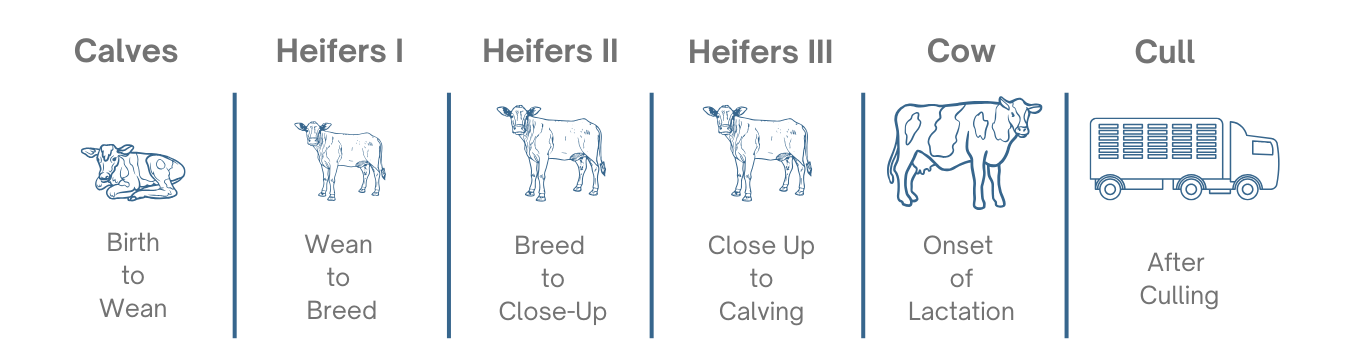
\includegraphics[width=0.9\textwidth]{resources/animalgroups.png} % Replace with your image file
  \caption{There are 5 life stages from calf to cow and a cull stage as outlined in this figure.}
  
\end{figure}

\textbf{Progression Between Life Stages:} Calves progress to Heifer I when their age reaches the user-defined input for weaning day. Heifer I animals progress to Heifer II animals when their age reaches the user-defined input for breeding start day. Heifer II animals that successfully conceive progress to the Heifer III stage when they are close to calving. Specifically, Heifers II become Heifers III when the number of days left in their pregnancy is equal to the user-defined input for the prefresh days. When a Heifer III animal calves for the first time, she becomes a Cow and will remain a cow for the rest of her life on the RuFaS farm. 

When a Heifer III calves for the first time and becomes a Cow, then that animal will cycle through lactating and non-lactating phases until they are removed from the herd due to a failure to conceive or a user-provided probability for culling within each parity. The methods that determine when a cow will leave the herd are described in detail in the Herd Exits section.

\textbf{Parturition and New Calves: }
When a Heifer III or Cow animal reaches the end of their pregnancy and starts lactating, a new calf animal object is created and assigned a birthweight according to a user-informed random distribution. All male calves are recorded and removed from the farm on day 1 of their life. Female calves remain on the farm determined by an event-based Monte Carlo method informed by the user-defined percent of female calves that are kept. 
\subsection{RuFaS Bodyweight and Growth}

    \paragraph{Introduction} An animal’s bodyweight is initialized at birth according to a user defined normal distribution. Depending on her life stage, her bodyweight is then updated daily by adding their daily growth (commonly referred to as average daily gain), conceptus weight change, and tissue accretion and depletion associated with tissue mobilization to support lactation. The changes associated with each life stage are:
    \begin{itemize}
        \item Calves increase bodyweight by calf specific estimate for daily growth from birth to weaning.
        \item Non-pregnant heifers increase bodyweight by non-pregnant heifer specific estimate for daily growth from weaning until conception.
        \item Pregnant heifers  increase their bodyweight by the pregnant heifer specific estimate for daily growth and an estimate for conceptus growth.
        \item Cows in parity 1 and 2 increase their bodyweight according to a parity and pregnancy status specific estimate for daily growth, an estimate for conceptus growth, and an estimate for body tissue changes that occur in lactation. 
        \item Cows in parities 3 and above change their bodyweight according to estimates for conceptus growth and body tissue changes that occur in lactation.
    \end{itemize}
    
    These methods are further described by \textcite{Li2023}

\textbf{Required User Inputs} 

\renewcommand{\arraystretch}{1.4}
\begin{longtable}{@{} L{4cm} L{6.5cm} L{1.5cm} L{1cm} L{1cm} @{}}
\caption{Below is a summary of the user inputs that are available and their definitions.} \\
\toprule

\multicolumn{1}{c}{\textbf{Variable}} & 
\multicolumn{1}{c}{\textbf{Definition (units)}} & 
\multicolumn{1}{c}{\textbf{Default}} & 
\multicolumn{1}{c}{\textbf{Min}} & 
\multicolumn{1}{c}{\textbf{Max}} \\

\midrule
\endfirsthead

\toprule
\multicolumn{1}{c}{\textbf{Variable}} & 
\multicolumn{1}{c}{\textbf{Definition (units)}} & 
\multicolumn{1}{c}{\textbf{Default}} & 
\multicolumn{1}{c}{\textbf{Min}} & 
\multicolumn{1}{c}{\textbf{Max}} \\
\midrule
\endhead

\bottomrule
\endfoot

\bottomrule
\endlastfoot

birth\_weight\_avg\_ho       & Average Holstein Birth Weight (kg/head)       & 42.9       & 1       & NA \\
birth\_weight\_std\_ho       & Holstein Birth Weight Standard Deviation (kg/head)       & 69       & 0       & NA \\
birth\_weight\_avg\_je       & Average Jersey Birth Weight (kg/head)       & 25.2       & 1       & NA \\
birth\_weight\_std\_je       & Jersey Birth Weight Standard Deviation (kg/head)       & 4.4       & 0       & NA \\
mature\_body\_weight\_avg       & The average mature body weight of cows (kg/head)      & 740.1       & 0       & NA \\
mature\_body\_weight\_std       & The standard deviation of mature body weight of cows  (kg/head)    & 73.5       & 0       & NA \\
wean\_day       &  The days of age at which calves are fully weaned from milk or milk replacer (days)     & 60       & 0       & NA \\
target\_heifer\_preg\_day       & The target age (in days) for heifers to become pregnant - for adjusting heifer body weight (days)      & 420       & NA      & NA \\
\end{longtable}

\textbf{Expected Outputs} 
\begin{itemize}
    \item herd\_statistics.avg\_cow\_body\_weight (kg): the daily average bodyweight of all cows in the herd 
    \item Pen\_[pen ID]\_[pen animal combination].avg\_BW (kg): the daily average bodyweight of all animals in each pen
    \item sold\_weight (kg)
\end{itemize}
\vspace{0.5cm}

    \paragraph{Methodology} 
    
    Most methods determining the bodyweight of animals in RuFaS are implemented in growth.py. 
    
    The function evaluate\_body\_weight\_change in growth.py calls the appropriate bodyweight change functions for each animal depending on their life stage and sums the appropriate changes into a single variable called daily\_growth. 

    After setting the daily bodyweight change in the daily\_growth variable, the evaluate\_body\_weight\_change function updates each animal's bodyweight by adding it to the current body\_weight. Thus for all animals, the final updated body\_weight is set as:
    \vspace{0.25cm}
    
    \begin{center}
    \(\text{body\_weight}_{\text{updated}} = \text{body\_weight}_{\text{current}} + \text{daily\_growth}\)        
    \end{center}

\begin{itemize}
    \item \textbf{Calf Birth Weight} is assigned in reproduction.py using a random draw from a truncated normal distribution based on user inputs for the breed-specific average and standard deviation of the birthweight. The distribution is truncated at +/- 2 SD from the mean to prevent extremely small or large calves. 
    \vspace{0.5cm}
    
\begin{center}
    \(Birth\ Weight = Random\ N\ (average\_birth\_weight\_by\_breed,\ std\_std\_birth\_by\_breed)\) 
    
    *Note - truncated at 2 standard deviations
\end{center}
    \vspace{0.5cm}
    
    {\raggedleft \textbf{[AN.BWT.6]}\par}
    \vspace{0.5cm}

    \item \textbf{Calf Growth} Calves are assumed to double their weight between birth and weaning based on recommendations in the \cite{nrc2001}. Thus the target average daily gain is estimated as:
    \vspace{0.5cm}

\begin{center}
    
    \(target\_average\_daily\_gain = \frac{birth\ weight}{wean\ day}\)
    
\end{center}
    \vspace{0.5cm}
    
    {\raggedleft \textbf{[AN.BWT.7]}\par}
    \vspace{0.5cm}
    
    \item \textbf{Non Pregnant Heifer Growth} The daily growth for non-pregnant heifers is estimated through an average daily gain to reach 55\% of their manure bodyweight by the time they are pregnant. Because the actual age at pregnancy is not known, a user input for the target\_heifer\_preg\_day is used to estimate the target average daily growth or ADG. A minimum daily growth rate of 0.5 kg/d is enforced so if the estimated daily\_growth is less than 0.5 kg/d, the minimum value is used. 
    \vspace{0.5cm}
    
 \begin{center}
    \(target\_average\_daily\_gain = min(\frac{0.55×MSBW-SBW}{abs(target heifer pregnant age-age)}\),0.5)
\end{center}
    \vspace{0.5cm}
    
    {\raggedleft \textbf{[AN.BWT.8]}\par}
    \vspace{0.5cm}
    
    Where MSBW is mature shrunk bodyweight (0.96 x mature bodyweight) and SBW is shrunk bodyweight (0.96 x bodyweight)
    
    \item \textbf{Pregnant Heifer Growth} Heifers are targeted to grow to 82\% of their mature body weight by the time of their first calving. A gestation length is set at conception. The ADG of pregnant heifers is calculated based on the target heifer's body weight, gestation length, and days in pregnancy. The gestation length for each animal is set at conception by calculate\_gestation\_length in reproduction.py.
    \vspace{0.5cm}
 
\begin{center}
    \(target\_average\_daily\_gain = \frac{0.82×MSBW-SBW}{gestation length - days in pregnancy}\)
\end{center}
    \vspace{0.5cm}
    
    {\raggedleft \textbf{[AN.BWT.9]}\par}
    
    \item \textbf{Parity 1 and 2 Cow Growth} The daily growth of cows is calculated based on the target of reaching 92\% of the mature body weight by the end of the 1st lactation, and full mature body weight at the end of the 2nd lactation. Before pregnancy, the daily growth is estimated based on the calving interval and during pregnancy the daily growth is calculated based on days until calving. 
    \vspace{0.5cm}
    
    \paragraph{Parity 1 Animals:}
    \vspace{0.25cm}
    
    \textbf{\textit{If not pregnant:}}
    \vspace{0.5cm}
    
\begin{center}
    \(target\_average\_daily\_gain = \frac{(0.92-0.82) × MSBW}{calving\_interval}\)
\end{center}
    \vspace{0.5cm}
    
    {\raggedleft \textbf{[AN.BWT.10]}\par}
    \vspace{0.5cm}
    
    \textbf{\textit{If pregnant:}}
    \vspace{0.5cm}
    
\begin{center}
    \(target\_average\_daily\_gain = \frac{0.92 × MSBW - bodyweight}{gestation\_length - DIP}\)
\end{center}
    \vspace{0.5cm}
    
    {\raggedleft \textbf{[AN.BWT.11]}\par}
    \vspace{0.5cm}

    \paragraph{Parity 2 Animals}
    \vspace{0.5cm}

    
    \textbf{\textit{If not pregnant:}}
    \vspace{0.5cm}
    
\begin{center}
    \(target\_average\_daily\_gain = \frac{(1 - 0.92) × MSBW}{calving\_interval}\)
\end{center}
    \vspace{0.5cm}
    
    {\raggedleft \textbf{[AN.BWT.12]}\par}
    \vspace{0.5cm}
    
    \textbf{\textit{If pregnant:}}
    \vspace{0.5cm}
    
\begin{center}
    \(target\_average\_daily\_gain = \frac{(MSBW - bodyweight)}{gestation\_length - DIP}\)
\end{center}
    \vspace{0.5cm}
    
    {\raggedleft \textbf{[AN.BWT.13]}\par}
    \vspace{0.5cm}
    
The gestation length for cows is estimated with the same methods that are used for heifers and the calving interval is set either as the average herd calving interval or the animal’s own calving interval which is calculated as the age at her second calving minus her age at first calving as part of the daily\_reproduction\_update in animal.py.

    \item \textbf{Conceptus Growth} is estimated the same way for both heifers and cows using a non-linear model for animals that are greater than 50 days in pregnancy based on the methods developed by \textcite{Korver1985}. 
    \vspace{0.25cm}
    
    If the heifer or cow days in pregnancy is greater than 50  and less than the gestation length:

    First the expected total conceptus weight is estimated using an empirical equation based on the calf birth weight and the gestation length:
     \vspace{0.5cm}
     
\begin{center}
    \(conceptus\_total\_weight = (0.0148\ *\ gestation\_length) × calf\_birth\_weight\)
\end{center}
    \vspace{0.5cm}
    
    {\raggedleft \textbf{[AN.BWT.14]}\par}
    \vspace{0.5cm}
    
    Then an animal specific conceptus parameter is calculated:
     \vspace{0.5cm}
     
\begin{center}
    \(conceptus\_parameter = \frac{total\_conceptus\_weight^\frac{1}{3}}{gestation\_length - 50}\)
\end{center}
    \vspace{0.5cm}
    
    {\raggedleft \textbf{[AN.BWT.15]}\par}
    \vspace{0.5cm}
    
    Finally, the conceptus growth is estimated as:
     \vspace{0.5cm}
     
\begin{center}
    \(conceptus\_growth = 3\ *\ conceptus\ parameter^3\ *\ (DIP - 50)^2\)
\end{center}
    \vspace{0.5cm}
    
    {\raggedleft \textbf{[AN.BWT.16]}\par}
    \vspace{0.5cm}
    
    When days\_in\_pregnancy = gestation\_length and the animal calves, then conceptus growth is set to the negative value of the current conceptus\_weight such that the weight of the calf and placenta are subtracted from the cow’s bodyweight when her bodyweight is updated.
        \vspace{0.5cm}
        
\begin{center}
    \(conceptus\_growth = conceptus\_weight\)
\end{center}
    \vspace{0.5cm}
    
    {\raggedleft \textbf{[AN.BWT.17]}\par}
    \vspace{0.5cm}
    
    \item \textbf{Tissue Change Due to Lactation} Lactation related tissue changes are estimated by a non-linear model presented by \textcite{Galvao2013} that estimates the daily tissue mobilized during lactation. 
     \vspace{0.5cm}
     
\begin{center}
    \(bodyweight\_tissue\_change = \frac{P1}{P2}\ *\ exp\ (1\ -\ \frac{DIM}{P2})\ +\ DIM\ x\ exp\ (1\ -\ \frac{DIM}{P2})\)
\end{center}
    \vspace{0.5cm}
    
    {\raggedleft \textbf{[AN.BWT.18]}\par}
    \vspace{0.5cm}
    
    Where P\textsubscript{1} and P\textsubscript{2} are parameters with distinct values for primiparous and multiparous cows:

    \begin{table}[h!]
    \centering
    \renewcommand{\arraystretch}{1.3}

    \begin{tabular}{@{} L{3cm} L{3cm} L{3cm} @{}}
    \toprule
    \multicolumn{1}{c}{\textbf{Parameter}} & 
    \multicolumn{1}{c}{\textbf{Primiparous}} & 
    \multicolumn{1}{c}{\textbf{Multiparous}} \\
    \midrule
    P\textsubscript{1}    & 20   & 65 \\
    P\textsubscript{2}    & 40 & 70 \\
    \bottomrule
    \end{tabular}
    \end{table}


    During the dry period, the net tissue change is assumed to be restored during the dry period. The net tissue change is estimated on the last day of lactation as: 
    \vspace{0.5cm}
    
    \begin{center}
    \(tissue\_changed = P_1\ *\ \frac{DIMlast}{P_2}\ *\ exp\ (1\ -\ \frac{DIMlast}{P_2})\ +\ DIM\ *\ exp\ (1\ -\ \frac{DIM}{P_2})\)
    \end{center}
    \vspace{0.5cm}
    
    {\raggedleft \textbf{[AN.BWT.19]}\par}
         \vspace{0.5cm}
         
    \begin{center}
    \(bodyweight\_tissue\_change = \frac{tissue\ changed}{gestation\ length\ -\ DIPdry}\)
    \end{center}
    \vspace{0.5cm}
    
    {\raggedleft \textbf{[AN.BWT.20]}\par}
\end{itemize}

 


\subsection{Animal Reproduction} 
 
    \paragraph{Introduction} The reproduction component of the RuFaS model is designed based on reproductive program options recommended by the Dairy Cattle Reproduction Council \parencite{dcrc_protocols} and experts in the field. It offers three pre-defined reproductive program options for nulliparous heifers (estrus detection [ED], timed artificial insemination [TAI], and synchronized estrus detection [Synch-ED]) and three options for lactating cows (ED, TAI, and a combined ED-TAI approach). Users can select appropriate reproductive protocols and specify reproductive performance variables for both nulliparous heifers and lactating cows.
    
    \vspace{0.20cm}This reproduction component simulates key reproductive events, including estrus occurrence, estrus detection, hormone administration, artificial insemination (AI), pregnancy checks, and pregnancy outcomes (abortion or successful delivery). Reproductive culling decisions are also modeled, based on an animal's inability to conceive or sustain a pregnancy. These processes are modeled using Monte Carlo simulations to represent variability in reproductive events.

    \vspace{0.2cm}The simulation generates and tracks detailed reproductive performance metrics at the animal level. These outputs provide insights into estrus detection, synchronization treatments, breeding efficiency, and pregnancy outcomes. The key recorded variables include:
    \begin{itemize}
        \item Estrus Detection (ED) Metrics: Number of days an animal participates in the ED program (ED\_days) and the total estrous events detected (estrus\_count).
        \item Hormonal Treatments: Counts of synchronization protocol injections, including GnRH (GnRH\_injections), PGF (PGF\_injections), and CIDR (CIDR\_injections).
        \item Breeding Interventions: Number of semen straws used (semen\_number) and total AI procedures performed (AI\_times).
        \item Reproductive Efficiency: Time from first breeding attempt to pregnancy confirmation (breeding\_to\_pregnancy\_time) and the interval from calving to confirmed pregnancy (calving\_to\_pregnancy\_time).
        \item Pregnancy Monitoring: Total number of pregnancy checks performed (pregnancy\_diagnoses).
    \end{itemize}

\textbf{Required User Inputs}
\vspace{-0.25cm}


% --- Table 1: Heifer Reproductive Inputs ---
\begin{landscape}
\thispagestyle{empty}
\begin{table}[h!]
\caption{Below are the key user inputs that determine the \textbf{heifer reproductive breeding program} and impact reproductive efficiency and age at first calving.}
\centering
\renewcommand{\arraystretch}{1.4}
\begin{tabular}{@{} L{3.5cm} L{3cm} L{8cm} C{2cm} C{2cm} C{2cm} @{}}
\toprule
\textbf{Section} & \textbf{Variable} & \textbf{Definition} & \textbf{Default} & \textbf{Min} & \textbf{Max} \\
\midrule

\multirow{3}{*}{\textbf{management\_decisions}} 
 & breeding\_start\_day\_h & Age when RuFaS initiates estrous protocol (days) & - & 380 & 0 \\
 & heifer\_repro\_method & TAI (Timed AI), ED (Estrus Detection), Synch-ED (Synchronized ED) & TAI & \multicolumn{2}{C{6cm}}{TAI, ED, Synch-ED} \\
 & heifer\_repro\_cull\_time & Age when a heifer is culled if not pregnant (days) & - & 500 & 0 \\
\cmidrule(lr){1-6}

\multirow{5}{*}{\textbf{farm\_level\_heifers}} 
 & estrus\_detection\_rate & Proportion of estrus detected in ED protocol & 0.9 & 0 & 1 \\
 & estrus\_conception\_rate & Conception rate in ED protocol & 0.6 & 0 & 1 \\
 & repro\_sub\_protocol & Hormone protocol used; varies by method (e.g., 5dCG2P, CP, N/A) & 5dCG2P & \multicolumn{2}{C{6cm}}{5dCG2P, 5dCGP, 2P, CP, N/A} \\
 & conception\_rate & Conception rate for sub-protocol & 0.6 & 0 & 1 \\
 & estrus\_detection\_rate & Detection rate in sub-protocol & 0.6 & 0 & 1 \\
\bottomrule
\end{tabular}
\end{table}
\end{landscape}


% --- Table 2: Cow Reproductive Inputs (longtable) ---
\begin{landscape}
\thispagestyle{empty}
\renewcommand{\arraystretch}{1.4}

\begin{longtable}{@{} L{3.5cm} L{3cm} L{8cm} C{2cm} C{2cm} C{2cm} @{}}
\caption{The following inputs determine reproductive efficiency of cows and influence culling, calving interval, and calf output.} \\
\toprule
\textbf{Section} & \textbf{Variable} & \textbf{Definition} & \textbf{Default} & \textbf{Min} & \textbf{Max} \\
\midrule
\endfirsthead

\multicolumn{6}{@{}l}{\textit{Table continued from previous page}} \\
\toprule
\textbf{Section} & \textbf{Variable} & \textbf{Definition} & \textbf{Default} & \textbf{Min} & \textbf{Max} \\
\midrule
\endhead

\midrule
\multicolumn{6}{@{}r@{}}{\textit{Continued on next page}} \\
\endfoot

\bottomrule
\endlastfoot

\multirow{2}{*}{\textbf{management\_decisions}} 
& cow\_repro\_method & TAI, ED, ED-TAI protocols & TAI & \multicolumn{2}{C{6cm}}{TAI, ED, ED-TAI} \\
& do\_not\_breed\_time & Days after calving to stop breeding if not pregnant & 185 & 0 & - \\
\cmidrule(lr){1-6}

\multirow{2}{*}{\textbf{farm\_level}} 
& voluntary\_waiting \_period & Days before breeding starts for ED/ED-TAI; ignored in TAI & 50 & 0 & - \\
& estrus\_detection \_protocol & Estrous protocol type & Double OvSynch & \multicolumn{2}{C{6cm}}{Double OvSynch, PreSynch, G6G, None} \\
\cmidrule(lr){1-6}

\multirow{3}{*}{\textbf{farm\_level\_cows}} 
& estrus\_conception\_rate & Conception rate for ED/ED-TAI & 0.5 & 0 & - \\
& presynch\_program & Presynch method used in TAI & OvSynch 56 & \multicolumn{2}{C{6cm}}{OvSynch 48, OvSynch 56, CoSynch 72, 5d CoSynch, None} \\
& presynch\_program \_start\_day & Day of first hormone injection for presynch & 70 & 0 & - \\
& ovsynch\_program & OvSynch protocol used in TAI or ED-TAI & 0.6 & 0 & 1 \\
& ovsynch\_program \_start\_day & Start day for OvSynch protocol & TAIafterPD & \multicolumn{2}{C{6cm}}{TAIafterPD, TAIbeforePD, PGFatPD, None} \\
& ovsynch\_program \_conception\_rate & Conception rate for OvSynch program & - & - & - \\
& resynch\_program & Resynch protocol around pregnancy check & - & - & - \\
\end{longtable}

\vspace{-0.3cm}
{\footnotesize\textit{NOTE:} Anytime an insemination is performed after an OvSynch program, the conception rate will be changed to the ovsynch\_program\_conception\_rate.}
\end{landscape}


% --- Table 3: Conception Rate Modifiers ---
\begin{landscape}
\thispagestyle{empty}
\begin{table}[h!]
\caption{The following inputs can be used to determine if there is a \textbf{decrease in the conception rate} with parity and rebreeding attempts.}
\centering
\renewcommand{\arraystretch}{1.4}
\begin{tabular}{@{} L{2cm} L{5cm} L{8cm} C{2cm} C{2cm} C{2cm} @{}}
\toprule
\textbf{Section} & \textbf{Variable} & \textbf{Definition} & \textbf{Default} & \textbf{Min} & \textbf{Max} \\
\midrule

\multirow{3}{*}{\textbf{farm\_level}} 
& conception\_rate\_decrease & Percent decrease per breeding attempt after first & 0.026 & 0.1 & 0 \\
& decrease\_conception\_rate \_in\_rebreeding & Whether to decrease rate with rebreeding & FALSE & - & - \\
& decrease\_conception\_rate \_by\_parity & Whether to decrease rate by parity & FALSE & - & - \\
\bottomrule
\end{tabular}
\end{table}
\end{landscape}









\textbf{Relevant Outputs}

Overall reporting for reproductive measures can be summarized and split into scheduled events and updates on an individual basis for heifers and cows. 

These include: 
\begin{itemize}
    \item Events for Estrus (detection and scheduling)
    \item Hormone Administration
    \item Artificial Insemination (AI) (scheduling and status)
    \item Pregnancy Checks and Status
    \item Days Carry Calf
    \item Abortion Events
    \item Updates to Lactation
    \item Updates to Estrous
    \item Updates to Pregnancy
    \item Updates to Reproductive Status or Culling Decisions
    \item Updates to Protocols
\end{itemize}

    \paragraph{Methodology} 
    \textbf{\textit{Heifer Breeding}}
    \vspace{0.2cm}
    
    \textbf{Heifer II} - The heiferII\_reproduction\_update represents the breeding-eligible heifer stage, beginning when the animal enters a reproductive management program and ending when she reaches a user-defined day in pregnancy that marks the start of the pre-fresh period (prefresh\_day). The breeding process follows the assigned reproductive management program and is simulated as described below (Figure 2). Each program includes a user-defined conception rate (conception\_rate), determining the probability of pregnancy initiation at the time of insemination. 
    \begin{figure}[H] % The 'p' option places the figure on a page by itself
  \centering
  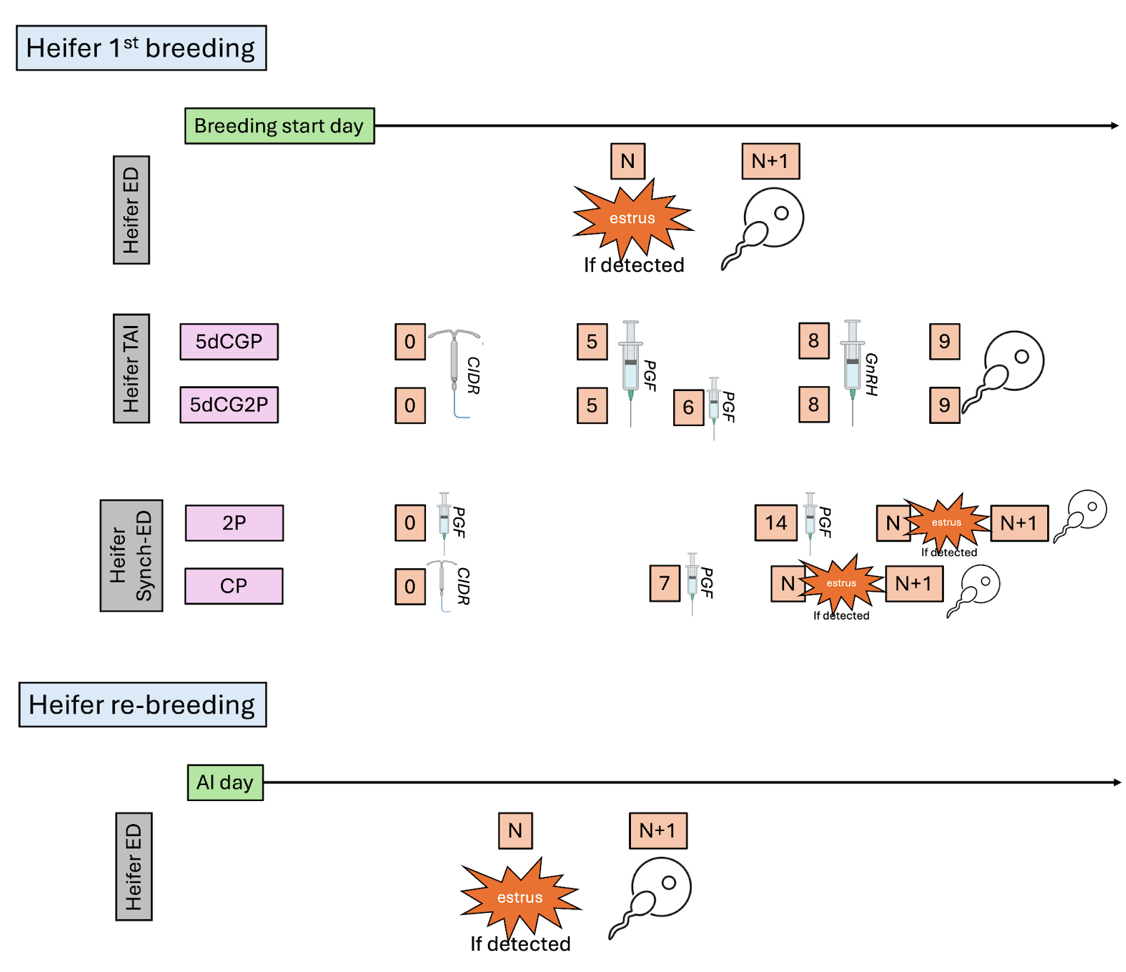
\includegraphics[width=0.7\textwidth]{resources/repromethod.png} % Replace with your image file
  \caption{This is a high level schematic to illustrate the  methodology behind the heifer breeding and re-breeding in RuFaS Animal Module.}
  
\end{figure}
    Pregnancy diagnosis and reconfirmation occur after each insemination [heifer\_pregnancy\_update]. If a heifer remains nonpregnant beyond a user-defined age threshold (heifer\_repro\_cull\_time, e.g., 500 days), she is culled due to reproductive failure. At a user-defined day in pregnancy (prefresh\_day, e.g., one month before calving), the animal either transitions to the Heifer III stage or is sold as a replacement heifer. 
    \vspace{0.2cm}
    
    The first-service reproductive management strategy for a heifer follows one of three strategies and are described in more detail below: estrus detection (ED), synchronized estrus detection (Synch-ED), or timed artificial insemination (TAI).
    \begin{enumerate}
        \item \textbf{ED [execute\_heifer\_ed\_protocol]}: The ED strategy simulates spontaneous estrous cycles. Estrous cycle length is determined using a random draw from a normal distribution \parencite{devries2006}. On the day of estrus predicted by the model, a random draw from a uniform distribution U(0,1) is compared with the estrus detection rate (estrus\_detection\_rate). If the drawn value is lower than the detection rate, AI is scheduled on that day. If estrus is not detected, the next estrus event is scheduled based on the normal estrous cycle. On the scheduled AI day, pregnancy success is determined using a random draw from a uniform distribution U(0,1), which is compared against the conception rate (conception\_rate).
        \item \textbf {Synch-ED [execute\_heifer\_synch\_ed\_protocol]}: In the Synch-ED strategy, hormonal treatment dates are scheduled according to the assigned program (repro\_sub\_protocol, 2P or CP), and estrus is simulated based on a program-specific estrous cycle following the hormonal treatment. Estrus detection and AI scheduling follow the same procedure as in the ED program. 
        \item \textbf{TAI [execute\_heifer\_tai\_protocol]}: The TAI strategy simulates hormonal treatments administered on scheduled days from the start of the synchronization protocol. The timing of treatments and AI is modeled according to the assigned specific program (5dCGP or 5dCG2P) defined as a sub-protocol in the user inputs (repro\_sub\_protocol). On the scheduled AI day, pregnancy success is determined using a random draw from a uniform distribution U(0,1), which is compared against the conception rate (conception\_rate).
    \end{enumerate}
    For all heifers who fail to conceive after the first insemination or experience pregnancy loss [open\_heifer], the ED strategy is applied for subsequent breeding attempts.
    
    \textbf{\textit{Cow Breeding}} The breeding process for cows begins after calving and the voluntary waiting period (VWP), following one of three reproductive management strategies available for cows which are similar to those described in the heifer section and are pictured in Figure 3: ED, TAI, or ED-TAI. The program assigned to a cow determines the timing of insemination and the probability of pregnancy initiation.
    \vspace{-0.5cm}

\begin{figure}[p]
  \centering
  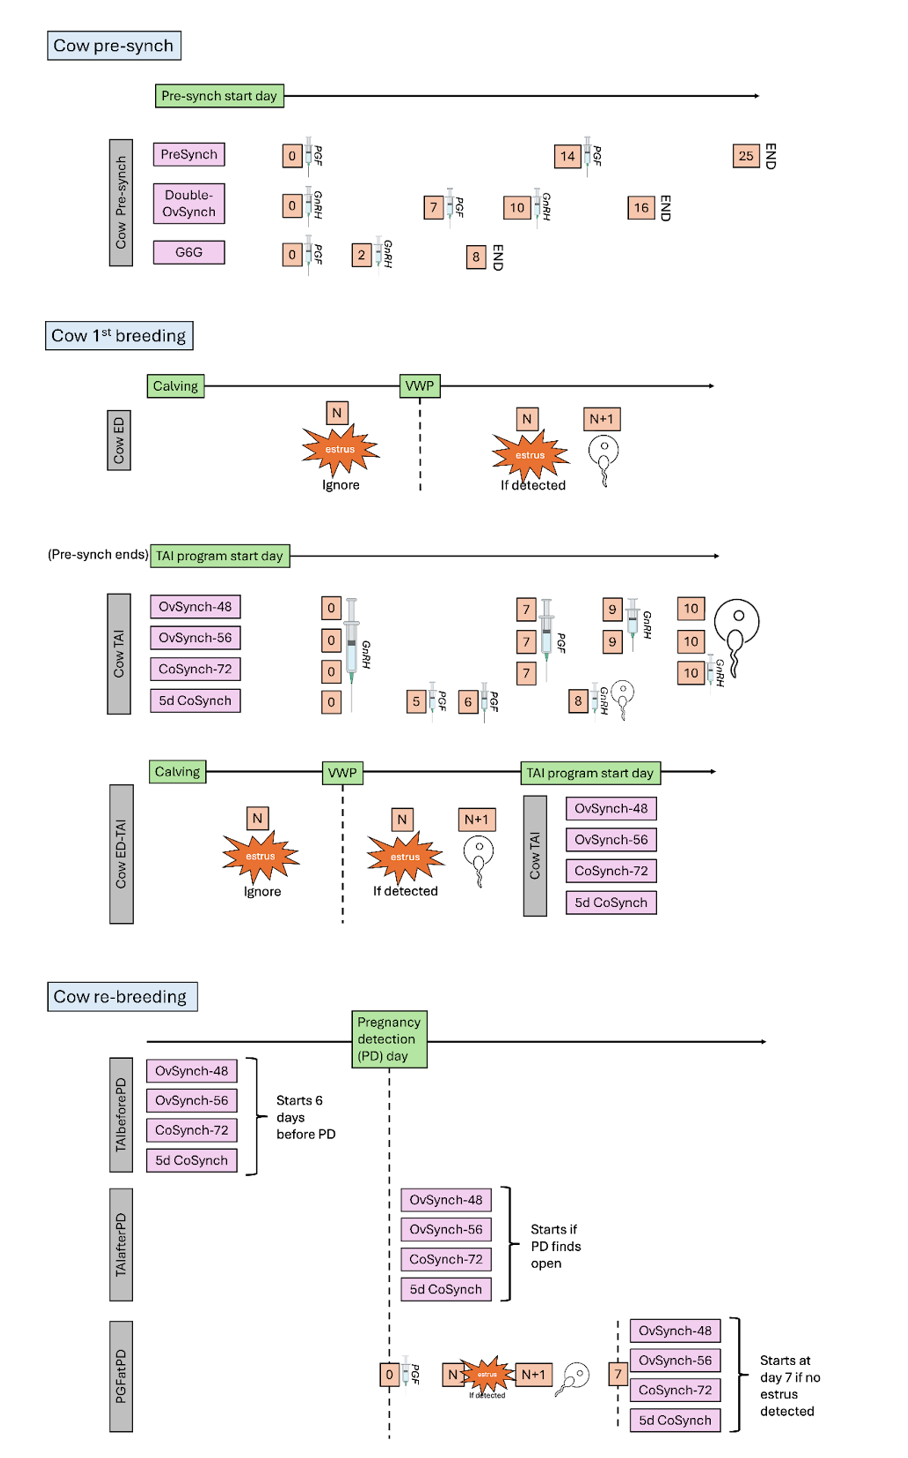
\includegraphics[width=0.75\textwidth]{resources/cowbreedmethod.png}
  \caption{This is a high level schematic to illustrate the methodology behind the cow breeding and re-breeding in RuFaS Animal Module.}

\end{figure}


    \begin{itemize}
        \item \textbf{ED [execute\_cow\_ed\_protocol]}: In the ED strategy, spontaneous estrous cycles are simulated. The first estrous cycle after calving is determined on the calving date using a random draw from a normal distribution with user-specified mean and standard deviation \parencite{kalantari2015using}. The subsequent estrous cycles are modeled similarly. If the scheduled estrus occurs before the VWP, the estrus is ignored. If the scheduled estrus occurs after the VWP, estrus detection is simulated following the same procedure as in the heifer ED strategy - a random draw from a uniform distribution U(0,1) is compared with the estrus detection rate (estrus\_detection\_rate). If the drawn value is lower than the detection rate, AI is scheduled on that day. If estrus is not detected, the next estrus event is scheduled according to the estrous cycle length. On the scheduled AI day, pregnancy success is determined using a random draw from a uniform distribution U(0,1), which is compared against the conception rate (ED\_conception\_rate). 
        \item \textbf{TAI [execute\_cow\_tai\_protocol]}: The TAI strategy simulates hormonal treatments administered on scheduled days according to the assigned synchronization protocol after the start of the breeding date (ovsynch\_program\_start\_day). The timing of treatments and AI follow the predefined protocols (ovsynch\_program, OvSynch-48, OvSynch-56, CoSynch-72, or 5d CoSynch). These protocols can be implemented alone or in combination with presynchronization protocols (presynch\_program, PreSynch, Double OvSynch, or G6G). On the scheduled AI day, pregnancy success is determined using a random draw from a uniform distribution U(0,1), compared against the conception rate.
        \item \textbf{ED-TAI [execute\_cow\_ed\_tai\_protocol]}: The ED-TAI strategy integrates ED with TAI-based synchronization programs. Estrus detection is simulated before TAI begins. If estrus is detected after VWP (voluntary\_waiting\_period) and before the initiation of the TAI (ovsynch\_program\_start\_day), AI is scheduled according to the estrus detection protocol. If no estrus is detected, the cow follows the TAI protocol for insemination.
    \end{itemize}

\begin{tcolorbox}[colback=white, colframe=black, title=Important Note]
For rebreedings, cows can be assigned to any of the three rebreeding strategies (resynch\_program, TAIbeforePD, TAIafterPD, or PGFatPD) [open\_cow].
\end{tcolorbox}


    \begin{itemize}
        \item \textbf{TAIbeforePD}: The TAIbeforePD rebreeding strategy initiates a timed AI synchronization protocol before the first pregnancy diagnosis (PD). Cows that are due for pregnancy diagnosis but have not been confirmed pregnant yet start one of the predefined synchronization protocols (OvSynch-48, OvSynch-56, CoSynch-72, or 5-day CoSynch) six days before PD. This approach ensures that if a cow is found open (not pregnant) on PD day, she is already progressing through a synchronization protocol, reducing the waiting period before the next AI attempt.
        \item \textbf{TAIafterPD}: The TAIafterPD rebreeding strategy schedules synchronization for cows that are diagnosed as open on the PD day. If a cow is not pregnant, she is immediately enrolled in one of the available timed AI protocols (OvSynch-48, OvSynch-56, CoSynch-72, or 5-day CoSynch). This ensures timely rebreeding but does not initiate synchronization in advance of PD.
        \item \textbf{PGFatPD}: The PGFatPD rebreeding strategy uses prostaglandin (PGF) administration following PD for open cows to induce estrus. After PGF treatment (day 0), cows are monitored for natural estrus. If estrus is detected, AI is performed accordingly. If no estrus is detected within seven days, the cow is enrolled in a timed AI protocol (OvSynch-48, OvSynch-56, CoSynch-72, or 5-day CoSynch) to ensure insemination. This program balances estrus detection with timed AI, allowing for natural breeding opportunities before initiating synchronization.
    \end{itemize}
    
    \vspace{1cm}
    \textbf{\textit{Pregnancy Diagnosis (PD) and Pregnancy Loss}} For both heifers and lactating cows [heifer\_pregnancy\_update, cow\_pregnancy\_update], pregnancy diagnoses are scheduled at three intervals after AI (preg\_check\_day\_1, preg\_check\_day\_2, preg\_check\_day\_3). The default settings simulate the first at 32 d after insemination, which, if confirmed positive for pregnancy, is followed at 60 d and then at 200 d \parencite{wiltbank2016}; however, the number and day of pregnancy checks can be adjusted by the model user according to farm practices. Between AI and three pregnancy checks, pregnancy losses are simulated to occur according to random draws from a U (0,1) compared with thresholds according to the expected pregnancy losses in each of those periods (preg\_loss\_rate\_1, preg\_loss\_rate\_2, preg\_loss\_rate\_3). The default values are 0.02, 0.096, and 0.017 \parencite{wiltbank2016}. Users can adjust these numbers according to their herd performance.  


\textit{On the next page are some important functions for the reproduction section of this document}


\begin{landscape}
% Suppress header/footer for all pages of the longtable
\fancypagestyle{landscapeplain}{
  \fancyhf{} % clear header and footer
  \renewcommand{\headrulewidth}{0pt}
  \renewcommand{\footrulewidth}{0pt}
}

\pagestyle{landscapeplain} % Apply to all pages in this landscape block

% Begin longtable

\thispagestyle{landscapeplain} % <-- Suppress header/footer
\textbf{\hypertarget{animfunct}{\large Reproduction Functions}} 
\vspace{0.2cm}


\renewcommand{\arraystretch}{1.4}
\begin{longtable}{@{} L{3cm}  L{7cm} L{4cm} L{4cm} L{4cm}  @{}}
\caption{Important functions for the reproduction section.} \\
\toprule

\multicolumn{1}{c}{\textbf{Function}} & 
\multicolumn{1}{c}{\textbf{Description}} & 
\multicolumn{1}{c}{\textbf{Parameters}} & 
\multicolumn{1}{c}{\textbf{Input Origins}} & 
\multicolumn{1}{c}{\textbf{Outputs}}  \\

\midrule
\endfirsthead

\toprule
\multicolumn{1}{c}{\textbf{Function}} & 
\multicolumn{1}{c}{\textbf{Description}} & 
\multicolumn{1}{c}{\textbf{Parameters}} & 
\multicolumn{1}{c}{\textbf{Input Origins}} & 
\multicolumn{1}{c}{\textbf{Outputs}}  \\
\midrule
\endhead

\bottomrule
\endfoot

\bottomrule
\endlastfoot

reproduction\_update &  Updates the reproductive status of all animals daily, including estrus occurrence, detection, AI scheduling, pregnancy status, and culling decisions. & day: (int) Current simulation day. animal\_list: (list) List of all animals in the herd. & day: Updated by the simulation engine. animal\_list: Provided as model input, updated dynamically. & Updated reproductive status for all animals in the herd. Scheduled events for estrus, AI, and pregnancy checks. \\
heiferII\_reproduction \_update &  Manages reproduction processes for Heifer II animals, including estrus detection, breeding attempts, and pregnancy checks. & heifer: (object) Individual Heifer II animal. & heifer: Passed from the herd's current Heifer II group. & Updated estrus, AI status, and pregnancy details for the heifer. \\
cow\_reproduction \_update &  Handles reproduction for lactating cows, including estrus detection, AI, and transitioning reproductive status. & cow: (object) Individual cow object. day: (int) Current simulation day. & cow: Passed from the herd's lactating group. day: Updated by the simulation engine. & Updated estrus, AI, pregnancy status, and culling decisions for the cow. \\
cow\_give\_birth &  Manages calving events, updates the reproductive status, and initializes the lactation process. & cow: (object) Individual cow object. day: (int) Current simulation day. & cow: Passed from the pregnant group. day: Updated by the simulation engine. & Updated lactation and reproductive status for the cow. \\
execute\_heifer \_ed\_protocol &  Executes the estrus detection protocol for heifers, simulating natural estrus occurrence and detection probability. & heifer: (object) Individual Heifer II animal. day: (int) Current simulation day. & heifer: Passed dynamically during estrus updates. day: Updated by the simulation engine. & Estrus detection and AI scheduling for the heifer. \\
execute\_heifer \_tai\_protocol &  Manages the TAI protocol for heifers, simulating hormone administration and AI scheduling. & heifer: (object) Individual Heifer II animal. protocol: (dict) User-defined TAI protocol details. & heifer: Passed dynamically during protocol execution. protocol: Provided as user input. & AI scheduling and protocol updates for the heifer. \\
execute\_heifer \_synch\_ed\_protocol &  Executes synchronized estrus detection protocol for heifers, combining hormonal synchronization and estrus detection. & heifer: (object) Individual Heifer II animal. protocol: (dict) User-defined Synch-ED protocol details. & heifer: Passed dynamically during protocol execution. protocol: Provided as user input. & Estrus detection, hormone administration, and AI scheduling for the heifer. \\
open\_heifer &  Handles open status updates for heifers, reassigning protocols or marking for culling if reproduction fails. & heifer: (object) Individual Heifer II animal. & heifer: Passed dynamically during daily updates. & Updated reproduction status or culling decision for the heifer. \\
heifer\_pregnancy \_update &  Updates pregnancy status for heifers, including pregnancy checks and abortion events. & heifer: (object) Individual Heifer II animal. day: (int) Current simulation day. & heifer: Passed dynamically during daily updates. day: Updated by the simulation engine. & Pregnancy status, days in pregnancy, or abortion event for the heifer. \\
execute\_cow \_ed\_protocol &  Executes estrus detection protocol for cows, simulating natural estrus occurrence and detection probability. & cow: (object) Individual cow object. day: (int) Current simulation day. & cow: Passed dynamically during estrus updates. day: Updated by the simulation engine. & Estrus detection and AI scheduling for the cow. \\
execute\_cow \_tai\_protocol &  Manages the TAI protocol for cows, simulating hormone administration and AI scheduling. & cow: (object) Individual cow object. protocol: (dict) User-defined TAI protocol details. & cow: Passed dynamically during protocol execution. protocol: Provided as user input. & AI scheduling and protocol updates for the cow. \\
execute\_cow \_ed\_tai\_protocol &  Executes ED-TAI protocol for cows, combining estrus detection with synchronized TAI scheduling. & cow: (object) Individual cow object. protocol: (dict) User-defined ED-TAI protocol details. & cow: Passed dynamically during protocol execution. protocol: Provided as user input. & Estrus detection, hormone administration, and AI scheduling for the cow. \\
cow\_pregnancy \_update &  Updates pregnancy status for cows, including pregnancy checks and abortion events. & cow: (object) Individual cow object. day: (int) Current simulation day. & cow: Passed dynamically during daily updates. day: Updated by the simulation engine. & Pregnancy status, days in pregnancy, or abortion event for the cow. \\
open\_cow &  Handles open status updates for cows, reassigning protocols or marking for culling if reproduction fails. & cow: (object) Individual cow object. & cow: Passed dynamically during daily updates. & Updated reproduction status or culling decision for the cow. \\


\end{longtable}

\vspace{0.5cm}
\end{landscape}


\subsection{Milk Production} 
 
    \paragraph{Introduction} This section describes how RuFaS determines the amount of milk and milk components produced by a particular cow on a particular day. 
    \vspace{0.25cm}
    
    Milk yield is largely determined by lactation curve parameters. Wood’s curve is the only lactation model implemented in RuFaS currently, but there is flexibility to potentially include other models as well. At the beginning of the simulation, the herd is assigned distributions for the Wood’s curve parameters l, m, and n for each parity of cows (see more information in the Lactation Curve section). At the beginning of each new lactation, each cow is assigned a set of parameters for that lactation based on the herd’s distributions for her current parity. 
    \vspace{0.25cm}
    
    When the cow starts lactating, she produces milk from the calving day until dry or culled according to the assigned lactation curve model. Each day, each cow’s milk production is calculated and recorded. Milk production is calculated from the Wood’s curve equation using the given lactation curve parameters and days in milk, and then adjusted by applying random variation and any milk reduction required by other parts of the model. Milk components (protein, fat, and lactose) are calculated based on milk production and percent of each component for each cow. 
    \vspace{0.25cm}
    
    Currently, the only source of milk reduction is if there is no possible ration using the feeds available that would support the baseline level of milk production. Ration formulation is attempted with reduced milk production levels until reaching an acceptable ration (that meets the nutrient requirements for the pen’s average cow) or reaching a threshold (floor) milk production defined by some combination of user inputs and pre-defined constants. 
    



\begin{landscape}
% Suppress header/footer for all pages of the longtable
\fancypagestyle{landscapeplain}{
  \fancyhf{} % clear header and footer
  \renewcommand{\headrulewidth}{0pt}
  \renewcommand{\footrulewidth}{0pt}
}

\pagestyle{landscapeplain} % Apply to all pages in this landscape block

\textbf{ Required User Inputs}
\vspace{0.2cm}


\renewcommand{\arraystretch}{1.4} % More vertical space between rows

\begin{longtable}{@{} L{4cm} L{4cm} p{7cm} C{2cm} C{3cm} C{3cm} @{} }

\caption{The following user inputs are used to estimate customized herd-level lactation curve parameters. See the Methodology section of this document and the Lactation Curve Scientific Documentation for more detail about how these inputs are used with relation to daily milk production.} \\
\toprule
\multicolumn{1}{c}{\textbf{Section}} & 
\multicolumn{1}{c}{\textbf{Variable}} & 
\multicolumn{1}{c}{\textbf{Definition}} & 
\multicolumn{1}{c}{\textbf{Default}} & 
\multicolumn{1}{c}{\textbf{Min}} & 
\multicolumn{1}{c}{\textbf{Max}} \\
\midrule
\endfirsthead

\multicolumn{6}{@{}l}{\textit{Table continued from previous page}} \\
\toprule
\multicolumn{1}{c}{\textbf{Section}} & 
\multicolumn{1}{c}{\textbf{Variable}} & 
\multicolumn{1}{c}{\textbf{Definition}} & 
\multicolumn{1}{c}{\textbf{Default}} & 
\multicolumn{1}{c}{\textbf{Min}} & 
\multicolumn{1}{c}{\textbf{Max}} \\
\midrule
\endhead

\midrule
\multicolumn{6}{@{}r@{}}{\textit{Continued on next page}} \\
\endfoot

\bottomrule
\endlastfoot


\multirow{2}{*}{\textbf{config \_properties }} 
& end\_date & The year and Julian day on which the simulation will end & 2009:100 & - (cutoff at 2006) & – (cutoff at 2016) \\
& FIPS\_county\_code & Unique 5-digit code that represents a specific US county & - & 1000 & 56045 \\
\cmidrule(lr){1-6}

\multirow{3}{*}{\textbf{animal \_properties }} 
& cow\_times\_milked\_per\_day & Number of Milkings (per day) -- The average or most common number of times cows are milked per day (1, 2, or 3 times daily) & 3 & 0 & - \\
& parity\_fractions & Fractions of the milking animal population that are parity 1, 2, and 3 and beyond. The sum of these fractions must be 1.0 & 1: 0.346; 2: 0.272; 3: 0.379 & 1 & 0 \\
& annual\_milk\_yield & The total milk yield generated by the farm in one year (kg). If this information is not available, it can be input as null & null & - & 0 \\
\cmidrule(lr){1-6}
lactation\_properties& milking\_cow\_fraction & Fraction of cows assumed to be in milk at any given time & 0.8365 (305/365) & 1 & 0 \\


\end{longtable}
\vspace{-0.3cm}

\end{landscape}



\begin{landscape}
\thispagestyle{empty}  % Suppress headers and footers only on this page

\renewcommand{\arraystretch}{1.4}
\begin{longtable}{@{} L{4cm} L{4cm} p{7cm} C{2cm} C{3cm} C{3cm} @{}}
\caption{The following inputs are used to determine the milk fat and milk protein percentages for each lactating cow} \\
\toprule
\textbf{Section} & 
\textbf{Variable} & 
\textbf{Definition} & 
\textbf{Default} & 
\textbf{Min} & 
\textbf{Max} \\
\midrule
\endfirsthead

\multicolumn{6}{@{}l}{\textit{Table continued from previous page}} \\
\toprule
\textbf{Section} & 
\textbf{Variable} & 
\textbf{Definition} & 
\textbf{Default} & 
\textbf{Min} & 
\textbf{Max} \\
\midrule
\endhead

\midrule
\multicolumn{6}{@{}r@{}}{\textit{Continued on next page}} \\
\endfoot

\bottomrule
\endlastfoot

\multirow{2}{*}{\textbf{animal\_properties}} 
& milk\_fat\_percent & The average or most common milk fat percentage in cow milk & 3.5 & 0 & \\
& milk\_protein\_percent & The average or most common milk protein percentage in cow milk & 3.2 & 0 & \\

\end{longtable}

\vspace{-0.3cm}


\end{landscape}






\begin{landscape}
\thispagestyle{empty}  % Suppress header and footer on this landscape page

\renewcommand{\arraystretch}{1.4} % More vertical space between rows
\begin{longtable}{@{} L{4cm} L{4cm} p{7cm} C{2cm} C{3cm} C{3cm} @{}}
\caption{The following inputs are used to constrain how much an average cow’s daily milk production will be reduced due to an inadequate ration. See the Methodology section of this document and the Ration Formulation scientific documentation for more detail about how these inputs are used with relation to daily milk production.} \\
\toprule
\multicolumn{1}{c}{\textbf{Section}} & 
\multicolumn{1}{c}{\textbf{Variable}} & 
\multicolumn{1}{c}{\textbf{Definition}} & 
\multicolumn{1}{c}{\textbf{Default}} & 
\multicolumn{1}{c}{\textbf{Min}} & 
\multicolumn{1}{c}{\textbf{Max}} \\
\midrule
\endfirsthead

\multicolumn{6}{@{}l}{\textit{Table continued from previous page}} \\
\toprule
\multicolumn{1}{c}{\textbf{Section}} & 
\multicolumn{1}{c}{\textbf{Variable}} & 
\multicolumn{1}{c}{\textbf{Definition}} & 
\multicolumn{1}{c}{\textbf{Default}} & 
\multicolumn{1}{c}{\textbf{Min}} & 
\multicolumn{1}{c}{\textbf{Max}} \\
\midrule
\endhead

\midrule
\multicolumn{6}{@{}r@{}}{\textit{Continued on next page}} \\
\endfoot

\bottomrule
\endlastfoot

\multirow{2}{*}{\textbf{feed\_properties}} 
& milk\_reduction\_maximum & Allowable amount of milk reduction (kg) when dietary nutrient supply cannot meet animal requirements &     &   0 & 50 \\

& tolerance & Allowable +/- percentage variance in each of the defined ration inclusion percentage values. 

\textit{This variable defaults to 0.0 and currently has no effect due to no implementation of an automatic ration optimizer. RuFaS is hard-coded to use the user-defined ration at this time.}
  & 0 & 0 & 1 \\

\end{longtable}

\end{landscape}



\textbf{Relevant Outputs}
\vspace{-0.25cm}

    \begin{itemize}
        \item report\_life\_cycle\_manager\_data:	
        \begin{itemize}
            \item Information added daily from herd statistics
            \item daily\_milk\_production 
            \item herd\_milk\_fat\_percent
            \item herd\_milk\_fat\_kg
            \item herd\_milk\_protein\_percent 
            \item herd\_milk\_protein\_kg
        \end{itemize}

        \item report\_average\_nutrient\_requirements: 
        \begin{itemize}
            \item Reports the average ration per animal of each pen each time a new ration is formulated 
            \item avg\_milk\_production\_reduction\_pen (kg per animal)
        \end{itemize}
    \end{itemize}


    \paragraph{Methodology}
    \begin{enumerate}

        \item \textbf{\textit{Herd Level Lactation Curve Parameters}} 
        \vspace{0.1cm}
        
        At the beginning of the simulation, the herd is assigned distributions for the lactation curve parameters l, m, and n for each parity of cows. It calculates Wood’s lactation curve parameter mean values by parity, adjusted based on the location, production, management practices, +/- reported milk production of the farm being simulated. 
         \vspace{0.1cm}

         \textit{User Inputs and Constants}
         \vspace{0.1cm}

         The following inputs are used to generate the herd’s values for mean lactation curve parameters by parity. 
            
         \begin{itemize}
             \item year: end\_date in the input config.json. Uses 2016 if the end year is 2016 or later.  
             \item region: assigns the appropriate region based on FIPS\_county\_code entered in the input config.json  
             \item milking frequency: cow\_times\_milk\_per\_day in input animal.json 
             \item parity distribution: parity\_fractions in input animal.json 
             \item annual milk yield (optional): annual\_milk\_yield in animal.json 
             \item Milking\_cow\_fraction: 0.8356 default value 
             \begin{itemize}
                 \item Is in lactation\_curve\_adjustment\_inputs.json 
                 \item Fraction of lactating cows in adult cows, between 0 and 1. 
                 \item Used to calculate adjusted lactation curve parameters to match a herd’s reported annual milk production 
             \end{itemize}
         \end{itemize}
         
         \textit{Parameters and Equations}
         \vspace{0.1cm}

         These are comprehensively outlines in the Lactation Curve Parameters Determination Section.
        \vspace{0.1cm}
        
         LactationCurve.set\_lactation\_parameters() is called by:
         \begin{itemize}
             \item HerdFactory.initialize\_herd() to Animal.setup\_lactation\_curve\_parameters() 
             \item HerdManager.\_init\_() 

         \end{itemize}
        \vspace{0.2cm}
        
        \item \textbf{\textit{Cow Level Lactation Curve Parameters}} 
        \vspace{-0.1cm}
        
        Each cow is assigned a set of parameters for each lactation based on the herd’s distributions of l, m, and n for her current parity. This occurs when a cow is initialized at the beginning of the simulation, when a heiferIII (close-up heifer) transitions into a cow, and each time a cow has a calf. It selects Wood’s curve parameters for the cow for each parameter for each parity from the distributions based on the means calculated for the herd and constant standard deviations.
         \vspace{0.1cm}

         \textit{User Inputs and Constants}
         \vspace{0.1cm}

         No additional inputs to consider. 
         
         \textit{Parameters and Equations}
         \vspace{0.1cm}

        \begin{itemize}
            \item LactationCurve.get\_wood\_parameters() is called by
            \begin{itemize}
                \item Animal.\_initialize\_cow
                \item Animal.daily\_reproduction\_update
                \item Animal.transition\_heiferIII\_to\_cow
            \end{itemize}
            \item Parity groupings are as follows: 1, 2, and 3+ 
            \item Immediately followed in each case by self.milk\_production.set\_wood\_parameters() which assigns the l, m, and n values.
        \end{itemize}
            \vspace{0.25cm}

        \item \textbf{\textit{Daily Milk Production}} 
        \vspace{0.1cm}
        
        Each day, each cow’s milk production is calculated and recorded. Milk production is calculated from the Wood’s curve equation using the given lactation curve parameters and days in milk. The calculated production is then adjusted by applying random variation and any milk reduction required by other parts of the model. 
         \vspace{0.1cm}

         \textit{User Inputs and Constants}
         \vspace{0.1cm}

         No additional inputs to consider but constants are below: 
        \begin{itemize}
            \item DAILY\_MILK\_VARIATION\_MEAN: 0 kg/d
            \item DAILY\_MILK\_VARIATION\_STD\_DEV: 1.0 kg/d 
        \end{itemize}

         \textit{Parameters and Equations}
         \vspace{0.1cm}

    \begin{center}
\(Calculated\ milk\ production = l*t^m *e^{[-nt]}\)
    \end{center}
        \vspace{0.5cm} 
    
            {\raggedleft \textbf{[AN.MLK.9]}\par}
            \vspace{0.2cm}

        \begin{itemize}
            \item l, m, n = lactation curve parameters
            \item t = DIM
        \end{itemize}
        \vspace{0.2cm}

        \begin{tcolorbox}[colback=white, colframe=black, boxrule=0.5pt, arc=3pt, width=\textwidth]
            Adjusted milk production = maximum of (calculated milk production + milk production variance - milk production reduction) or 0.
        \end{tcolorbox}
        \vspace{0.2cm}

        \begin{itemize}
            \item MilkProduction.calculate\_daily\_milk\_production()
            \begin{itemize}
                \item \textbf{Called by} HerdManager.daily\_routines() to Animal.daily\_routines() to MilkProduction.perform\_daily\_milking\_update()
                \item \textbf{Parameters} 
                \begin{itemize}
                    \item Days\_in\_milk: Argument supplied from MilkProductionInputs (updated in Animal.daily\_routines)
                    \item L\_param, m\_param, n\_param: Wood\_l, wood\_m, wood\_n supplied as arguments and assigned to individual on the day of calving via set\_wood\_parameters()
                \end{itemize}
                \item \textbf{Returns} calculated milk yield on the provided day in kg 
            \end{itemize}
            \item MilkProduction.daily\_milk\_produced()
            \begin{itemize}
                \item \textbf{Inputs}
                \begin{itemize}
                    \item \_Daily\_milk\_produced (calculated above) 
                    \item Milk\_production\_variance is generated based on the mean and standard deviation for daily milk variation (stored as constants in AnimalModuleConstants)
                    \item Milk\_production\_reduction 
                \end{itemize}
            \end{itemize}
            \item \textbf{Returns} adjusted\_milk\_production (unless the milk yield calculated above was 0, in which case it returns 0)

        \end{itemize}
            \vspace{0.2cm}


        \item \textbf{\textit{Daily Components Production}} 
        \vspace{0.1cm}
        
        Milk components (true protein, fat, and lactose) are calculated daily based on that day’s milk production and percent of each component. 
        \vspace{0.1cm}
        
         \textit{User Inputs and Constants}
         \vspace{0.1cm}

         \begin{itemize}
             \item milk\_fat\_percent – single constant value for all cows in the herd 
             \item milk\_protein\_percent – single constant value for all cows in the herd 
             \item AnimalModuleConstants.MILK\_LACTOSE, current value 4.85

         \end{itemize}

         \textit{Parameters and Equations}
         \vspace{0.1cm}

        \begin{itemize}
            \item \(Daily\ nutrient\ amount\ in\ milk = milk\ production * nutrient\ percentage * 0.01\)
            \item MilkProduction.\_calculate\_nutrient\_content()
            \begin{itemize}
                \item \textbf{Called by} HerdManager.daily\_routines() to Animal.daily\_routines() to MilkProduction.perform\_daily\_milking\_update()
                \item \textbf{Parameters} 
                \begin{itemize}
                    \item Days\_milk\_produced as calculated in the Daily Milk Production section above
                    \item Nutrient\_percentage: cow’s percent true protein, fat, or lactose for each of the respective calculations
                \end{itemize}
                \item \textbf{Returns} Amount of a given nutrient in milk in kg
            \end{itemize}
        \end{itemize}
         
        \begin{tcolorbox}[colback=white, colframe=black, boxrule=0.5pt, arc=3pt, width=\textwidth]
            Please note that currently, true protein is the only milk protein currently used by the model. .
        \end{tcolorbox}

        \item \textbf{\textit{Milk Production and Reduction}} \hypertarget{myprodred}{ }
        \vspace{0.1cm}
        
        Currently, the only source of milk reduction is if there is no possible ration using the feeds available that would support the baseline level of milk production. 
        
        Each time the ration is formulated, the nutrition requirements of the pen are calculated and used to determine the ration given to each animal. The ration is checked against the nutrition requirements of the pen. If the pen contains lactating cows and the ration does not meet the average cow’s requirements, then each cow’s milk production is reduced until one of three conditions is met: 
        \begin{itemize}
            \item The ration meets the animal’s requirement (i.e. no additional reduction).
            \item The milk production of every animal is reduced by the maximum allowed (a user-defined value with default of 0.5 kg/head/d). Then the final ration and milk reduction values are used.
            \item The average milk production of the pen falls below the minimum allowable average milk production. Then the final ration and milk reduction values are used.
        \end{itemize}
        \vspace{0.2cm}
        

        \begin{figure}[H] % The 'p' option places the figure on a page by itself
            \centering
            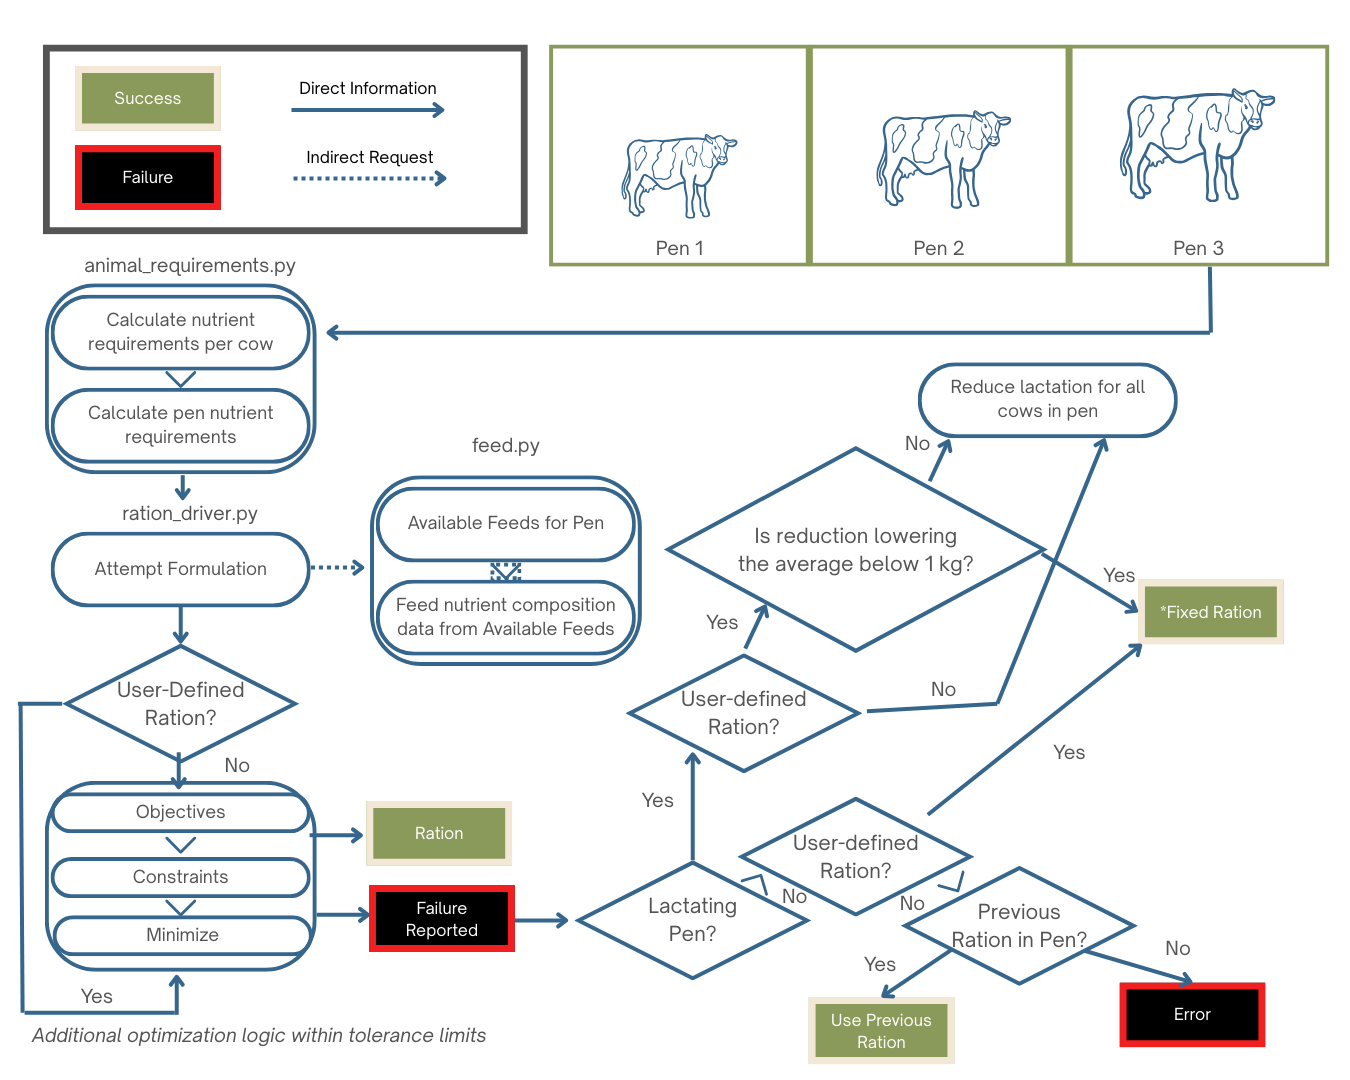
\includegraphics[width=0.9\textwidth]{resources/milkrationform.png} % Replace with your image file
            \caption{A schematic illustrating the flow of milk reduction in ration formulation logic.}
        \end{figure}
        \vspace{0.2cm}

         \textit{User Inputs and Constants}
         \vspace{0.1cm}

         \begin{itemize}
             \item Milk\_reduction\_maximum: Allowable amount of milk reduction (kg) when dietary nutrient supply cannot meet animal requirements 
             \item Tolerance: Allowable +/- percentage variance in each of the defined ration inclusion percentage values. This variable is default to 0.0 and it currently has no effect due to no implementation of automatic ration optimizer. 
            \item Milk\_reduction\_kg is set to 0.25 kg: Milk reduction amount for each failed ration attempt, kg. 
            \item Minimum\_avg\_pen\_milk is set to 15 kg: Minimum allowable average milk production, for a given pen, as used in ration formulation, kg/animal
         \end{itemize}

         \textit{Parameters and Equations}
         \vspace{0.1cm}

        \begin{itemize}
            \item Pen.reduce\_milk\_production()
            \begin{itemize}
                \item \textbf{Called by} Pen.use\_user\_defined\_ration() when NutritionEvaluator determines that the ration is inadequate to support milk production
                \item Attempts to reduce the milk production of all animals in the pen; returns False if all animals have already reached their maximum 
            \end{itemize}
            \item Animal.reduce\_milk\_production() 
            \begin{itemize}
                \item \textbf{Called by} Pen.reduce\_milk\_production for each animal in the pen 
                \item Attempts to reduce milk production of an animal in a pen; returns True if reduction was successful and False otherwise. When reduction is successful, increments milk\_production\_reduction by the value 
            \end{itemize}
        \end{itemize}


        \begin{tcolorbox}[colback=white, colframe=black, boxrule=0.5pt, arc=3pt, width=\textwidth]
            Currently, all cows in a pen will have the same milk reduction amount. This function allows future flexibility if desired to have individual reductions rather than applying the average..
        \end{tcolorbox}


        \item \textbf{\textit{Starting and Ending Lactation}} 
        \vspace{0.1cm}
    
    \textbf{Starting Lactation [Animal.transition\_heiferIII\_to\_cow]}: When a heifer reaches the point where her days pregnant is equal to gestation length, she is transitioned to a lactating cow and configuration data for a newborn calf is returned. 
    
    
    \textbf{[Reproduction.cow\_give\_birth]} and \textbf{[Animal.daily\_reproduction\_update]} When a cow’s days pregnant is equal to gestation length, she gives birth and a newborn calf is born. Her parity is incremented plus one, her days in milk is reset to 1, and she is assigned new Wood’s curve parameters for the new lactation. 
    \vspace{0.5cm}




        \begin{tcolorbox}[colback=white, colframe=black, boxrule=0.5pt, arc=3pt, width=\textwidth]
            For more information, refer to the Reproduction section of this document.
        \end{tcolorbox}
        \vspace{0.2cm}
    
    \textbf{Ending Lactation [ MilkProduction.perform\_daily\_milking\_update]}: When a cow’s days pregnant is equal to her dry off days of pregnancy, her milk production and days in milk are set to 0 and remain there until completing her gestation. Cows with days\_in\_milk = 0 are considered not to be milking and do not have any milk production values calculated. 
    \vspace{0.2cm}
            
        \begin{tcolorbox}[colback=white, colframe=black, boxrule=0.5pt, arc=3pt, width=\textwidth]
            For more details on milk changes and reductions, go to the Milk Production and Reduction portion of this section. . 
        \end{tcolorbox}
    
   
    \end{enumerate}

 
\subsection{Lactation Curve: Parameters and Definitions} 
 
    \paragraph{Introduction} The Lactation Curve Parameter Determination module calculates and adjusts Wood’s lactation curve parameters (l, m, n) based on farm-specific attributes such as geographic location, management practices, and production levels. These parameters shape the milk production curve for cows across different parities (1st, 2nd, 3rd + lactations).
    
    This module is part of the Animal Module and integrates with the Milk Production calculations. The outputs influence various downstream models, including nutrient requirements, manure excretion, and greenhouse gas emission calculations.
    
    The primary class in this module is:
    
    LactationCurve: Manages and adjusts Wood’s lactation curve parameters.

\textbf{\hypertarget{lactcurvreqinputs}{Required User Inputs}}
\vspace{-0.25cm}

% Begin longtable
 The module retrieves input data from simulation configuration files and the Input Manager. These inputs are organized into groups based on their functional roles. Each input is detailed by its parameter name, definition (including units where applicable), and any default values or constraints. There are three categories on inputs that should be considered in this section: 
 \begin{enumerate}
     \item \hyperlink{woodscurve}{Wood's Lactation Curve Base Parameters}
     \item \hyperlink{lactcurvadjust}{Adjustment Factors}
     \item \hyperlink{farmspec305}{Farm Specific 305 d Milk Production}
 \end{enumerate}
 \vspace{0.1cm}

\newpage
\begin{landscape}

% Section header
\textbf{ \hypertarget{woodscurve}{\large Lactation Curve Parameters and Inputs}} 

% Suppress header/footer for all pages of the longtable
\fancypagestyle{landscapeplain}{
  \fancyhf{} % clear header and footer
  \renewcommand{\headrulewidth}{0pt}
  \renewcommand{\footrulewidth}{0pt}
}
\pagestyle{landscapeplain}

\begin{center}
\captionof{table}{Wood's Lactation Curve Base Parameters – These inputs provide the baseline values and variability for Wood’s lactation curve parameters as derived from \textcite{Li2022}.}
\end{center}

\renewcommand{\arraystretch}{1.4} % More vertical space between rows
\begin{longtable}{@{} L{4cm} L{8cm} C{2cm} L{4cm} @{} }

\toprule
\multicolumn{1}{c}{\textbf{Variable}} & 
\multicolumn{1}{c}{\textbf{Definition}} & 
\multicolumn{1}{c}{\textbf{Units}} & 
\multicolumn{1}{c}{\textbf{Default}}  \\
\midrule
\endfirsthead

\multicolumn{4}{@{}l}{\textit{Table continued from previous page}} \\
\toprule
\multicolumn{1}{c}{\textbf{Variable}} & 
\multicolumn{1}{c}{\textbf{Definition}} & 
\multicolumn{1}{c}{\textbf{Units}} & 
\multicolumn{1}{c}{\textbf{Default}}  \\
\midrule
\endhead

\midrule
\multicolumn{4}{@{}r@{}}{\textit{Continued on next page}} \\
\endfoot

\bottomrule
\endlastfoot

parameter\_l\_mean & Baseline value for parameter $l$ of Wood’s lactation curve & Unitless & 19.9 \\
parameter\_m\_mean & Baseline value for parameter $m$ of Wood’s lactation curve & Unitless & 0.247 \\
parameter\_n\_mean & Baseline value for parameter $n$ of Wood’s lactation curve & Unitless & 0.003376 \\
parameter\_l\_std\_dev & Standard deviation for parameter $l$ & Unitless & Parity 1: 0.28; Parity 2: 0.54; Parity 3+: 0.51 \\
parameter\_m\_std\_dev & Standard deviation for parameter $m$ & Unitless & Parity 1: 0.0046; Parity 2: 0.0064; Parity 3+: 0.0060 \\
parameter\_n\_std\_dev & Standard deviation for parameter $n$ & Unitless & Parity 1: 3.77e-5; Parity 2: 5.82e-5; Parity 3+: 5.54e-5 \\

\end{longtable}
\vspace{-0.1cm}

\end{landscape}






\newpage
\begin{landscape}


% Suppress header/footer for all pages of the longtable
\fancypagestyle{landscapeplain}{
  \fancyhf{} % clear header and footer
  \renewcommand{\headrulewidth}{0pt}
  \renewcommand{\footrulewidth}{0pt}
}
\pagestyle{landscapeplain} % Apply to all pages in this landscape block

% Section header
\textbf{\hypertarget{lactcurvadjust}{\large Lactation Curve Adjustment Factors}} 

\begin{center}
    \captionof{table}{Adjustment Factors – These factors adjust the base parameters based on geographical, temporal, management, and parity considerations.}
\end{center}

\renewcommand{\arraystretch}{1.4} % More vertical space between rows
\begin{longtable}{@{} L{4cm} L{8cm} C{2cm} L{4cm} @{} }

\toprule
\multicolumn{1}{c}{\textbf{Variable}} & 
\multicolumn{1}{c}{\textbf{Definition}} & 
\multicolumn{1}{c}{\textbf{Units}} & 
\multicolumn{1}{c}{\textbf{Default}}  \\
\midrule
\endfirsthead

\multicolumn{4}{@{}l}{\textit{Table continued from previous page}} \\
\toprule
\multicolumn{1}{c}{\textbf{Variable}} & 
\multicolumn{1}{c}{\textbf{Definition}} & 
\multicolumn{1}{c}{\textbf{Units}} & 
\multicolumn{1}{c}{\textbf{Default}}  \\
\midrule
\endhead

\midrule
\multicolumn{4}{@{}r@{}}{\textit{Continued on next page}} \\
\endfoot

\bottomrule
\endlastfoot

region\_adjustments & Regional adjustments based on FIPS codes (`fips\_code`) in the configuration file & Unitless & – \\
year\_adjustments & Yearly adjustments based on calving year, defined by simulation time period (`time.end\_date.year`) & Unitless & 2006–2016 \\
milking\_frequency \_adjustments & Adjustments based on milking frequency (`cow\_times\_milked\_per\_day`) in the animal input file & Unitless & 2 or 3 \textit{\small (Classified as twice-daily (\(<\) 2.5 milkings/day) or thrice-daily ($\geq$ 2.5 milkings/day))} \\
parity\_adjustments & Adjustments to lactation curve based on parity (first, second, third+) & Unitless & 1–3 \\

\end{longtable}
\vspace{-0.1cm}

\end{landscape}


\newpage
\begin{landscape}
\thispagestyle{empty}  % Suppress header and footer on this landscape page

\textbf{\hypertarget{farmspec305}{\large Farm Specific 305-Day Milk Production Inputs}}

\renewcommand{\arraystretch}{1.4} % More vertical space between rows
\begin{longtable}{@{} L{4cm} L{8cm} C{2cm} L{4cm} @{}}
\caption{Farm Specific 305-Day Milk Production — These inputs help tailor the lactation curve to the farm’s production targets and herd composition.} \\
\toprule
\textbf{Variable} & \textbf{Definition} & \textbf{Units} & \textbf{Default} \\
\midrule
\endfirsthead

\multicolumn{4}{@{}l}{\textit{Table continued from previous page}} \\
\toprule
\textbf{Variable} & \textbf{Definition} & \textbf{Units} & \textbf{Default} \\
\midrule
\endhead

\midrule
\multicolumn{4}{@{}r@{}}{\textit{Continued on next page}} \\
\endfoot

\bottomrule
\endlastfoot

parity\_fractions & Fraction of cows by lactation parity & Fraction & Parity 1: 0.346; Parity 2: 0.272; Parity 3+: 0.379 \\
annual\_milk\_yield & Target annual milk yield to fit the lactation curve & kg & User-defined, default: null \\
milking\_cow\_fraction & Fraction of cows that are milking & Fraction & 0.8365 (User-defined) \\

\end{longtable}

\vspace{-0.1cm}
\end{landscape}



\textbf{Relevant Outputs}
\vspace{-0.25cm}

\renewcommand{\arraystretch}{1.4}
\begin{longtable}{@{} L{2cm} L{2cm} L{4cm}  @{}}
\caption{Summary of important functions for the reproduction section. } \\


\toprule
\multicolumn{1}{c}{\textbf{Parameter}} & 
\multicolumn{1}{c}{\textbf{Unit}} & 
\multicolumn{1}{c}{\textbf{Description}}  \\

\midrule
\endfirsthead

\toprule
\multicolumn{1}{c}{\textbf{Parameter}} & 
\multicolumn{1}{c}{\textbf{Unit}} & 
\multicolumn{1}{c}{\textbf{Description}}  \\
\midrule
\endhead

\bottomrule
\endfoot

\bottomrule
\endlastfoot

l & Unitless & Farm-specific scaling factor of the lactation curve by parity.  \\
m & Unitless & Farm-specific rate of milk yield increase post-calving by parity.  \\
n & Unitless & Farm-specific rate of milk yield decline after peak lactation by parity.  \\


\end{longtable}
\vspace{0.5cm}



\paragraph{Methodology} 
\vspace{0.5cm}

    \begin{enumerate}
    
        \item Determining Base Lactation Curve Parameters (set\_lactation\_parameters). The Wood’s lactation curve parameters are initialized with base values retrieved from lactation\_inputs["parameter\_mean\_values"] in LACTATION\_CURVE\_ADJUSTMENT\_INPUTS.json.
    \vspace{0.25cm}

    
        \item Adjusting parameters (\_calculate\_adjusted\_wood\_parameters). Wood's lactation curve parameters are adjusted based on temporal, geographical, and management factors \parencite{Li2022}
        \vspace{0.2cm}
        
        Each parameter (l, m, n) is adjusted using a series of modifications:
            \begin{center}
                \[l_{adjusted} = l + \sum {adjustments}\]
            \end{center}
            \vspace{0.5cm}
            
            {\raggedleft \textbf{[AN.MLK.1]}\par}
            \vspace{0.5cm}
            
            \begin{center}
                \[m_{adjusted} = m + scaling factor_{m} * \sum {adjustments}\]
            \end{center}
            \vspace{0.5cm}
            
            {\raggedleft \textbf{[AN.MLK.2]}\par}
            \vspace{0.5cm}
            
            \begin{center}
                \[n_{adjusted} = n + scaling\ factor_{n}* \sum {adjustments}\]
            \end{center}
            \vspace{0.5cm}
            
            {\raggedleft \textbf{[AN.MLK.3]}\par}
            \vspace{0.5cm}

        
        \textbf{Where:} 
            \begin{center}
                \[scaling\ factor_m = 10^{-2}\]
                \[scaling\ factor_n = 10^{-4}\]
            \end{center}  
            \vspace{0.2cm}
            
        Adjustments are applied based on:
        \begin{itemize}
            \item Region (using FIPS codes): \_get\_region\_adjustments 
            \item Year of simulation (adjusted for trends in milk production): \_get\_year\_adjustments
            \item Milking frequency (twice vs. thrice daily): \_get\_milking\_frequency\_adjustments
            \item Parity (different lactation curves for different parities): animal\_parity
        \end{itemize}

        
        \item Fitting Parameters to Target Milk Yield (\_adjust\_lactation\_curve\_to\_milk\_yield). If annual\_milk\_yield is provided, the l parameter is optimized to match the expected 305-day milk yield:
        
        \begin{itemize}
            \item Estimate Herd Average 305-day Milk Yield:
            \vspace{0.5cm}
            
            \begin{center}
                \(Milk\ Yield_{305} = \frac{Annual\ Milk\ Yield}{Number\ of\ Milking\ Cows} * \frac{305}{Days\ per\ Year}\)
            \end{center}
            \vspace{0.5cm}
            
            {\raggedleft \textbf{[AN.MLK.4]}\par}
            \vspace{0.5cm}

            \item Estimate Parity Specific 305-day Milk Yield: (\_estimate\_305\_day\_milk\_yield\_by\_parity)
            \vspace{0.5cm}
            
            \begin{center}
                \(M305_{Herd} = M305_{P1} * P1\% + M305_{\text{P2}} * P2\% + M305_{P3} * P3^+\%\)
            \end{center}
            \vspace{0.5cm}
            
            {\raggedleft \textbf{[AN.MLK.5]}\par}
            \vspace{0.5cm}
            
            \begin{center}
                \(M305_{P2} = M305_{P1} * 118\%\)
            \end{center}
            \vspace{0.5cm}
            
            {\raggedleft \textbf{[AN.MLK.6]}\par}
            \vspace{0.5cm}
            
            \begin{center}
                \(M305_{P3+} = M305_{P1} * 125\%\)
            \end{center}
            \vspace{0.5cm}
            
            {\raggedleft \textbf{[AN.MLK.7]}\par}
            \vspace{0.5cm}
            
            

        \begin{tcolorbox}[colback=white, colframe=black, boxrule=0.5pt, arc=3pt, width=\textwidth]
            118\% and 125\% are assumptions made based on the work by \textcite{Li2022}. 
        \end{tcolorbox}

            
            \item Fit l Parameter Using Optimization: (\_fit\_wood\_l\_param\_to\_milk\_yield). 
            The error function is defined as: (\_calculate\_305\_day\_milk\_yield\_error)
            \vspace{0.5cm}
            
            \begin{center}
                \(Error = Predicted\ MilkYield{305} - Target\ MilkYield{305} \)
            \end{center}
            \vspace{0.5cm}
            
            {\raggedleft \textbf{[AN.MLK.8]}\par}
            \vspace{0.5cm}
            
            Using Scipy's minimize function, the l parameter is iteratively adjusted to minimize this error.
        \end{itemize}
        
        \item Final Lactation Curve Parameter Mapping. Once adjustments are made, parameters are stored in:
        \vspace{0.5cm}
        
        \_parity\_to\_parameter\_mapping = {1: {"l": ..., "m": ..., "n": ...}, \\
                                            2: {"l": ..., "m": ..., "n": ...}, \\
                                            3: {"l": ..., "m": ..., "n": ...}}
                                            \vspace{0.2cm}


    \end{enumerate}

        
    Equations below are not in the LactationCurve class, but they are useful to understanding the bigger picture of how lactation curve parameter estimates are generated in RuFaS. Please see the Milk Production section for more details on these equations \parencite{Wood1967}.
    \vspace{0.5cm}

    \textbf{Wood's Lactation Curve}
    
            \begin{center}
                \(Y_t = l * t^{m} * e^{-nt}\)
            \end{center}
            \vspace{0.5cm}
            
            {\raggedleft \textbf{[AN.MLK.9]}\par}
            \vspace{0.5cm}

        \textbf{Where:}
        \vspace{0.2cm}
        
        \begin{itemize}
            \item Y(t): Daily milk yield.
            \item t: Time in days.
            \item l, m, n: Parameters adjusted for farm-specific conditions.
        \end{itemize}
    \vspace{0.5cm}

    \textbf{305-Day Milk Yield}
    
            \begin{center}
                \(\int_{l}^{305} lt^me^{-nt}dt\)
            \end{center}
            \vspace{0.5cm}
            
            {\raggedleft \textbf{[AN.MLK.10]}\par}
            \vspace{0.5cm}


\subsection{Culling} 

 
\paragraph{Introduction} This section describes the processes of animals leaving the herd in RuFaS. 
Reasons for leaving the herd are death or sale. 
\vspace{0.5cm}

Sale may occur of: 
\begin{itemize}
    \item Calves (all male calves; female calves based on keep\_female\_calf\_rate)
    \item Heifer II’s (if the heifer does not have a successful conception or pregnancy and age (days born) exceeds heifer\_repro\_cull\_time
    \item Heifer III’s (if cow herd does not have room for additional heifers)
    \item Cows (through two possible mechanisms): 
    \begin{itemize}
        \item Disease-related culling, determined by a statistical distribution of occurrence, and
        \item Production-related culling, which occurs when a cow has been labeled “Do Not Breed” due to reproductive failure past a designated number of days in milk and then her milk production drops below a designated threshold)
    \end{itemize}
\end{itemize}
Deaths that may occur: 
\begin{itemize}
    \item Cows, determined by a statistical distribution of occurrence 
    \item Stillborn calves 
    \begin{itemize}
        \item \textit{Note:} stillborn calves are currently lumped together with calves sold at birth and reported as “calves sold” 
    \end{itemize}
\end{itemize}
Information about death and sale events are tracked and aggregated daily, including the day of death or sale, body weight, cull reason, days in milk, and parity. 
    

\textbf{Required User Inputs} 
\vspace{-0.25cm}


\begin{landscape}
\thispagestyle{empty} % Suppress headers and footers on this landscape page

\renewcommand{\arraystretch}{1.4} % More vertical space between rows
\begin{longtable}{@{} L{4cm} L{8cm} C{2cm} C{2cm} C{2cm} @{}}
\caption{The following inputs are used to determine the probability and timing of cow death and sales events.} \\
\toprule
\textbf{Variable} & \textbf{Definition} & \textbf{Default} & \textbf{Min} & \textbf{Max} \\
\midrule
\endfirsthead

\multicolumn{5}{@{}l}{\textit{Table continued from previous page}} \\
\toprule
\textbf{Variable} & \textbf{Definition} & \textbf{Default} & \textbf{Min} & \textbf{Max} \\
\midrule
\endhead

\midrule
\multicolumn{5}{@{}r@{}}{\textit{Continued on next page}} \\
\endfoot

\bottomrule
\endlastfoot

parity\_death\_prob & Death probability by parity group (1st, 2nd, 3rd, 4th+ lactation) & - & 0 & 1 \\
parity\_cull\_prob & Cull probability by parity group (1st, 2nd, 3rd, 4th+ lactation) & - & 0 & 1 \\
parity\_day\_prob\textsuperscript{*} & CDF values for likelihood of death over time; used with `cull\_day\_count` & - & 0 & 1 \\
cull\_day\_count\textsuperscript{*} & Defines time segments (days in milk) for the CDF curve & - & 0 & - \\
probability\textsuperscript{*} & Conditional probability of culling due to each of six reasons; sums to 1 & - & 0 & 1 \\
cull\_day\_prob\textsuperscript{*} & CDF values for likelihood of [reason] culling over time & - & 0 & 1 \\
do\_not\_breed\_time & Days after calving a cow will be culled if not pregnant & 0 & 185 & - \\
cull\_milk\_production & Milk threshold (kg/d) below which cows are culled & 0 & 30 & - \\
herd\_num & Target number of dry and lactating cows on the farm & 100 & - & 6 \\
heifer\_repro\_cull\_time & Max age (days) before a heifer is culled for not getting pregnant & 500 & 0 & - \\
keep\_female\_calf\_rate & Fraction of female calves kept and raised on-farm & 1 & 0 & 1 \\
male\_calf\_rate\_sexed\_semen & Male calf rate when using sexed semen & 0.1 & 0 & 1 \\
male\_calf\_rate\_conventional\_semen & Male calf rate when using conventional semen & 0.53 & 0 & 1 \\
still\_birth\_rate & Stillbirth rate & 0.065 & 0 & 1 \\

% <-- Ensure there's a final newline before closing the table
\end{longtable}

\vspace{0.2cm}

{\footnotesize \textit{Note:} Variables marked with \textsuperscript{*} are commonly left at default values. Adjusting them changes the timing of cow exit from the herd but does not affect the total number of exits.}

\end{landscape}




\textbf{Relevant Outputs} 

Information about death and sales events are tracked and aggregated daily by HerdManager, including the animal type, day of death or sale, body weight, cull reason, days in milk, and parity. 
    
All of the following are reported by AnimalModuleReporter: 
\begin{itemize}
    \item \textbf{Report\_life\_cycle\_manager\_data} - is reported on a daily basis for the numbers of calves, HeiferII, HeiferIII, and Cow sold (calves born deceased tracked as newborns sold). It also reports HeiferIII purchased and documents other cow culls (i.e. sold and died)

    Culling data is also reported here documenting the average age of cows and HeiferII culled and the reason (e.g. death, poor production, lameness, injury, mastitis, disease, udder, or unkown/other).


    \item \textbf{Report\_sold\_animal\_information} - this data is reported at the end of a simulation. It creates a list of all animals sold and reports their ID number, type, body weight, day sold (simulation day), cull reason, days in milk, and parity. 

    \item \textbf{Report\_sold\_animal\_information\_sort\_by\_sell\_day} - also reported at the end of a simulation to document the overall number and weight of animals sold on that simulation day. It reports zero's for days on which no animal of that type was sold. This enables using report filters to slice and summarize sales statistics by animal type for a specified time period (e.g., number and body weight of cows sold over the last 365 days of the simulation).
\end{itemize}  

    
\paragraph{Methodology}
\vspace{0.2cm}


\textbf{\textit{Cow Deaths}} 
\vspace{0.3cm}

At the beginning of each lactation, each cow “rolls the dice” to determine if +/- when she will die in the current lactation. 
    
Probability of death associated with each lactation (1, 2, 3, 4+) is specified at the beginning of the simulation as a user input. At the beginning of each lactation for each cow, it is determined whether she will die during that lactation with a random draw compared with the appropriate probability. Then, for individuals assigned to die during that lactation, an empirical Cumulative Distributive Function (CDF) is used to determine on which day the death will occur based on the probability of death occurring during each interval of the lactation. 

The values for the CDF determining probability of death by day of lactation are located in the animal input json file (death\_day\_prob; See Table 4). 


         \textit{User Inputs and Constants}
         \vspace{0.1cm}

         \begin{itemize}
             \item Parity death probability: “parity\_death\_prob” 
            \begin{itemize}
                \item Probability of death during the current lactation for cows beginning a new lactation, grouped into lactation groups 1, 2, 3, and 4+
            \end{itemize}
             \item Death day probability: “death\_day\_prob”
             \begin{itemize}
                 \item Values to construct the CDF to determine future death day, given that death is going to occur (default values in the table below) 
                 \item Values in the array correspond to the days in cull\_day\_count (another user input; default values are the “days” in the table below) 
             \end{itemize}

         \end{itemize}

         \textit{Parameters and Equations}
         \vspace{0.1cm}
         
Determination of death date (once already determined that death will occur this lactation): 
\vspace{0.2cm}

Death day of Cow X is as follows
\begin{center}
    \(X = x_{\text{i-1}} + a_{\text{i}} * (R - c_{\text{i-1}})\)
\end{center}
\vspace{0.5cm}

            {\raggedleft \textbf{[AN.ANM.1]}\par}
    
\vspace{0.25cm}
\textbf{Where:} \\

\hspace*{1.5em} R = random float number between 0-1  \\

\hspace*{1.5em} $c_{\text{i-1}},c_{\text{i}}$ (the upper and lower values around R in the death day prob CDF),  \\

\hspace*{1.5em} $x_{\text{i-1}},x_{\text{i}}$ (days, correspond to $c_{\text{i-1}},c_{\text{i}}$) \\

\hspace*{1.5em} Empirical CDF: $a_{\text{i}} = \frac{x_{\text{i-1}},x_{\text{i}}}{c_{\text{i-1}},c_{\text{i}}}$ \\

        \begin{itemize}
            \item Animal.determine\_future\_death\_date()
            \begin{itemize}
                \item \textbf{Called by} by Animal.daily\_routines() at the beginning of each new lactation (on the day a new calf is born).
                \item \textbf{Returns} calculated future death date in simulation days or sys.maxsize (effectively no death date).
                \item Logic: Draw random value between 0-1 and compare it to probability of death in that lactation group (parity\_death\_probability).
                \begin{itemize}
                    \item If drawn value \(\leq \) parity\_death\_probability, then go on to select date that death will occur - draws another random value between 0-1
                    \item Compares random draw to the CDF defined by death\_day\_prob array to determine number of days into the future at which death will occur - adds that number of days to current days born to determine future death date .
                    \item If drawn value \( > \) parity\_death\_probability, then future death date is assigned as sys.maxsize (a really really big number – effectively, she will never reach her assigned future death date).
                \end{itemize}

            \end{itemize}
            \item Animal.animal\_life\_stage\_update() 
            \begin{itemize}
                \item \textbf{Called by}  HerdManager.daily\_routines() → Animal.daily\_routines()
                \item Updates the animal status to DEAD if days born == future death date
            \end{itemize}
        \end{itemize}
        \vspace{0.2cm}


\textbf{\textit{Cow Sales}}

    \begin{enumerate}
        \item \textit{Disease Related}
        \vspace{0.1cm}
        
        At the beginning of each lactation, each cow “rolls the dice” to determine if +/- when and for what attributed reason she will be sold for disease-related reasons (i.e., involuntary, not directly for production/reproduction reasons) in the current lactation.   
        
        Probability of disease sales associated with each lactation (1, 2, 3, 4+) is specified at the beginning of the simulation as a user input. At the beginning of each lactation for each cow, it is determined whether she will be sold for disease during that lactation with a random draw compared with the appropriate probability. Then, for individuals assigned to be sold during that lactation, another random draw determines the reason for that sale from one of six possibilities (See Table 4). Finally, an empirical CDF is used to determine the day of sale based on the probability of sale occurring during each interval of the lactation for that particular sale reason. 


         \textit{User Inputs and Constants}
         \vspace{0.1cm}

         \begin{itemize}
             \item Parity cull probability: “parity\_cull\_prob” 
            \begin{itemize}
                \item Probability of sale for disease during the current lactation for cows beginning a new lactation, grouped into lactation groups 1, 2, 3, and 4+
            \end{itemize}
             \item PFor each of the six reasons:
            \begin{itemize}
                \item “Probability” - Conditional probability that a sold animal is removed due to each group of issues. This probability is used to determine the reason for sale after it has been decided that the animal will be sold during the current lactation. The sum of probabilities for the six culling reasons equals 1. See Table 2 below for default values used to construct the empirical PDF.
                \item “Cull\_day\_prob”: Values to construct the CDF to determine future sale day, given that disease-related sale is going to occur. Values in the array correspond to the days in cull\_day\_count (another user input; default values are the “days”; default values in Table 4) 
            \end{itemize}

         \end{itemize}


         \textit{Parameters and Equations}
         \vspace{0.1cm}

        Determination of sale date (once already determined that death will occur this lactation): 
        \vspace{0.2cm}

        We compute the sale day of Cow X as follows
        \vspace{0.5cm}
        
        \begin{center}
            \(X = x_{\text{i-1}} + a_{\text{i}} * (R - c_{\text{i-1}})\)
        \end{center}
        \vspace{0.5cm}
            
                {\raggedleft \textbf{[AN.ANM.2]}\par}
        \vspace{0.25cm}

        \textbf{Where:} \\

        \hspace*{1.5em} R = random float number between 0-1  \\

        \hspace*{1.5em} $c_{\text{i-1}},c_{\text{i}}$ (the upper and lower values around R in the sale day prob CDF),  \\

        \hspace*{1.5em} $x_{\text{i-1}},x_{\text{i}}$ (days, correspond to $c_{\text{i-1}},c_{\text{i}}$) \\

        \hspace*{1.5em} Empirical CDF: $a_{\text{i}} = \frac{x_{\text{i-1}},x_{\text{i}}}{c_{\text{i-1}},c_{\text{i}}}$ \\

        \begin{itemize}
            \item Animal.determine\_future\_cull\_date()
            \begin{itemize}
                \item \textbf{Called by} by Animal.daily\_routines() at the beginning of each new lactation (on the day a new calf is born)
                \item \textbf{Returns} a tuple with future cull (sale) date in simulation days and reason for culling
                \item Logic: Draw random value between 0-1 and compare it to probability of death in that lactation group (parity\_death\_probability)
                \begin{itemize}
                    \item If drawn value \(\leq \) parity\_death\_probability, then go on to select date that death will occur - draws another random value between 0-1
                    \item Compares random draw to the CDF defined by death\_day\_prob array to determine number of days into the future at which death will occur - adds that number of days to current days born to determine future death date 
                    \item If drawn value \( > \) parity\_death\_probability, then future death date is assigned as sys.maxsize (a really really big number – effectively, she will never reach her assigned future death date)
                \end{itemize}

            \end{itemize}
            \item Animal.animal\_life\_stage\_update() 
            \begin{itemize}
                \item \textbf{Called by}  HerdManager.daily\_routines() → Animal.daily\_routines()
                \item Updates the animal status to SOLD if days born == future cull date
            \end{itemize}
        \end{itemize}
        \vspace{0.2cm}



        \item \textit{Production Related} 
        \vspace{0.1cm}

        If a cow is not pregnant when she reaches the days in milk cutoff specified by the user, she will be marked as Do Not Breed and no longer participate in reproductive protocols. When her milk production drops below the production cutoff specified by the user, she is sold for the reason of low production. Note that the only cows who are sold for “low production” are those flagged as DNB for reproductive failure; no low-producing cow who is pregnant or has fewer DIM than the cutoff will be sold for low production. 

         \textit{User Inputs and Constants}
         \vspace{0.1cm}
         
         \begin{itemize}
             \item Do\_not\_breed\_time: The length of the breeding period after parturition for cows after which reproduction protocols stop if they fail to get pregnant
             \item Cull\_milk\_production: Milk production threshold at which 'do not breed' cows are culled if they fall below (in kg/d)
         \end{itemize}

         \textit{Parameters and Equations}
         \vspace{0.1cm}
        
        \begin{itemize}
            \item Reproduction.\_check\_do\_not\_breed\_flag()
            \begin{itemize}
                \item Checks if a cow should be marked as do-not-breed if not pregnant beyond the user-defined breeding window 
                \item Called by cow reproduction update() in Reproduction.py 
                \item If not pregnant and DIM \(>\) do\_not\_breed\_time and not already do\_not\_breed:
                \begin{itemize}
                    \item Updates reproduction\_data\_stream with do not breed event
                    \item Updates self.do\_not\_breed to true
                \end{itemize}
            \end{itemize}
            \item Animal.life\_stage\_update()
            \begin{itemize}
                \item Updates the life stage of an animal based on its type and current simulation time
                \item Called by Animal.daily\_routines() 
                \item Includes the following logic: 
                \begin{itemize}
                    \item If a cow is do\_not\_breed and daily milk produced is less than user-defined cull\_milk\_production: 
                    \begin{itemize}
                        \item Sold\_at\_day = simulation\_day 
                        \item Cull\_reason = low\_prod\_cull
                        \item Animal\_status = sold 
                    \end{itemize}
                \end{itemize}
            \end{itemize}
        \end{itemize}
    
    \end{enumerate}

\clearpage
\begin{sidewaystable}
\caption{Cumulative distribution function (CDF) values associated with the conditional probability that a sold animal is removed due to each group of issues and/or the conditional probability of death over time. Corresponds to the “probability” value for each cull reason in the animal input json file. The 'cull\_day\_count' array defines the segments of the CDF}
\centering
\renewcommand{\arraystretch}{0.54}
\begin{tabular}{@{} L{2cm} C{1cm} C{1cm} C{1cm} C{1cm} C{1cm} C{1cm} C{1cm} C{1cm} C{1cm} C{1cm} C{1cm} C{1cm} C{1cm} C{1cm}@{}}
\toprule
\multicolumn{1}{c}{\textbf{Variable}} &  \textbf{0} & \textbf{5} & \textbf{15} & \textbf{45} & \textbf{90} & \textbf{135} & \textbf{180} & \textbf{225} & \textbf{270} & \textbf{330} & \textbf{380} & \textbf{430} & \textbf{480} & \textbf{530} \\
\midrule
Cumulative Probability of Death & 0 & 0.18 & 0.32 & 0.42 & 0.48 & 0.54 & 0.60 & 0.65 & 0.70 & 0.77 & 0.83 & 0.89 & 0.95 & 1 \\
Mastitis CDF & 0 & 0.06 & 0.12 & 0.19 & 0.30 & 0.43 & 0.56 & 0.68 & 0.78 & 0.85 & 0.90 & 0.94 & 0.97 & 1 \\
Feet \& Leg CDF & 0 & 0.03 & 0.08 & 0.16 & 0.25 & 0.36 & 0.48 & 0.59 & 0.69 & 0.78 & 0.85 & 0.90 & 0.95 & 1 \\
Injury CDF & 0 & 0.08 & 0.18 & 0.28 & 0.38 & 0.47 & 0.56 & 0.64 & 0.71 & 0.78 & 0.85 & 0.90 & 0.95 & 1 \\
Disease CDF & 0 & 0.04 & 0.12 & 0.24 & 0.34 & 0.42 & 0.50 & 0.57 & 0.64 & 0.72 & 0.81 & 0.89 & 0.95 & 1 \\
Udder CDF & 0 & 0.12 & 0.24 & 0.33 & 0.41 & 0.48 & 0.55 & 0.62 & 0.68 & 0.76 & 0.82 & 0.89 & 0.95 & 1 \\
Unknown CDF & 0 & 0.05 & 0.11 & 0.18 & 0.27 & 0.37 & 0.45 & 0.54 & 0.62 & 0.70 & 0.77 & 0.84 & 0.82 & 1 \\
\bottomrule
\end{tabular}
\end{sidewaystable}
\clearpage
    
    \vspace{1cm}

    \begin{tcolorbox}[colback=white, colframe=black, boxrule=0.5pt, arc=3pt, width=\textwidth]
If a cow is not pregnant when she reaches the days in milk cutoff specified by the user, she will be marked as Do Not Breed and no longer participate in reproductive protocols. When her milk production drops below the production cutoff specified by the user, she is sold for the reason of low production. Note that the only cows who are sold for “low production” are those flagged as DNB for reproductive failure; no low-producing cow who is pregnant or has fewer DIM than the cutoff will be sold for low production.
\end{tcolorbox}
\vspace{0.2cm}



\section{Methane Emission and Manure Excretion}
\subsection{Manure Excretion}
 
    \paragraph{Introduction}
    The Manure Excretion Calculator module computes manure excretion for different animal categories, including calves, growing heifers, lactating cows, and dry cows. It calculates the quantities of total mass and nutrient composition in manure. The implementation is designed for flexibility, enabling integration with other RuFaS modules for modeling farm management scenarios.
    This module includes:
    \vspace{0.2cm}

    \begin{itemize}
        \item \textit{Classes:} ManureExcretionCalculator
        \item \textit{Key Methods:}
        \begin{itemize}
            \item calculate\_calf\_manure
            \item calculate\_heifer\_manure
            \item calculate\_cow\_manure
            \item \_calculate\_lactating\_cow\_manure
            \item \_calculate\_dry\_cow\_manure
            \item \_calculate\_phosphorus\_excretion\_values
        \end{itemize}


    \end{itemize}


    This module integrates with the process\_digestion method in the DigestiveSystem class to calculate manure excretion on a daily and per-animal basis. It plays a critical role in linking animal-level digestion processes with downstream environmental and nutrient management models.
    
    The module takes inputs that include general animal properties (e.g., body weight, nutrient intake, and nutrient compositions), milk production characteristics (e.g., fat and protein content), specific nutrient properties (e.g., urine phosphorus requirements), and animal categories (e.g., CALF, HEIFER, COW). The outputs from this module are detailed manure excretion metrics, such as total manure mass, nutrient content, and volatile solids. In addition, an animal-class specific methane potential is assigned to manure upon excretion. These outputs are used by the Manure Module for downstream calculations, including manure methane (CH\textsubscript{4}) emissions and nutrient balance tracking.


    \textbf{Required User Inputs}
    \vspace{-0.25cm}

    The Manure Excretion Calculator module computes manure excretion metrics for various animal categories. Inputs are drawn from pen ration files and animal module constants. They are organized into the following groups:
    \begin{enumerate}
        \item  General Animal Inputs
        \item Cow Specific Inputs
        \item Phosphorus Specific Inputs
    \end{enumerate}


% Begin longtable
\textbf{General Inputs} Manure Excretion 

\renewcommand{\arraystretch}{1.4} % More vertical space between rows
\begin{longtable}{@{} L{5cm} p{7cm} C{3cm} @{}}

\caption{These inputs define basic animal and diet properties used to calculate nutrient intake and manure production.} \\

\toprule
\textbf{Variable} & \textbf{Definition} & \textbf{Units} \\
\midrule
\endfirsthead

\multicolumn{3}{@{}l}{\textit{Table continued from previous page}} \\
\toprule
\textbf{Variable} & \textbf{Definition} & \textbf{Units} \\
\midrule
\endhead

\midrule
\multicolumn{3}{@{}r@{}}{\textit{Continued on next page}} \\
\endfoot

\bottomrule
\endlastfoot

body\_weight & Body weight of the current animal & kg \\
dry\_matter\_intake & Dry matter intake from pen ration & kg \\
dry\_matter\_concentration & Dry matter concentration of the diet & \% \\
crude\_protein\_conc & Crude protein concentration in the diet & \% \\
potassium\_concentration & Potassium concentration in the diet & \% \\
ash\_diet\_content & Ash content of the diet & \% \\
neutral\_detergent\_fiber\_concentration & Neutral detergent fiber concentration & \% \\
acid\_detergent\_fiber\_concentrations & Acid detergent fiber concentration & \% \\
nutrient\_concentrations & Nutrient concentrations (e.g., CP, NDF, ADF, ash) & \% \\

\end{longtable}
\vspace{0.2cm}

% --------------------------
% Cow Specific Inputs Table
% --------------------------

\textbf{\large Cow Specific Inputs – Manure Excretion} 

\renewcommand{\arraystretch}{1.4}
\begin{longtable}{@{} L{4.5cm} p{4.5cm} C{2cm} C{1cm} C{1cm} @{}}
\caption{These inputs are used when modeling cows and are particularly relevant for lactating animals.} \\
\toprule
\textbf{Variable} & \textbf{Definition} & \textbf{Units} & \textbf{Default} & \textbf{Note} \\
\midrule
\endfirsthead

\multicolumn{5}{@{}l}{\textit{Table continued from previous page}} \\
\toprule
\textbf{Variable} & \textbf{Definition} & \textbf{Units} & \textbf{Default} & \textbf{Note} \\
\midrule
\endhead

\midrule
\multicolumn{5}{@{}r@{}}{\textit{Continued on next page}} \\
\endfoot

\bottomrule
\endlastfoot

is\_lactating & Indicates the cow's lactating status & Boolean & - & - \\
days\_in\_milk & Days post-parturition; for lactating cows only & days & - & Intermediate output \\
milk\_protein & Milk protein content; for lactating cows only & \% & 3.2 & - \\
daily\_milk\_production & Daily milk production; for lactating cows only & kg & - & - \\
body\_weight & Body weight of the cow & kg & - & - \\
milk\_fat & Milk fat content & \% & 3.5 & - \\
metabolizable\_energy\_intake & Metabolizable energy intake per kg DM & Mcal/kg DM & - & - \\

\end{longtable}
\vspace{0.2cm}


% --------------------------
% Phosphorus Excretion Inputs Table
% --------------------------

\textbf{\large Phosphorus Excretion Inputs – Manure Excretion} 

\renewcommand{\arraystretch}{1.4}
\begin{longtable}{@{} L{5cm} p{7cm} C{3cm} @{}}
\caption{These inputs define phosphorus-related outputs relevant to lactating cows.} \\
\toprule
\textbf{Variable} & \textbf{Definition} & \textbf{Units} \\
\midrule
\endfirsthead

\multicolumn{3}{@{}l}{\textit{Table continued from previous page}} \\
\toprule
\textbf{Variable} & \textbf{Definition} & \textbf{Units} \\
\midrule
\endhead

\midrule
\multicolumn{3}{@{}r@{}}{\textit{Continued on next page}} \\
\endfoot

\bottomrule
\endlastfoot

fecal\_phosphorus & Amount of fecal phosphorus excreted by the current animal; Intermediate model output & g \\
urine\_phosphorus\_required & Phosphorus required for urine production; Intermediate model output & g \\
total\_manure\_excreted & Total manure excreted by the animal; Intermediate model output & kg \\

\end{longtable}



    \textbf{Expected Outputs}
    \vspace{-0.25cm}

The outputs from the Manure Excretion Calculator are organized into two main categories: manure excretion values and manure nutrient composition. These outputs are consistently generated across animal categories.
\vspace{0.2cm}

\renewcommand{\arraystretch}{1.4} % More vertical space between rows
\begin{longtable}{@{} C{3cm} C{3cm} C{5cm} C{1cm} @{}}
\caption{Expected outputs from this section.} \\
\toprule
\textbf{Category} & \textbf{Parameter} & \textbf{Definition} & \textbf{Units} \\
\midrule
\endfirsthead

\multicolumn{4}{@{}l}{\textit{Table continued from previous page}} \\
\toprule
\textbf{Category} & \textbf{Parameter} & \textbf{Definition} & \textbf{Units} \\
\midrule
\endhead

\midrule
\multicolumn{4}{@{}r@{}}{\textit{Continued on next page}} \\
\endfoot

\bottomrule
\endlastfoot

\multirow{6}{*}{\textbf{Manure Excretion}} 
 & Urea & Concentration of urea in the manure & g/L \\ 
 & Urine & Amount of urine excreted & kg \\ 
 & Manure Mass & Total mass of manure excreted & kg \\ 
 & Total Solids & Dry matter content of the manure & kg \\ 
 & Degradable Volatile Solids & Portion of volatile solids that are degradable & kg \\ 
 & Non-degradable Volatile Solids & Portion of volatile solids that are non-degradable & kg \\ 

\cmidrule(lr){1-4}

\multirow{11}{*}{\textbf{Manure Nutrient Composition}} 
 & Manure Methane Potential & The maximum methane producing capacity of volatile solids from manure & m\textsuperscript{3} CH\textsubscript{4} / kg VS \\  
 & Manure Total Ammoniacal Nitrogen & Total ammoniacal nitrogen excreted in the manure & kg \\ 
 & Urine Nitrogen & Amount of nitrogen excreted via urine & kg \\ 
 & Manure Nitrogen & Total nitrogen excreted in manure & kg \\ 
 & Inorganic Phosphorus Fraction & Fraction of manure phosphorus that is inorganic & - \\ 
 & Organic Phosphorus Fraction & Fraction of manure phosphorus that is organic & - \\ 
 & Non-water Inorganic Phosphorus Fraction & Portion of inorganic phosphorus not water-extractable & - \\ 
 & Non-water Organic Phosphorus Fraction & Portion of organic phosphorus not water-extractable & - \\ 
 & Total Phosphorus Excreted & Total phosphorus excreted by the animal & g \\ 
 & Phosphorus Fraction & Overall fraction of phosphorus in the manure & - \\ 
 & Potassium & Amount of potassium excreted in the manure & g \\ 

\end{longtable}



    
    \paragraph{Methodology}

    \begin{itemize}
        \item \textbf{Calf Manure Excretion (\text{calculate\_calf\_manure})}

\paragraph{Manure excretions}
\vspace{-0.25cm}

Manure: amount of feces and urine excreted daily by a calf (kg/d)
        \vspace{0.5cm}        
    
    \begin{center}
        \(total\_manure\_excreted = 3.45 * dry\_matter\_intake\)
    \end{center}
        \vspace{0.5cm} 
    
            {\raggedleft \textbf{[AN.EXC.1]}\par}
            \vspace{0.5cm} 
 
            
Urine: amount of urine excreted in kg. This is an assumption. 
        \vspace{0.5cm}        
    
    \begin{center}
        \(urine = 2.0\)
    \end{center}
        \vspace{0.5cm} 
    
            {\raggedleft \textbf{[AN.EXC.2]}\par}
            \vspace{0.5cm} 

Manure total solids: amount of dry material excreted by the calf (kg/d). 
        \vspace{0.5cm}  
    
    \begin{center}
        \(total\_solids = 0.393 * dry\_matter\_intake\)
    \end{center}
        \vspace{0.5cm} 
    
            {\raggedleft \textbf{[AN.EXC.3]}\par}
            \vspace{0.5cm} 
            
Total volatile solids (kg/d)
        \vspace{0.5cm}
    
    \begin{center}
        \(total\_volatile\_solids=0.0023 * body\_weight\)
    \end{center}
        \vspace{0.5cm} 
    
            {\raggedleft \textbf{[AN.EXC.4]}\par}
            \vspace{0.5cm}  

Degradable volatile solids excretion (kg/d)
        \vspace{0.5cm}
    
    \begin{center}
        \(degradable\_volatile\_solids=0.9 * total\_volatile\_solids\)
    \end{center}
        \vspace{0.5cm} 
    
            {\raggedleft \textbf{[AN.EXC.5]}\par}
            \vspace{0.5cm}  

Non-degradable volatile solids excretion (kg/d)
        \vspace{0.5cm}
    
    \begin{center}
        \(non\_degradable\_volatile\_solids = total\_volatile\_solids - degradable\_volatile\_solids\)
    \end{center}
        \vspace{0.5cm} 
    
            {\raggedleft \textbf{[AN.EXC.6]}\par}
            \vspace{0.5cm} 

\paragraph{Manure nutrient composition}
\vspace{-0.25cm}

Manure N excretion (kg/d): 
        \vspace{0.5cm}
    
    \begin{center}
        \(manure\_nitrogen=\frac{(112.55 * dry\_matter\_intake * \frac{crude protein\_concentration}{100})}{1000} \)
    \end{center}
        \vspace{0.5cm} 
    
            {\raggedleft \textbf{[AN.EXC.7]}\par}
            \vspace{0.5cm} 
            
Urine N excretion (kg/d)
        \vspace{0.5cm}
    
    \begin{center}
        \(urine\_nitrogen = 0.45 * manure\_nitrogen\)
    \end{center}
        \vspace{0.5cm} 
    
            {\raggedleft \textbf{[AN.EXC.8]}\par}
            \vspace{0.5cm} 

Manure total ammoniacal nitrogen (kg/d) 
        \vspace{0.5cm}
    
    \begin{center}
        \(manure\_total\_ammoniacal\_nitrogen = urine\_nitrogen\)
    \end{center}
        \vspace{0.5cm} 
    
            {\raggedleft \textbf{[AN.EXC.9]}\par}
            \vspace{0.5cm} 

\item \textbf{Heifer Manure Excretion (\text{calculate\_heifer\_manure})}
\vspace{0.2cm}

\paragraph{Manure excretions}
\vspace{-0.25cm}
        
Urine excretion (kg/d)
        \vspace{0.5cm}
    
    \begin{center}
        \(urine=9.0\)
    \end{center}
        \vspace{0.5cm} 
    
            {\raggedleft \textbf{[AN.EXC.10]}\par}
            \vspace{0.5cm} 

Total manure excretion (kg/d)
        \vspace{0.5cm}
    
    \begin{center}
        \(total\_manure\_excreted=4.158 * dry\_matter\_intake-0.0246 * body\_weight\)
    \end{center}
        \vspace{0.5cm} 
    
            {\raggedleft \textbf{[AN.EXC.11]}\par}
            \vspace{0.5cm} 


Because the equations that predict total manure excreted and total solids excreted rely on different inputs, in some extreme cases, the total mass of manure excreted can be predicted to be very close to the predicted total solids excreted which is unrealistically dry. For this reason, we set a maximum manure dry matter content of 20\% for heifers and dry cows. If the mass predicted by equation \textbf{[AN.EXC.11]} is not greater than (total solids/minimum dry matter) then, 
        \vspace{0.5cm}
    
    \begin{center}
        \(total\_manure\_excreted= \frac{total\_solids}{dry\_matter\_manure}\)
    \end{center}
        \vspace{0.5cm} 
    
            {\raggedleft \textbf{[AN.EXC.\#]}\par}
            \vspace{0.5cm} 

Total solids excretion (kg/d) - this is the same equation used for dry cows.
        \vspace{0.5cm}
    
    \begin{center}
        \(total\_solids=0.178 * dry\_matter\_intake+2.733\)
    \end{center}
        \vspace{0.5cm} 
    
            {\raggedleft \textbf{[AN.EXC.12]}\par}
            \vspace{0.5cm} 

Total volatile solids excretion (kg/d)
        \vspace{0.5cm}
    
    \begin{center}
        \(total\_volatile\_solids=0.0073 * body\_weight\)
    \end{center}
        \vspace{0.5cm} 
    
            {\raggedleft \textbf{[AN.EXC.13]}\par}
            \vspace{0.5cm} 

Degradable volatile solids excretion (kg/d)
        \vspace{0.5cm}
    
    \begin{center}
        \(degradable\_volatile\_solids=0.9 * total\_volatile\_solids\)
    \end{center}
        \vspace{0.5cm} 
    
            {\raggedleft \textbf{[AN.EXC.14]}\par}
            \vspace{0.5cm} 

Non-degradable volatile solids excretion (kg/d)
        \vspace{0.5cm}
    
    \begin{center}
        \(non\_degradable\_volatile\_solids = total\_volatile\_solids - degradable\_volatile\_solids\)
    \end{center}
        \vspace{0.5cm} 
    
            {\raggedleft \textbf{[AN.EXC.6]}\par}
            \vspace{0.5cm} 

\paragraph{Manure nutrient composition}
\vspace{-0.25cm}

Manure N excretion (kg/d)
        \vspace{0.5cm}
    
    \begin{center}
        \(manure\_nitrogen=(15.1+0.83 * \frac{(dry\_matter\_intake * 1000) * \frac{\frac{crude\_protein\_concentration}{6.25}}{100})}{1000}\)
    \end{center}
        \vspace{0.5cm} 
    
            {\raggedleft \textbf{[AN.EXC.14]}\par}
            \vspace{0.5cm} 

Fecal N excretion (kg/d)
        \vspace{0.5cm}
    
    \begin{center}
        \(fecal\_nitrogen=(0.345+0.317 * \frac{(dry\_matter\_intake * 1000) * \frac{\frac{crude\_protein\_concentration}{6.25}}{100})}{1000}\)
    \end{center}
        \vspace{0.5cm} 
    
            {\raggedleft \textbf{[AN.EXC.15]}\par}
            \vspace{0.5cm} 

Urine N excretion (kg/d)
        \vspace{0.5cm}
    
    \begin{center}
        \(
\text{urine}_{\text{nitrogen}} = \text{manure}_{\text{nitrogen}} - \text{fecal}_{\text{nitrogen}}
\)

    \end{center}
        \vspace{0.5cm} 
    
            {\raggedleft \textbf{[AN.EXC.16]}\par}
            \vspace{0.5cm} 

Manure total ammoniacal nitrogen (kg/d) 
        \vspace{0.5cm}
    
    \begin{center}
        \(manure\_total\_ammoniacal\_nitrogen = urine\_nitrogen\)
    \end{center}
        \vspace{0.5cm} 
    
            {\raggedleft \textbf{[AN.EXC.9]}\par}
            \vspace{0.5cm} 

        \item \textbf{Heifer Manure Excretion (\text{calculate\_heifer\_manure})}
        \vspace{0.2cm}

Manure K excretion (g/d)
        \vspace{0.5cm}
    
    \begin{center}
        \(potassium=1000 * dry\_matter\_intake * \frac{potassium\_concentration}{100}\)
    \end{center}
        \vspace{0.5cm} 
    
            {\raggedleft \textbf{[AN.EXC.17]}\par}
            \vspace{0.5cm} 

        \item \textbf{Lactating Cow Manure Excretion (\text{\_calculate\_lactating\_cow\_manure})}

\paragraph{Manure excretions}
\vspace{-0.25cm}

Fecal water (kg/d): Calculate the amount of fecal water excreted (kg/d)  
        \vspace{0.5cm}
    
    \begin{center}
        \(fecal\_water=1.987 * dry\_matter\_intake
+ 0.348 * acid\_detergent\_fiber\_concentrations
-0.412 * crude\_protein\_concentration 
- 0.074 * dry\_matter\_concentration
-0.0057 * days\_in\_milk\)
    \end{center}
        \vspace{0.5cm} 
    
            {\raggedleft \textbf{[AN.EXC.18]}\par}
            \vspace{0.5cm} 
            
Total solids/Fecal dry matter (kg/d): Calculate the amount of fecal dry matter excreted (kg/d). Fecal dry matter is assumed to be equivalent to total solids.
 
        \vspace{0.5cm}
    
    \begin{center}
        \(fecal\_solids =0.576 + 0.370 * dry\_matter\_intake - 0.075 * crude\_protein\_concentration + 0.059 * acid\_detergent\_fiber\_concentrations\)

    \end{center}
        \vspace{0.5cm} 
    
            {\raggedleft \textbf{[AN.EXC.19]}\par}
            \vspace{0.5cm}

Urine (kg/d) 
        \vspace{0.5cm}
    
    \begin{center}
        \( urine=-7.742+0.388 * dry\_matter\_intake 
+0.726 * crude\_protein\_concentration+2.066 * milk\_protein\)

    \end{center}
        \vspace{0.5cm} 
    
            {\raggedleft \textbf{[AN.EXC.20]}\par}
            \vspace{0.5cm}

Total manure excretion (kg/d) 
        \vspace{0.5cm}
    
    \begin{center}
        \( total\_manure\_excreted=fecal\_water+fecal\_solids+urine \)

    \end{center}
        \vspace{0.5cm} 
    
            {\raggedleft \textbf{[AN.EXC.21]}\par}
            \vspace{0.5cm}

Organic matter intake (kg/d) 
        \vspace{0.5cm}
    
    \begin{center}
        \( organic\_matter\_intake = dry\_matter\_intake - ash\_diet\_content\)

    \end{center}
        \vspace{0.5cm} 
    
            {\raggedleft \textbf{[AN.EXC.22]}\par}
            \vspace{0.5cm}

Degradable volatile solids (kg/d) 
        \vspace{0.5cm}
    
    \begin{center}
        \( degradable\_volatile\_solids=-1.017+0.364 * organic\_matter\_intake 
	+0.029 * neutral\_detergent\_fiber\_concentration
	-0.023 * crude\_protein\_concentration\)

    \end{center}
        \vspace{0.5cm} 
    
            {\raggedleft \textbf{[AN.EXC.23]}\par}
            \vspace{0.5cm}

Total volatile solids excreted by a lactating cow (kg/d) 
        \vspace{0.5cm}
    
    \begin{center}
        \( total\_volatile\_solids= -1.201 
	+0.402 * organic\_matter\_intake
	+0.036 * neutral\_detergent\_fiber\_concentration
	-0.024 * crude\_protein\_concentration\)

    \end{center}
        \vspace{0.5cm} 
    
            {\raggedleft \textbf{[AN.EXC.24]}\par}
            \vspace{0.5cm}
            
Non-degradable volatile solids excretion (kg/d)
        \vspace{0.5cm}
    
    \begin{center}
        \(non\_degradable\_volatile\_solids = total\_volatile\_solids - degradable\_volatile\_solids\)
    \end{center}
        \vspace{0.5cm} 
    
            {\raggedleft \textbf{[AN.EXC.6]}\par}
            \vspace{0.5cm}

\paragraph{Manure nutrient composition}
\vspace{-0.25cm}

Total manure nitrogen (kg/d)
        \vspace{0.5cm}
    
    \begin{center}
        \(manure\_nitrogen =(20.3
+0.654 * \frac{(dry\_matter\_intake * 1000)* \frac{\frac{crude\_protein\_concentration}{6.25}}{100})}{1000}
\)
    \end{center}
        \vspace{0.5cm} 
    
            {\raggedleft \textbf{[AN.EXC.25]}\par}
            \vspace{0.5cm}

Fecal nitrogen (kg/d) 
        \vspace{0.5cm}
    
    \begin{center}
        \(fecal\_nitrogen=\frac{(10.1 * dry\_matter\_intake - 18.5)}{1000} \)
    \end{center}
        \vspace{0.5cm} 
    
            {\raggedleft \textbf{[AN.EXC.26]}\par}
            \vspace{0.5cm}

Urine N excretion (kg/d)
        \vspace{0.5cm}
    
    \begin{center}
        \(
\text{urine}_{\text{nitrogen}} = \text{manure}_{\text{nitrogen}} - \text{fecal}_{\text{nitrogen}}
\)

    \end{center}
        \vspace{0.5cm} 
    
            {\raggedleft \textbf{[AN.EXC.16]}\par}
            \vspace{0.5cm}

Manure total ammoniacal nitrogen (kg/d) 
        \vspace{0.5cm}
    
    \begin{center}
        \(manure\_total\_ammoniacal\_nitrogen = urine\_nitrogen\)
    \end{center}
        \vspace{0.5cm} 
    
            {\raggedleft \textbf{[AN.EXC.9]}\par}
            \vspace{0.5cm} 

Manure K excretion (g/d)
        \vspace{0.5cm}
    
    \begin{center}
        \(Potassium = 7.21 * dry\_matter\_intake + 15944 * \frac{potassium\_concentration }{100} - 164.5
\)
    \end{center}
        \vspace{0.5cm} 
    
            {\raggedleft \textbf{[AN.EXC.27]}\par}
            \vspace{0.5cm} 

\item \textbf{Dry Cow Manure Excretion (\text{\_calculate\_dry\_cow\_manure})}

\paragraph{Manure excretions}
\vspace{-0.25cm}

Urine excretion (kg/d): Amount of urine excreted in kg with assumption that 1.038 kg urine is approximately 1 L. Due to lack of information, average excretion rate from dry cows is assumed.
        \vspace{0.5cm}
    
    \begin{center}
        \(urine=15.4\)
    \end{center}
        \vspace{0.5cm} 
    
            {\raggedleft \textbf{[AN.EXC.28]}\par}
            \vspace{0.5cm}

Total manure excretion (kg/d): Amount of feces and urine excreted daily by dry cows (kg/d).
        \vspace{0.5cm}
    
    \begin{center}
        \(total\_manure\_excreted=0.00711 * body\_weight
	+0.324 * crude\_protein\_concentration
	+ 0.259 * neutral\_detergent\_fiber\_concentration + 8.05\)
    \end{center}
        \vspace{0.5cm} 
    
            {\raggedleft \textbf{[AN.EXC.29]}\par}
            \vspace{0.5cm}
Because the equations that predict total manure excreted and total solids excreted rely on different inputs, in some extreme cases, the total mass of manure excreted can be predicted to be very close to the predicted total solids excreted which is unrealistically dry. For this reason, we set a maximum manure dry matter content of 20\% for heifers and dry cows. If the mass predicted by equation AN.EXC.11 is not greater than (total solids/maximum manure dry matter content) then, 

\(total\_manure\_excreted=\frac{total\_solids}{dry\_matter\_manure}\)

Total solids excretion (kg/d) - this is the same equation used for dry cows.
        \vspace{0.5cm}
    
    \begin{center}
        \(total\_solids=0.178 * dry\_matter\_intake+2.733\)
    \end{center}
        \vspace{0.5cm} 
    
            {\raggedleft \textbf{[AN.EXC.12]}\par}
            \vspace{0.5cm} 

Organic matter intake (kg/d) 
        \vspace{0.5cm}
    
    \begin{center}
        \( organic\_matter\_intake = dry\_matter\_intake - ash\_diet\_content\)

    \end{center}
        \vspace{0.5cm} 
    
            {\raggedleft \textbf{[AN.EXC.22]}\par}
            \vspace{0.5cm}

Degradable volatile solids (kg/d) 
        \vspace{0.5cm}
    
    \begin{center}
        \( degradable\_volatile\_solids=-1.017+0.364 * organic\_matter\_intake 
	+0.029 * neutral\_detergent\_fiber\_concentration
	-0.023 * crude\_protein\_concentration\)

    \end{center}
        \vspace{0.5cm} 
    
            {\raggedleft \textbf{[AN.EXC.23]}\par}
            \vspace{0.5cm}

Total volatile solids excreted by a lactating cow (kg/d) 
        \vspace{0.5cm}
    
    \begin{center}
        \( total\_volatile\_solids= -1.201 
	+0.402 * organic\_matter\_intake
	+0.036 * neutral\_detergent\_fiber\_concentration
	-0.024 * crude\_protein\_concentration\)

    \end{center}
        \vspace{0.5cm} 
    
            {\raggedleft \textbf{[AN.EXC.24]}\par}
            \vspace{0.5cm}
            
Non-degradable volatile solids excretion (kg/d)
        \vspace{0.5cm}
    
    \begin{center}
        \(non\_degradable\_volatile\_solids = total\_volatile\_solids - degradable\_volatile\_solids\)
    \end{center}
        \vspace{0.5cm} 
    
            {\raggedleft \textbf{[AN.EXC.6]}\par}
            \vspace{0.5cm}

        \item \textbf{Manure Phosphorus Excretion (\text{\_calculate\_phosphorus\_excretion\_manure})}

Total phosphorus fraction of feces
        \vspace{0.5cm}
    
    \begin{center}
        \(manure\_phosphorus\_fraction = \frac{fecal\_phosphorus + urine\_phosphorus\_required}{total\_manure_excreted * 1000 g/kg}\)
    \end{center}
        \vspace{0.5cm} 
    
            {\raggedleft \textbf{[AN.EXC.30]}\par}
            \vspace{0.5cm}

Inorganic phosphorus fraction 
        \vspace{0.5cm}
    
    \begin{center}
        \(inorganic\_phosphorus\_fraction = 0.50 * manure\_phosphorus\_fraction\)
    \end{center}
        \vspace{0.5cm} 
    
            {\raggedleft \textbf{[AN.EXC.31]}\par}
            \vspace{0.5cm}

Organic phosphorus fraction 
        \vspace{0.5cm}
    
    \begin{center}
        \(organic\_phosphorus\_fraction = 0.05 * manure\_phosphorus\_fraction \)
    \end{center}
        \vspace{0.5cm} 
    
            {\raggedleft \textbf{[AN.EXC.32]}\par}
            \vspace{0.5cm}
            
Milk phosphorus
        \vspace{0.5cm}
    
    \begin{center}
        \(phosphorus\_in\_milk =0.0009 * daily\_milk\_production * 1000g/kg\)
    \end{center}
        \vspace{0.5cm} 
    
            {\raggedleft \textbf{[AN.EXC.33]}\par}
            \vspace{0.5cm}

Manure P excreted by a cow (g/d)
        \vspace{0.5cm}
    
    \begin{center}
        \(manure\_phosphorus\_excreted = fecal\_phosphorus + urine\_phosphorus\_required\)
    \end{center}
        \vspace{0.5cm} 
    
            {\raggedleft \textbf{[AN.EXC.34]}\par}
            \vspace{0.5cm}

Total P excreted by a cow (g/d)
        \vspace{0.5cm}
    
    \begin{center}
        \(total\_phosphorus\_excreted = phosphorus\_in\_milk + fecal\_phosphorus  + urine\_phosphorus\_required\)
    \end{center}
        \vspace{0.5cm} 
    
            {\raggedleft \textbf{[AN.EXC.35]}\par}
            \vspace{0.5cm}


\item \textbf{Manure Methane Potential}
  The methane potential of the manure volatile solids are set by the \textbf{get\_manure\_streams()} method based on the Animal Combination of the pen. If the Animal Combination is CALVES or GROWING, the methane potential of the manure is set to 0.17. If the Animal Combination is LAC\_COW or CLOSE\_UP, the methane potential is set to 0.24 \parencite{Hanson2024}.
    
    \end{itemize}
 

\begin{tcolorbox}[colback=white, colframe=black, title=Important Note]
All references may be found at the end of this document or are based on expert communication with V. Sempali from 2023 to 2024. 
\end{tcolorbox}
\nocite{reed2015} \nocite{nennich2005}\nocite{asabe2005} \nocite{johnson2016} \nocite{appuhamy2014}\nocite{appuhamy2018}\nocite{vadas2007} \nocite{nrc2001}\nocite{nrc2021}\nocite{wilkerson1997prediction}\nocite{boadi2004}\nocite{deboer2002a}\nocite{monteny2002b}

\subsection{Enteric Methane Emission}
 
    \paragraph{Introduction}
    The Enteric Methane Calculator module calculates daily enteric methane emissions for calves, heifers, lactating cows, and dry cows. Methane emissions are estimated based on animal characteristics, dietary intake, and a variety of animal category specific methane models. The \cite{IPCC2006} model is available for all animal classes except calves. The equation from \cite{Mills2003} is also available for dry and lactating cows and the \cite{Niu2018} equation is available for lactating cows. Finally, a separate equation published by \cite{Pattanaik2003} is used for calves. Simulation of enteric methane mitigation via mitigation supplements 3-NOP or monensin are also available for lactating cows The module integrates with the DigestiveSystem class and supports methane mitigation strategies using feed additives.
    
    This module includes:

    \begin{itemize}
        \item \textbf{Classes:} EntericMethaneCalculator
        \item \textbf{Key Methods:}
        \begin{itemize}
            \item calculate\_calf\_methane
            \item calculate\_heifer\_methane
            \item calculate\_cow\_methane
            \item The lactating and dry cow methods are called within the calculate\_cow\_methane method
            \item \_calculate\_lactating\_cow\_manure
            \item \_calculate\_dry\_cow\_manure
        \end{itemize}

    \end{itemize}

The calculated enteric methane emissions are directly output to the Output Manager to generate the final reports. 

\textbf{Required User Inputs}
% General Inputs
\textbf{General Inputs}

\renewcommand{\arraystretch}{1.4} % More vertical space between rows
\begin{longtable}{@{} L{5cm} p{7cm} C{3cm}  @{} }
\caption{These inputs define basic animal and diet properties used to calculate nutrient intake and manure production.} \\
\toprule
\textbf{Variable} & \textbf{Definition} & \textbf{Units} \\
\midrule
\endfirsthead

\multicolumn{3}{@{}l}{\textit{Table continued from previous page}} \\
\toprule
\textbf{Variable} & \textbf{Definition} & \textbf{Units} \\
\midrule
\endhead

\midrule
\multicolumn{3}{@{}r@{}}{\textit{Continued on next page}} \\
\endfoot

\bottomrule
\endlastfoot

dry\_matter\_intake & Dry matter intake from pen ration & kg \\
nutrient\_concentrations & Nutrient concentrations (e.g., CP, NDF, ADF, ash) & \% \\
\end{longtable}
\vspace{0.2cm}

% Cow Specific Inputs
\textbf{Cow Specific Inputs}

\renewcommand{\arraystretch}{1.4}
\begin{longtable}{@{} L{4.5cm} p{4.5cm} C{2.5cm} C{1.5cm} C{1.5cm} @{} }
\caption{These inputs are used when modeling cows and are particularly relevant for lactating animals.} \\
\toprule
\textbf{Variable Name} & \textbf{Definition} & \textbf{Units} & \textbf{Default} & \textbf{Max} \\
\midrule
\endfirsthead

\multicolumn{5}{@{}l}{\textit{Table continued from previous page}} \\
\toprule
\textbf{Variable Name} & \textbf{Definition} & \textbf{Units} & \textbf{Default} & \textbf{Max} \\
\midrule
\endhead

\midrule
\multicolumn{5}{@{}r@{}}{\textit{Continued on next page}} \\
\endfoot

\bottomrule
\endlastfoot

body\_weight & Body weight of the current animal & kg & - & - \\
is\_lactating & Indicates the cow's lactating status & Boolean & - & - \\
milk\_fat & Milk fat content & \% & 3.5 & - \\
metabolizable\_energy\_intake & Metabolizable energy intake per kg DM & Mcal/kg DM & - & - \\
\end{longtable}
\vspace{0.2cm}

% Methane Model-Specific and Mitigation Inputs
\textbf{Methane Model-Specific and Mitigation Inputs}

\renewcommand{\arraystretch}{1.4}
\begin{longtable}{@{} L{3cm} p{5cm} C{5cm} @{} }
\caption{Inputs specific to the methane emissions model and selected mitigation strategies.} \\
\toprule
\textbf{Variable Name} & \textbf{Definition} & \textbf{Default and Range} \\
\midrule
\endfirsthead

\multicolumn{3}{@{}l}{\textit{Table continued from previous page}} \\
\toprule
\textbf{Variable Name} & \textbf{Definition} & \textbf{Default and Range} \\
\midrule
\endhead

\midrule
\multicolumn{3}{@{}r@{}}{\textit{Continued on next page}} \\
\endfoot

\bottomrule
\endlastfoot

methane\_model & Selected methane model for emission estimation & "Mutian", "Mills", "IPCC" \\
methane\_mitigation\_method & Selected feed additive for methane mitigation & "3-NOP", "Monensin", "Essential Oils", "Seaweed" \\
methane\_mitigation\_additive\_amount & Amount of additive used for methane mitigation (mg/kg DMI) & 3-NOP (70; 40–100), Monensin (24; 20–36), Essential Oils (0; 0–100), Seaweed (0; 0–100) \\
\end{longtable}



    \textbf{Expected Outputs}
    \vspace{-0.25cm}

The module predicts the daily enteric methane emissions for individual animals:
\vspace{0.2cm}

\renewcommand{\arraystretch}{1.4} % More vertical space between rows

\begin{longtable}{@{} C{3cm} C{3cm} C{5cm} C{1cm} @{} }
\caption{Expected outputs from this section.}  \\

\toprule
\textbf{Category} & \textbf{Parameter} & \textbf{Definition} & \textbf{Units} \\
\midrule
\endfirsthead

\multicolumn{4}{@{}l}{\textit{Table continued from previous page}} \\
\toprule
\textbf{Category} & \textbf{Parameter} & \textbf{Definition} & \textbf{Units} \\
\midrule
\endhead

\midrule
\multicolumn{4}{@{}r@{}}{\textit{Continued on next page}} \\
\endfoot

\bottomrule
\endlastfoot

Methane Emissions & Daily enteric methane emissions & Estimated methane production per animal per day & g CH\textsubscript{4}/head/day \\

\end{longtable}



    
    \paragraph{Methodology}
    \begin{itemize}
        \item \textbf{Required Diet Composition Inputs}
        
Based on dry matter intake and gross energy concentration from nutrient composition: 
        \vspace{0.5cm}
    
    \begin{center}
        \(soluble\_residue = 100 - ash\_concentration - neutral\_detergent\_fiber\_concentration 
-crude\_protein\_concentration - ethyl\_ester\_concentration \)
    \end{center}
        \vspace{0.5cm} 
    
            {\raggedleft \textbf{[AN.MET.1]}\par}
            \vspace{0.5cm}
    
    \begin{center}
        \(gross\_energy\_concentration = 0.263 * crude\_protein\_concentration + 0.522 * ethyl\_ester\_concentration + 0.198 * neutral\_detergent\_fiber\_concentration + 0.160 * soluble\_residue\)
    \end{center}
        \vspace{0.5cm} 
    
            {\raggedleft \textbf{[AN.MET.2]}\par}
            \vspace{0.5cm}
    
    \begin{center}
        \(starch\_to\_acid\_detergent\_fiber\_concentration\_ratio = -0.0011 * \frac{starch\_concentration}{acid\_detergent\_fiber\_concentrations}\)
    \end{center}
        \vspace{0.5cm} 
    
            {\raggedleft \textbf{[AN.MET.3]}\par}
            \vspace{0.5cm}

        \item \textbf{Calf Methane Emissions (calculate\_calf\_methane)}
Methane emissions are calculated using body weight. The selected methane model for other animal categories does not apply here. \cite{Pattanaik2003} reported no difference in calf methane production in crossbred calves. Methane emissions by calves are estimated from mean values observed in that study.
            \vspace{0.5cm}
    
    \begin{center}
        \(methane\_emission = \frac{0.013 * body\_weight^{0.75} * 4.184 MJ/Mcal}{0.05565}\)
    \end{center}
        \vspace{0.5cm} 
    
            {\raggedleft \textbf{[AN.MET.4]}\par}
            \vspace{0.5cm}

        \item \textbf{Heifer Methane Emissions (calculate\_heifer\_methane)}

Methane Emission
            \vspace{0.5cm}
    
    \begin{center}
        \(methane\_emission = \frac{(0.065 * gross\_energy\_concentration dry\_matter\_intake)}{0.05565}\)
    \end{center}
        \vspace{0.5cm} 
    
            {\raggedleft \textbf{[AN.MET.5]}\par}
            \vspace{0.5cm}
            
        \item \textbf{Lactating Cow Methane Emissions (calculate\_cow\_methane)}

For lactating cows, the Mutian, Mills, or IPCC model is applied. \nocite{Niu2018}
            \vspace{0.5cm}
            
\paragraph{Mutian Model}\nocite{Niu2018}
\vspace{-0.25cm}

    \begin{center}
        \(methane\_emission = -126 + 11.3 * dry\_matter\_intake +2.30 * neutral\_detergent\_fiber\_concentration +28.8 * milk\_fat+ 0.148 * body\_weight\)
    \end{center}
        \vspace{0.5cm} 
    
            {\raggedleft \textbf{[AN.MET.6]}\par}
            \vspace{0.5cm}

\paragraph{Mills Model}
\vspace{-0.25cm}

\cite{Mills2003} parameterized Mitscherlich equations for a nonlinear model of methane emissions. The CNCPS and IFSM models use the Mitscherlich 3 equation.
\vspace{0.2cm}

    \begin{center}
        \(methane\_emission=\frac{45.98 * (1 - exp(-[(starch\_to\_acid\_detergent\_fiber\_concentration\_ratio) + 0.0045] *metabolizable\_energy\_intake * 4.184))}{0.05565}\)
    \end{center}
        \vspace{0.5cm} 
    
            {\raggedleft \textbf{[AN.MET.7]}\par}
            \vspace{0.5cm}

\paragraph{IPCC Model}\nocite{Niu2018}
\vspace{-0.25cm}

    \begin{center}
        \(methane\_emission = \frac{(0.065 * gross\_energy\_concentration dry\_matter\_intake)}{0.05565}\)
    \end{center}
        \vspace{0.5cm} 
    
            {\raggedleft \textbf{[AN.MET.5]}\par}
            \vspace{0.5cm}

        \item \textbf{Dry Cow Methane Emissions (\_calculate\_dry\_cow\_manure)}

\paragraph{Mills Model}
\vspace{-0.25cm}

\cite{Mills2003} parameterized Mitscherlich equations for a nonlinear model of methane emissions. The CNCPS and IFSM models use the Mitscherlich 3 equation.
\vspace{0.2cm}

    \begin{center}
        \(methane\_emission=\frac{45.98 * (1 - exp(-[(starch\_to\_acid\_detergent\_fiber\_concentration\_ratio) + 0.0045] *metabolizable\_energy\_intake * 4.184))}{0.05565}\)
    \end{center}
        \vspace{0.5cm} 
    
            {\raggedleft \textbf{[AN.MET.7]}\par}
            \vspace{0.5cm}

\paragraph{IPCC Model}\nocite{Niu2018}
\vspace{-0.25cm}

    \begin{center}
        \(methane\_emission = \frac{(0.065 * gross\_energy\_concentration dry\_matter\_intake)}{0.05565}\)
    \end{center}
        \vspace{0.5cm} 
    
            {\raggedleft \textbf{[AN.MET.5]}\par}
            \vspace{0.5cm}

        \item \textbf{Methane Mitigation}
        \begin{itemize}
            \item Methane mitigation strategies are applied exclusively to lactating and dry cows. However, caution is advised when interpreting the outcomes for dry cows, as the equations used were developed based on datasets from lactating cows.
            \item Currently, the implemented methane mitigation feed additives include 3-NOP and monensin, with essential oils and seaweed planned for future integration.
            \item The detailed methodology for methane mitigation calculations will be provided in a separate document titled Methane Mitigation Calculator.
        \end{itemize}
    \end{itemize}

 

\subsection{Enteric Methane Mitigation}
 
    \paragraph{Introduction}
    The Methane Mitigation Calculator module evaluates the reduction in enteric methane yield due to the inclusion of specific feed additives in animal diets. This module calculates methane mitigation effects on a per-animal basis by considering dietary composition, feed additive dosage, and the selected mitigation strategy.
    Currently, the module supports the following mitigation strategies:
    \begin{itemize}
        \item 3-NOP (3-Nitrooxypropanol)
        \item Monensin
    \end{itemize}

    Future updates will include additional strategies such as essential oils and seaweed.
    The mitigation effects are first calculated as a percentage reduction in methane yield (methane production / DMI). Then this module integrates with the Enteric Methane Calculator to adjust the initially predicted enteric methane. 

\textbf{Required User Inputs}
\vspace{-0.25cm}

The Methane Mitigation Calculator module evaluates the reduction in enteric methane yield based on dietary composition and the use of specific feed additives. The inputs are organized into the following groups:

% Begin longtable
\textbf{Dietary Composition} 

\renewcommand{\arraystretch}{1.4}

% --- General Additive Inputs ---
\begin{longtable}{@{} L{5cm} p{7cm} C{3cm} @{}}
\caption{General dietary fiber and fat concentration inputs.} \\
\toprule
\textbf{Variable Name} & \textbf{Definition} & \textbf{Default and Range} \\
\midrule
\endfirsthead

\multicolumn{3}{@{}l}{\textit{Table continued from previous page}} \\
\toprule
\textbf{Variable Name} & \textbf{Definition} & \textbf{Default and Range} \\
\midrule
\endhead

\midrule
\multicolumn{3}{@{}r@{}}{\textit{Continued on next page}} \\
\endfoot

\bottomrule
\endlastfoot

neutral\_detergent\_fiber\_concentration & Neutral detergent fiber concentration, \% DM & - \\
ethyl\_ester\_concentration & Ether extract (crude fat) concentration, \% DM & - \\
starch\_concentration & Starch concentration in the diet, \% DM & - \\
\end{longtable}
\vspace{0.2cm}

% --- Mitigation Strategy Table ---
\begin{longtable}{@{} L{4.5cm} p{4.5cm} C{2cm} C{1cm} C{1cm} @{}}
\caption{Feed-based methane mitigation strategies.} \\
\toprule
\textbf{Variable Name} & \textbf{Definition} & \textbf{Defaults and Units} & \textbf{Min} & \textbf{Max} \\
\midrule
\endfirsthead

\multicolumn{5}{@{}l}{\textit{Table continued from previous page}} \\
\toprule
\textbf{Variable Name} & \textbf{Definition} & \textbf{Defaults and Units} & \textbf{Min} & \textbf{Max} \\
\midrule
\endhead

\midrule
\multicolumn{5}{@{}r@{}}{\textit{Continued on next page}} \\
\endfoot

\bottomrule
\endlastfoot

methane\_mitigation\_method & Selected feed additive for methane mitigation & “3-NOP”, “Monensin” & - & - \\
\end{longtable}
\vspace{0.2cm}

% --- Additive Dosage Table ---
\begin{longtable}{@{}L{3.3cm} L{6.7cm} L{5.0cm}@{}}
\caption{Dosage of methane mitigation additives.}\\
\toprule
\textbf{Variable name} & \textbf{Definition} & \textbf{Default and range} \\
\midrule
\endfirsthead

\multicolumn{3}{@{}l}{\textit{Table \thetable\ continued from previous page}}\\
\toprule
\textbf{Variable name} & \textbf{Definition} & \textbf{Default and range} \\
\midrule
\endhead

\midrule
\multicolumn{3}{@{}r@{}}{\textit{Continued on next page}}\\
\endfoot

\bottomrule
\endlastfoot

methane_mitigation_additive_amount &
Dosage per kg of dry matter intake (DMI). &
3-NOP: 70 (40--100)\,mg/kg DMI; Monensin: 24 (20--36)\,mg/kg DMI \\
\end{longtable}


% --- Expected Outputs Table ---
\renewcommand{\arraystretch}{1.4}
\begin{longtable}{@{} C{3cm} C{6cm} C{2cm} @{}}
\caption{Expected outputs from this section.} \\
\toprule
\textbf{Parameter} & \textbf{Definition} & \textbf{Units} \\
\midrule
\endfirsthead

\multicolumn{3}{@{}l}{\textit{Table continued from previous page}} \\
\toprule
\textbf{Parameter} & \textbf{Definition} & \textbf{Units} \\
\midrule
\endhead

\midrule
\multicolumn{3}{@{}r@{}}{\textit{Continued on next page}} \\
\endfoot

\bottomrule
\endlastfoot

Methane Yield Reduction & Change in methane production per unit DMI; negative indicates reduction & \% \\
\end{longtable}


    \paragraph{Methodology}
    \begin{itemize}
        \item \textbf{3-NOP Methane Yield Reduction}
        
Reduction is modeled as a function of additive dosage, NDF, EE, and starch concentrations. \nocite{Kebreab2023}
\vspace{0.2cm}

    \begin{center}
        \(methane\_yield\_reduction=-30.8-0.226 * (methane\_mitigation\_additive\_amount-70.5)+0.906 * neutral\_detergent\_fiber\_concentration-32.9+3.871 * ethyl\_ester\_concentration-4.2-0.337 * (starch\_concentration - 21.1)\)
    \end{center}
        \vspace{0.5cm} 
    
            {\raggedleft \textbf{[AN.MET.8]}\par}
            \vspace{0.5cm}
            
        \item \textbf{Monensin Methane Yield Reduction}
Reduction is based on additive dosage and starch concentration.
\vspace{0.2cm}

    \begin{center}
        \(methane\_yield\_reduction = 6.35 - 0.277 methane\_mitigation\_additive\_amount 
	-0.182 * starch\_concentration\)
    \end{center}
        \vspace{0.5cm} 
    
            {\raggedleft \textbf{[AN.MET.9]}\par}
            \vspace{0.5cm}

        \item \textbf{Default Case} If no valid mitigation method is selected, the reduction defaults to 0\%.
        
        \item \textbf{Adjust the Initial Predicted Enteric Methane (EntericMethaneCalculator.calculate\_cow\_methane)}
        
First, the initially predicted methane yield of the basal diet is calculated 
\vspace{0.2cm}

    \begin{center}
        \(methane\_yield = \frac{methane\_emission}{dry\_matter_intake}*100\)
    \end{center}
        \vspace{0.5cm} 
    
            {\raggedleft \textbf{[AN.MET.10]}\par}
            \vspace{0.5cm}

Then the adjusted of methane production is calculated based on methane yield reduction (\%) 
\vspace{0.2cm}

    \begin{center}
        \(adjusted\_methane\_emission = methane\_yield * (1 + \frac{methane\_yield\_reduction}{100}) * dry\_matter\_intake\)
    \end{center}
        \vspace{0.5cm} 
    
            {\raggedleft \textbf{[AN.MET.11]}\par}
            \vspace{0.5cm}
        
    \end{itemize}
 




\newpage

\label{sec:references-animal-module}
\section{References}
\printbibliography[heading=subbibliography,title={ }]
\end{refsection}

